% Options for packages loaded elsewhere
\PassOptionsToPackage{unicode}{hyperref}
\PassOptionsToPackage{hyphens}{url}
%
\documentclass[
  12pt,
]{book}
\usepackage{amsmath,amssymb}
\usepackage{lmodern}
\usepackage{iftex}
\ifPDFTeX
  \usepackage[T1]{fontenc}
  \usepackage[utf8]{inputenc}
  \usepackage{textcomp} % provide euro and other symbols
\else % if luatex or xetex
  \usepackage{unicode-math}
  \defaultfontfeatures{Scale=MatchLowercase}
  \defaultfontfeatures[\rmfamily]{Ligatures=TeX,Scale=1}
\fi
% Use upquote if available, for straight quotes in verbatim environments
\IfFileExists{upquote.sty}{\usepackage{upquote}}{}
\IfFileExists{microtype.sty}{% use microtype if available
  \usepackage[]{microtype}
  \UseMicrotypeSet[protrusion]{basicmath} % disable protrusion for tt fonts
}{}
\makeatletter
\@ifundefined{KOMAClassName}{% if non-KOMA class
  \IfFileExists{parskip.sty}{%
    \usepackage{parskip}
  }{% else
    \setlength{\parindent}{0pt}
    \setlength{\parskip}{6pt plus 2pt minus 1pt}}
}{% if KOMA class
  \KOMAoptions{parskip=half}}
\makeatother
\usepackage{xcolor}
\IfFileExists{xurl.sty}{\usepackage{xurl}}{} % add URL line breaks if available
\IfFileExists{bookmark.sty}{\usepackage{bookmark}}{\usepackage{hyperref}}
\hypersetup{
  pdftitle={BIO8940 Advanced stats and Open Science},
  pdfauthor={Julien Martin},
  hidelinks,
  pdfcreator={LaTeX via pandoc}}
\urlstyle{same} % disable monospaced font for URLs
\usepackage{color}
\usepackage{fancyvrb}
\newcommand{\VerbBar}{|}
\newcommand{\VERB}{\Verb[commandchars=\\\{\}]}
\DefineVerbatimEnvironment{Highlighting}{Verbatim}{commandchars=\\\{\}}
% Add ',fontsize=\small' for more characters per line
\usepackage{framed}
\definecolor{shadecolor}{RGB}{248,248,248}
\newenvironment{Shaded}{\begin{snugshade}}{\end{snugshade}}
\newcommand{\AlertTok}[1]{\textcolor[rgb]{0.94,0.16,0.16}{#1}}
\newcommand{\AnnotationTok}[1]{\textcolor[rgb]{0.56,0.35,0.01}{\textbf{\textit{#1}}}}
\newcommand{\AttributeTok}[1]{\textcolor[rgb]{0.77,0.63,0.00}{#1}}
\newcommand{\BaseNTok}[1]{\textcolor[rgb]{0.00,0.00,0.81}{#1}}
\newcommand{\BuiltInTok}[1]{#1}
\newcommand{\CharTok}[1]{\textcolor[rgb]{0.31,0.60,0.02}{#1}}
\newcommand{\CommentTok}[1]{\textcolor[rgb]{0.56,0.35,0.01}{\textit{#1}}}
\newcommand{\CommentVarTok}[1]{\textcolor[rgb]{0.56,0.35,0.01}{\textbf{\textit{#1}}}}
\newcommand{\ConstantTok}[1]{\textcolor[rgb]{0.00,0.00,0.00}{#1}}
\newcommand{\ControlFlowTok}[1]{\textcolor[rgb]{0.13,0.29,0.53}{\textbf{#1}}}
\newcommand{\DataTypeTok}[1]{\textcolor[rgb]{0.13,0.29,0.53}{#1}}
\newcommand{\DecValTok}[1]{\textcolor[rgb]{0.00,0.00,0.81}{#1}}
\newcommand{\DocumentationTok}[1]{\textcolor[rgb]{0.56,0.35,0.01}{\textbf{\textit{#1}}}}
\newcommand{\ErrorTok}[1]{\textcolor[rgb]{0.64,0.00,0.00}{\textbf{#1}}}
\newcommand{\ExtensionTok}[1]{#1}
\newcommand{\FloatTok}[1]{\textcolor[rgb]{0.00,0.00,0.81}{#1}}
\newcommand{\FunctionTok}[1]{\textcolor[rgb]{0.00,0.00,0.00}{#1}}
\newcommand{\ImportTok}[1]{#1}
\newcommand{\InformationTok}[1]{\textcolor[rgb]{0.56,0.35,0.01}{\textbf{\textit{#1}}}}
\newcommand{\KeywordTok}[1]{\textcolor[rgb]{0.13,0.29,0.53}{\textbf{#1}}}
\newcommand{\NormalTok}[1]{#1}
\newcommand{\OperatorTok}[1]{\textcolor[rgb]{0.81,0.36,0.00}{\textbf{#1}}}
\newcommand{\OtherTok}[1]{\textcolor[rgb]{0.56,0.35,0.01}{#1}}
\newcommand{\PreprocessorTok}[1]{\textcolor[rgb]{0.56,0.35,0.01}{\textit{#1}}}
\newcommand{\RegionMarkerTok}[1]{#1}
\newcommand{\SpecialCharTok}[1]{\textcolor[rgb]{0.00,0.00,0.00}{#1}}
\newcommand{\SpecialStringTok}[1]{\textcolor[rgb]{0.31,0.60,0.02}{#1}}
\newcommand{\StringTok}[1]{\textcolor[rgb]{0.31,0.60,0.02}{#1}}
\newcommand{\VariableTok}[1]{\textcolor[rgb]{0.00,0.00,0.00}{#1}}
\newcommand{\VerbatimStringTok}[1]{\textcolor[rgb]{0.31,0.60,0.02}{#1}}
\newcommand{\WarningTok}[1]{\textcolor[rgb]{0.56,0.35,0.01}{\textbf{\textit{#1}}}}
\usepackage{longtable,booktabs,array}
\usepackage{calc} % for calculating minipage widths
% Correct order of tables after \paragraph or \subparagraph
\usepackage{etoolbox}
\makeatletter
\patchcmd\longtable{\par}{\if@noskipsec\mbox{}\fi\par}{}{}
\makeatother
% Allow footnotes in longtable head/foot
\IfFileExists{footnotehyper.sty}{\usepackage{footnotehyper}}{\usepackage{footnote}}
\makesavenoteenv{longtable}
\usepackage{graphicx}
\makeatletter
\def\maxwidth{\ifdim\Gin@nat@width>\linewidth\linewidth\else\Gin@nat@width\fi}
\def\maxheight{\ifdim\Gin@nat@height>\textheight\textheight\else\Gin@nat@height\fi}
\makeatother
% Scale images if necessary, so that they will not overflow the page
% margins by default, and it is still possible to overwrite the defaults
% using explicit options in \includegraphics[width, height, ...]{}
\setkeys{Gin}{width=\maxwidth,height=\maxheight,keepaspectratio}
% Set default figure placement to htbp
\makeatletter
\def\fps@figure{htbp}
\makeatother
\setlength{\emergencystretch}{3em} % prevent overfull lines
\providecommand{\tightlist}{%
  \setlength{\itemsep}{0pt}\setlength{\parskip}{0pt}}
\setcounter{secnumdepth}{5}
%\usepackage{booktabs}
\usepackage{ctable}
\usepackage{fancyhdr}
\usepackage{float}
\usepackage[margin=2cm]{geometry}

\floatplacement{figure}{H}

%\usepackage[sf,bf]{titlesec}

\hypersetup{colorlinks=true, urlcolor=blue}

\renewcommand{\chaptername}{Chapter}
\renewcommand{\contentsname}{Table of Content}
\renewcommand{\partname}{Part}

\usepackage{framed,color}
\definecolor{incolor}{RGB}{240,240,240}
\definecolor{outcolor}{RGB}{248,248,248}

\renewcommand{\textfraction}{0.05}
\renewcommand{\topfraction}{0.8}
\renewcommand{\bottomfraction}{0.8}
\renewcommand{\floatpagefraction}{0.75}

%\renewenvironment{quote}{\begin{VF}}{\end{VF}}

\ifxetex
 \usepackage{letltxmacro}
 \setlength{\XeTeXLinkMargin}{1pt}
 \LetLtxMacro\SavedIncludeGraphics\includegraphics
 \def\includegraphics#1#{% #1 catches optional stuff (star/opt. arg.)
   \IncludeGraphicsAux{#1}%
 }%
 \newcommand*{\IncludeGraphicsAux}[2]{%
   \XeTeXLinkBox{%
     \SavedIncludeGraphics#1{#2}%
   }%
 }%
\fi

\makeatletter
\newenvironment{kframe}{%
\medskip{}
\setlength{\fboxsep}{.8em}
\def\at@end@of@kframe{}%
\ifinner\ifhmode%
 \def\at@end@of@kframe{\end{minipage}}%
 \begin{minipage}{\columnwidth}%
\fi\fi%
\def\FrameCommand##1{\hskip\@totalleftmargin \hskip-\fboxsep
\colorbox{incolor}{##1}\hskip-\fboxsep
    % There is no \\@totalrightmargin, so:
    \hskip-\linewidth \hskip-\@totalleftmargin \hskip\columnwidth}%
\MakeFramed {\advance\hsize-\width
  \@totalleftmargin\z@ \linewidth\hsize
  \@setminipage}}%
{\par\unskip\endMakeFramed%
\at@end@of@kframe}
\makeatother

\makeatletter
\@ifundefined{Shaded}{
}{\renewenvironment{Shaded}{\begin{kframe}}{\end{kframe}}}
\makeatother

% \let\oldverbatim\verbatim
% \renewenvironment{Shaded}{\vspace{0.2cm}\begin{kframe}}{\end{kframe}}
% \renewenvironment{verbatim}{\begin{shaded}\begin{oldverbatim}}{\end{oldverbatim}\end{shaded}}

\newenvironment{rmdblock}[1]
 {
 \begin{itemize}
 \renewcommand{\labelitemi}{
   \raisebox{-.7\height}[0pt][0pt]{
     {\setkeys{Gin}{width=3em,keepaspectratio}\includegraphics{images/icons/#1}}
   }
 }
 \begin{kframe}
 \setlength{\fboxsep}{1em}
 \item
 }
 {
 \end{kframe}
 \end{itemize}
 }
\newenvironment{rmdnote}
  {\begin{rmdblock}{note}}
  {\end{rmdblock}}
\newenvironment{rmdcaution}
  {\begin{rmdblock}{caution}}
  {\end{rmdblock}}
\newenvironment{rmdimportant}
  {\begin{rmdblock}{important}}
  {\end{rmdblock}}
\newenvironment{rmdtip}
  {\begin{rmdblock}{tip}}
  {\end{rmdblock}}
\newenvironment{rmdwarning}
  {\begin{rmdblock}{warning}}
  {\end{rmdblock}}
\newenvironment{rmdcode}
  {\begin{rmdblock}{code}}
  {\end{rmdblock}}

\usepackage{makeidx}
\makeindex

\urlstyle{tt}

\newcommand{\xelatexemojipath}[1]{images/emoji/#1}

\usepackage{amsthm}
\makeatletter
\def\thm@space@setup{%
  \thm@preskip=8pt plus 2pt minus 4pt
  \thm@postskip=\thm@preskip
}
\makeatother

% \frontmatter
\usepackage{xelatexemoji}
\ifLuaTeX
  \usepackage{selnolig}  % disable illegal ligatures
\fi
\usepackage[]{natbib}
\bibliographystyle{apalike}

\title{BIO8940 Advanced stats and Open Science}
\usepackage{etoolbox}
\makeatletter
\providecommand{\subtitle}[1]{% add subtitle to \maketitle
  \apptocmd{\@title}{\par {\large #1 \par}}{}{}
}
\makeatother
\subtitle{Work in Progress}
\author{Julien Martin}
\date{19-03-2021}

\begin{document}
\maketitle

%\cleardoublepage\newpage\thispagestyle{empty}\null
%\cleardoublepage\newpage\thispagestyle{empty}\null
%\cleardoublepage\newpage
%\thispagestyle{empty}
%\begin{center}
%\includegraphics{images/missing.png}
%\end{center}

%\setlength{\abovedisplayskip}{-5pt}
%\setlength{\abovedisplayshortskip}{-5pt}

{
\setcounter{tocdepth}{1}
\tableofcontents
}
\hypertarget{note}{%
\chapter*{Note}\label{note}}
\addcontentsline{toc}{chapter}{Note}

\begin{rmdimportant}
Work in progress. New chapters are going to appears regularly meaning that if you download the pdf it might be incomplete by the time we do the practical in class.
\end{rmdimportant}

\hypertarget{pruxe9face}{%
\chapter*{Préface}\label{pruxe9face}}
\addcontentsline{toc}{chapter}{Préface}

Les exercices de laboratoire que vous retrouverez dans les pages qui suivent sont conçus de manière à vous permettre de développer une expérience pratique en analyse de données à l'aide d'un logiciel (R).
R est un logiciel très puissant, mais comme tous les logiciels, il a des limites.
En particulier il ne peut réfléchir à votre place, vous dire si l'analyse que vous tentez d'effectuer est appropriée ou sensée, ou interpréter biologiquement les résultats.

\hypertarget{quelques-points-importants-uxe0-retenir}{%
\section*{Quelques points importants à retenir}\label{quelques-points-importants-uxe0-retenir}}
\addcontentsline{toc}{section}{Quelques points importants à retenir}

\begin{itemize}
\item
  Avant de commencer une analyse statistique, il faut d'abord vous familiariser son fonctionnement.
  Cela ne veut pas dire que vous devez connaître les outils mathématiques qui la sous-tendent, mais vous devriez au moins comprendre les principes utilisés lors de cette analyse.
  Avant de faire un exercice de laboratoire, lisez donc la section correspondante dans les notes de cours.
  Sans cette lecture préalable, il est très probable que les résultats produits par le logiciel, même si l'analyse a été effectuée correctement, seront indéchiffrables.
\item
  Les laboratoires sont conçus pour compléter les cours théoriques et vice versa.
  À cause des contraintes d'horaires, il se pourrait que le cours et le laboratoire ne soient pas parfaitement synchronisés.
  N'hésitez donc pas à poser des questions sur le labo en classe ou des questions théoriques au laboratoire.
\item
  Travaillez sur les exercices de laboratoire à votre propre rythme.
  Certains exercices prennent beaucoup moins de temps que d'autres et il n'est pas nécessaire de compléter un exercice par séance de laboratoire.
  En fait deux séances de laboratoire sont prévues pour certains des exercices.
  Même si vous n'êtes pas notés sur les exercices de laboratoire, soyez conscient que ces exercices
  sont essentiels.
  Si vous ne les faites pas, il est très peu probable que vous serez capable de compléter les devoirs et le projet de session.
  Prenez donc ces exercices de laboratoire au sérieux !
\item
  Les 2 premier laboratoires sont conçu pour vous permettre d'acquérir ou de réviser le minimum de connaissances requises pour vous permettre de réaliser les exercices de laboratoires avec R.
  Il y a presque toujours de multiples façons de faire les choses avec R et vous ne trouverez ici que des méthodes simples.
  Ceux et celles d'entre vous qui y sont enclins pourront trouver en ligne des instructions plus détaillées et complexes.
  En particulier, je vous conseille :

  \begin{itemize}
  \tightlist
  \item
    R pour les débutants
    \url{http://cran.r-project.org/doc/contrib/Paradis-rdebuts_fr.pdf}
  \item
    An introduction to R
    \url{http://cran.r-project.org/doc/manuals/R-intro.html}
  \item
    Si vous préférez des manuels, le site web de CRAN en garde une liste commentée à :
    \url{http://www.r-project.org/doc/bib/R-books.html}
  \item
    Une liste impressionnante de très bon livre sur R
    \url{https://www.bigbookofr.com/}
  \item
    Finalement, comme aide-mémoire à garder sous la main, je vous recommande R reference card par Tom Short
    \url{http://cran.r-project.org/doc/contrib/Short-refcard.pdf}
  \end{itemize}
\end{itemize}

\hypertarget{quest-ce-que-r-et-pourquoi-lutiliser-dans-ce-cours}{%
\section*{Qu'est-ce que R et pourquoi l'utiliser dans ce cours?}\label{quest-ce-que-r-et-pourquoi-lutiliser-dans-ce-cours}}
\addcontentsline{toc}{section}{Qu'est-ce que R et pourquoi l'utiliser dans ce cours?}

R est un logiciel libre et multi-plateforme formant un système statistique et graphique.
R est également un langage de programmation spécialisé pour les statistiques.

R a deux très grands avantages pour ce cours, et un inconvénient embêtant initialement mais qui vous forcera à acquérir des excellentes habitudes de travail.
Le premier avantage est que vous pouvez tous l'installer sur votre (ou vos) ordinateurs personnel gratuitement.
C'est important parce que c'est à l'usage que vous apprendrez et maîtriserez réellement les biostatistiques et cela implique que vous devez avoir un accès facile et illimité à un logiciel statistique.
Le deuxième avantage est que R peut tout faire en statistiques.
R est conçu pour être extensible et est devenu l'outil de prédilection des statisticiens mondialement.
La question n'est plus : " Est-ce que R peut faire ceci? ``, mais devient'' Comment faire ceci avec R ".
Et la recherche internet est votre ami.
Aucun autre logiciel n'offre ces deux avantages.

L'inconvénient embêtant initialement est que l'on doit opérer R en tapant des instructions (ou en copiant des sections de code) plutôt qu'en utilisant des menus et en cliquant sur différentes options.
Si on ne sait pas quelle commande taper, rien ne se passe.
Ce n'est donc pas facile d'utilisation à priori.
Cependant, il est possible d'apprendre rapidement à faire certaines des opérations de base (ouvrir un fichier de données, faire un graphique pour examiner ces données, effectuer un test statistique simple).
Et une fois que l'on comprend le principe de la chose, on peut assez facilement trouver sur le web des exemples d'analyses ou de graphiques plus complexes et adapter le code à nos propres besoins.
C'est ce que vous ferez dans le premier laboratoire pour vous familiariser avec R.

Pourquoi cet inconvénient est-il d'une certaine façon un avantage? Parce que vous allez sauver du temps en fin de compte.
Garanti.
Croyez-moi, on ne fait jamais une analyse une seule fois.
En cours de route, on découvre des erreurs d'entrée de données, ou que l'on doit faire l'analyse séparément pour des sous-groupes, ou on obtient des données supplémentaires, ou on fait une erreur.
On doit alors recommencer l'analyse.
Avec une interface graphique et des menus, cela implique recommencer à cliquer ici, entre des paramètres dans des boîtes et sélectionner des boutons.
Chaque fois avec possibilité d'erreur.
Avec une série de commandes écrites, il suffit de corriger ce qui doit l'être puis de copier-coller l'ensemble pour répéter instantanément.
Et vous avez la possibilité de parfaitement documenter ce que vous avez fait.
C'est comme cela que les professionnels travaillent et offrent une assurance de qualité de leurs résultats.

\hypertarget{installation-des-logiciels-nuxe9cessaires}{%
\section*{Installation des logiciels nécessaires}\label{installation-des-logiciels-nuxe9cessaires}}
\addcontentsline{toc}{section}{Installation des logiciels nécessaires}

\hypertarget{r}{%
\subsection*{R}\label{r}}
\addcontentsline{toc}{subsection}{R}

Pour installer R sur un nouvel ordinateur, allez au site \url{http://cran.r-project.org/}.
Vous y trouverez des versions compilées (binaries) ou non (sources) pour votre système d'exploitation de prédilection (Windows, MacOS, Linux).

Note : R a déjà été installé sur les ordinateurs du laboratoire (la version pourrait être un peu plus ancienne, mais cela devrait être sans conséquences).

\hypertarget{text-editor-or-ide}{%
\subsection{Text editor or IDE}\label{text-editor-or-ide}}

Tinn-r
Atom sublime, emacs, vim

\hypertarget{rstudio}{%
\subsubsection*{Rstudio}\label{rstudio}}
\addcontentsline{toc}{subsubsection}{Rstudio}

RStudio est un environnement de développement intégré (IDE) créé spécifiquement pour travailler avec R. Sa popularité connaît une progression foudroyante depuis 2014.
Il permet de consulter dans une interface conviviale ses fichiers de script, la ligne de commande R, les rubriques d'aide,
les graphiques, etc.

RStudio est disponible à l'identique pour les plateformes Windows, OS X et Linux.
Pour une utilisation locale sur son poste de travail, on installera la version libre (Open Source) de RStudio Desktop depuis le site
\url{https://www.rstudio.com/products/rstudio/download/}

\hypertarget{visual-studio-code}{%
\subsubsection*{Visual Studio Code}\label{visual-studio-code}}
\addcontentsline{toc}{subsubsection}{Visual Studio Code}

\hypertarget{tinn-r}{%
\subsubsection*{Tinn-r}\label{tinn-r}}
\addcontentsline{toc}{subsubsection}{Tinn-r}

\hypertarget{paquets-pour-r}{%
\subsection*{Paquets pour R}\label{paquets-pour-r}}
\addcontentsline{toc}{subsection}{Paquets pour R}

\begin{itemize}
\tightlist
\item
  Rmarkdown
\item
  tinytex
\end{itemize}

Ces 2 paquets devrait être installé automatiquement avec RStudio, mais pas toujours. Je vous recommande donc de les installer manuellement. Pour ce faire, simplement copier-coller le texte suivant dans le terminal R.

\begin{Shaded}
\begin{Highlighting}[]
\FunctionTok{install.packages}\NormalTok{(}\FunctionTok{c}\NormalTok{(}\StringTok{"rmarkdown"}\NormalTok{, }\StringTok{"tinytex"}\NormalTok{))}
\end{Highlighting}
\end{Shaded}

\hypertarget{pandoc}{%
\subsection*{pandoc}\label{pandoc}}
\addcontentsline{toc}{subsection}{pandoc}

\hypertarget{latex}{%
\subsection*{laTex}\label{latex}}
\addcontentsline{toc}{subsection}{laTex}

\begin{itemize}
\tightlist
\item
  tinytex
  or others
\end{itemize}

\hypertarget{instructions-guxe9nuxe9rales-pour-les-laboratoires}{%
\section*{Instructions générales pour les laboratoires}\label{instructions-guxe9nuxe9rales-pour-les-laboratoires}}
\addcontentsline{toc}{section}{Instructions générales pour les laboratoires}

\begin{itemize}
\tightlist
\item
  Apporter une clé USB ou son équivalent à chaque séance de laboratoire pour sauvegarder votre travail.
\item
  Lire l'exercice de laboratoire AVANT la séance, lire le code R correspondant et préparer vos questions sur le code.
\item
  Durant les pré-labs, écouter les instructions et posez vos questions au moment approprié.
\item
  Faites les exercices du manuel de laboratoire à votre rythme, en équipe, puis je vous recommande de commencer (compléter?) le devoir.
  Profitez de la présence du démonstrateur et du prof\ldots{}
\item
  Pendant vos analyses, copiez-collez des fragments de sorties de R dans un document (par exemple dans votre traitement de texte favori) et annotez abondamment.
\item
  Ne tapez pas directement vos commandes dans R mais plutôt dans un script.
  Vous pourrez ainsi refaire le labo instantanément, récupérer des fragments de code, ou plus facilement identifier les erreurs dans vos analyses.
\item
  Créez votre propre librairie de fragments de codes (snippets).
  Annotez-là abondamment.
  Vous vous en féliciterez plus tard.
\end{itemize}

\hypertarget{notes-sur-le-manuel}{%
\section*{Notes sur le manuel}\label{notes-sur-le-manuel}}
\addcontentsline{toc}{section}{Notes sur le manuel}

Vous trouverez dans le manuel des explications sur la théorie, du code R, des explications sur R et des exercises.

Le manuel essaie aussi de mettre en évidence le texte de différentes manières.

\begin{rmdcode}
Avec des sections à vous de jouer, ui indique un exercise à faire, idéalement sans regarder la solution qui se trouve plus bas.
\end{rmdcode}

\begin{rmdcaution}
des avertissements
\end{rmdcaution}

\begin{rmdwarning}
des avertissements
\end{rmdwarning}

\begin{rmdimportant}
des points importants
\end{rmdimportant}

\begin{rmdnote}
des notes
\end{rmdnote}

\begin{rmdtip}
et des conseils
\end{rmdtip}
\#\#\# Resources \{-\}

Ce document est généré par l'excellente extension \href{https://bookdown.org/}{bookdown} de \href{https://yihui.name/}{Yihui Xie}. Il est basé sur le précédent manuel de laboratoire \emph{BIO4558 manuel de laboratoire} par Antoine Morin. L'introduction à R est largement reprise de l'excellent manuel de \textbf{Julien Barnier} intitulé \href{https://juba.github.io/tidyverse/}{\emph{Introduction à R et au tidyverse}}

\hypertarget{licence}{%
\subsection*{Licence}\label{licence}}
\addcontentsline{toc}{subsection}{Licence}

Ce document est mis à disposition selon les termes de la \href{http://creativecommons.org/licenses/by-nc-sa/4.0/}{Licence Creative Commons Attribution - Pas d'Utilisation Commerciale - Partage dans les Mêmes Conditions 4.0 International}.

\begin{figure}
\centering
\includegraphics{images/icons/license_cc.png}
\caption{Licence Creative Commons}
\end{figure}

\hypertarget{part-open-science}{%
\part{Open Science}\label{part-open-science}}

\hypertarget{introduction-to-open-science}{%
\chapter{Introduction to open Science}\label{introduction-to-open-science}}

\hypertarget{introduction-to-rmarkdown}{%
\chapter{Introduction to Rmarkdown}\label{introduction-to-rmarkdown}}

\hypertarget{practical}{%
\section{Practical}\label{practical}}

We will create a new Rmarkdown document and edit it using basic \texttt{R} and \texttt{Rmarkdown} functions.

\hypertarget{context}{%
\subsection{Context}\label{context}}

We will use the awesome \texttt{palmerpenguins} dataset 🐧 to explore and visualize data.

These data have been collected and shared by \href{https://www.uaf.edu/cfos/people/faculty/detail/kristen-gorman.php}{Dr.~Kristen Gorman} and \href{https://pal.lternet.edu/}{Palmer Station, Antarctica LTER}.

The package was built by Drs Allison Horst and Alison Hill, check out the \href{https://allisonhorst.github.io/palmerpenguins/}{official website}.

The package \texttt{palmerpenguins} has two datasets:

\begin{itemize}
\tightlist
\item
  \texttt{penguins\_raw} has the raw data of penguins observations (see \texttt{?penguins\_raw} for more info)
\item
  \texttt{penguins} is a simplified version of the raw data (see \texttt{?penguins} for more info)
\end{itemize}

For this exercise, we're gonna use the \texttt{penguins} dataset.

\begin{Shaded}
\begin{Highlighting}[]
\FunctionTok{library}\NormalTok{(palmerpenguins)}
\FunctionTok{head}\NormalTok{(penguins)}
\end{Highlighting}
\end{Shaded}

\begin{verbatim}
## # A tibble: 6 x 8
##   species island    bill_length_mm bill_depth_mm flipper_length_mm body_mass_g sex     year
##   <fct>   <fct>              <dbl>         <dbl>             <int>       <int> <fct>  <int>
## 1 Adelie  Torgersen           39.1          18.7               181        3750 male    2007
## 2 Adelie  Torgersen           39.5          17.4               186        3800 female  2007
## 3 Adelie  Torgersen           40.3          18                 195        3250 female  2007
## 4 Adelie  Torgersen           NA            NA                  NA          NA <NA>    2007
## 5 Adelie  Torgersen           36.7          19.3               193        3450 female  2007
## 6 Adelie  Torgersen           39.3          20.6               190        3650 male    2007
\end{verbatim}

\hypertarget{questions}{%
\subsection{Questions}\label{questions}}

\textbf{1)} Install the package \texttt{palmerpenguins}.

\begin{Shaded}
\begin{Highlighting}[]
\FunctionTok{install.packages}\NormalTok{(}\StringTok{"palmerpenguins"}\NormalTok{)}
\end{Highlighting}
\end{Shaded}

\textbf{2)}

\begin{itemize}
\tightlist
\item
  Create a new R Markdown document, name it and save it.
\item
  Delete everything after line 12.
\item
  Add a new section title, simple text and text in bold font.
\item
  Compile (``Knit'').
\end{itemize}

\textbf{3)}

\begin{itemize}
\tightlist
\item
  Add a chunk in which you load the \texttt{palmerpenguins}. The corresponding line of code should be hidden in the output.
\item
  Load also the \texttt{tidyverse} suite of packages. Modify the defaults to suppress all messages.
\end{itemize}

\begin{Shaded}
\begin{Highlighting}[]
\InformationTok{\textasciigrave{}\textasciigrave{}\textasciigrave{}\{r, echo = FALSE, message = FALSE\}}
\InformationTok{library(palmerpenguins)}
\InformationTok{library(tidyverse)}
\InformationTok{\textasciigrave{}\textasciigrave{}\textasciigrave{}}
\end{Highlighting}
\end{Shaded}

\textbf{4)} Add another chunk in which you build a table with the 10 first rows of the dataset.

\begin{Shaded}
\begin{Highlighting}[]
\InformationTok{\textasciigrave{}\textasciigrave{}\textasciigrave{}\{r\}}
\InformationTok{penguins \%\textgreater{}\%}
\InformationTok{  slice(1:10) \%\textgreater{}\%}
\InformationTok{  knitr::kable()}
\InformationTok{\textasciigrave{}\textasciigrave{}\textasciigrave{}}
\end{Highlighting}
\end{Shaded}

\textbf{5)} In a new section, display how many individuals, penguins species and islands we have in the dataset. This info should appear directly in the text, you need to use inline code 😄. Calculate the mean of the (numeric) traits measured on the penguins.

\begin{Shaded}
\begin{Highlighting}[]
\FunctionTok{\#\# Numerical exploration}

\NormalTok{There are }\InformationTok{\textasciigrave{}r nrow(penguins)\textasciigrave{}}\NormalTok{ penguins in the dataset,}
\NormalTok{and }\InformationTok{\textasciigrave{}r length(unique(penguins$species))\textasciigrave{}}\NormalTok{ different species.}
\NormalTok{The data were collected in }\InformationTok{\textasciigrave{}r length(unique(penguins$island))\textasciigrave{}}
\NormalTok{islands of the Palmer archipelago in Antarctica.}

\NormalTok{The mean of all traits that were measured on the penguins are:}

\InformationTok{\textasciigrave{}\textasciigrave{}\textasciigrave{}\{r echo = FALSE\}}
\InformationTok{penguins \%\textgreater{}\%}
\InformationTok{  group\_by(species) \%\textgreater{}\%}
\InformationTok{  summarize(across(where(is.numeric), mean, na.rm = TRUE))}
\InformationTok{\textasciigrave{}\textasciigrave{}\textasciigrave{}}
\end{Highlighting}
\end{Shaded}

\textbf{6)} In another section, entitled `Graphical exploration', build a figure with 3 superimposed histograms, each one corresponding to the body mass of a species.

\begin{Shaded}
\begin{Highlighting}[]
\FunctionTok{\#\# Graphical exploration}

\NormalTok{A histogram of body mass per species:}

\InformationTok{\textasciigrave{}\textasciigrave{}\textasciigrave{}\{r, fig.cap = "Distribution of body mass by species of penguins"\}}
\InformationTok{  ggplot(data = penguins) +}
\InformationTok{  aes(x = body\_mass\_g) +}
\InformationTok{  geom\_histogram(aes(fill = species),}
\InformationTok{                 alpha = 0.5,}
\InformationTok{                 position = "identity") +}
\InformationTok{  scale\_fill\_manual(values = c("darkorange","purple","cyan4")) +}
\InformationTok{  theme\_minimal() +}
\InformationTok{  labs(x = "Body mass (g)",}
\InformationTok{       y = "Frequency",}
\InformationTok{       title = "Penguin body mass")}
\InformationTok{\textasciigrave{}\textasciigrave{}\textasciigrave{}}
\end{Highlighting}
\end{Shaded}

\textbf{7)} In another section, entitled \emph{Linear regression}, fit a model of bill length as a function of body size (flipper length), body mass and sex. Obtain the output and graphically evaluate the assumptions of the model. As reminder here is how you fit a linear regression.

\begin{Shaded}
\begin{Highlighting}[]
\InformationTok{\textasciigrave{}\textasciigrave{}\textasciigrave{}\{r\}}
\InformationTok{model \textless{}{-} lm(Y \textasciitilde{}  X1 + X2, data = data)}
\InformationTok{summary(model)}
\InformationTok{plot(model)}
\InformationTok{\textasciigrave{}\textasciigrave{}\textasciigrave{}}
\end{Highlighting}
\end{Shaded}

\begin{Shaded}
\begin{Highlighting}[]
\FunctionTok{\#\# Linear regression}

\NormalTok{And here is a nice model with graphical output}

\InformationTok{\textasciigrave{}\textasciigrave{}\textasciigrave{}\{r, fig.cap = "Checking assumptions of the model"\}}
\InformationTok{m1 \textless{}{-} lm(bill\_length\_mm \textasciitilde{}  flipper\_length\_mm + body\_mass\_g + sex, data = penguins)}
\InformationTok{summary(m1)}
\InformationTok{par(mfrow= c(2,2))}
\InformationTok{plot(m1)}
\InformationTok{\textasciigrave{}\textasciigrave{}\textasciigrave{}}
\end{Highlighting}
\end{Shaded}

\textbf{8)} Add references manually or using \texttt{citr} in \texttt{RStudio}.

\begin{enumerate}
\def\labelenumi{\arabic{enumi}.}
\tightlist
\item
  Pick a recent publication from the researcher who shared the data, Dr Kristen Gorman. Import this publication in your favorite references manager (we use Zotero, no hard feeling), and create a bibtex reference that you will add to to the file \texttt{mabiblio.bib}.
\item
  Add \texttt{bibliography:\ mabiblio.bib} at the beginning of your R Markdown document (YAML).
\item
  Cite the reference iin the text using either typing the reference manually or using \texttt{citr}. To use \texttt{citr}, instal it first; if everything goes well, you should see it in the pulldown menu \texttt{Addins} 💪. Then simply use \texttt{Insert\ citations} in the pull-down menu \texttt{Addins}.
\item
  Compile.
\end{enumerate}

\textbf{9)} Change the default citation format (Chicago style) into the The American Naturalist format. It can be found here \url{https://www.zotero.org/styles}. To do soo, add \texttt{csl:\ the-american-naturalist.csl} in the YAML.

\textbf{10)} Build your report in html, pdf and docx format. 🎉

\hypertarget{example-of-output}{%
\subsection*{Example of output}\label{example-of-output}}
\addcontentsline{toc}{subsection}{Example of output}

You can see an example of the \href{data/examples/rmarkdown_practical.Rmd}{Rmarkdown source file} and \href{data/examples/rmarkdown_practical.pdf}{pdf output}

\begin{figure}

{\centering \includegraphics[width=0.5\linewidth]{images/lter_penguins} 

}

\caption{Happy coding}\label{fig:unnamed-chunk-9}
\end{figure}

\hypertarget{introduction-to-github-with-r}{%
\chapter{Introduction to github with R}\label{introduction-to-github-with-r}}

\hypertarget{practical-1}{%
\section{Practical}\label{practical-1}}

\hypertarget{context-1}{%
\subsection{Context}\label{context-1}}

We will configure Rstudio to work with our github account, then create a new project and start using \texttt{github}. To have some data I suggest to use the awesome \texttt{palmerpenguins} dataset 🐧.

\hypertarget{information-of-the-data}{%
\subsection{Information of the data}\label{information-of-the-data}}

These data have been collected and shared by \href{https://www.uaf.edu/cfos/people/faculty/detail/kristen-gorman.php}{Dr.~Kristen Gorman} and \href{https://pal.lternet.edu/}{Palmer Station, Antarctica LTER}.

The package was built by Drs Allison Horst and Alison Hill, check out the \href{https://allisonhorst.github.io/palmerpenguins/}{official website}.

The package \texttt{palmerpenguins} has two datasets.

\begin{Shaded}
\begin{Highlighting}[]
\FunctionTok{library}\NormalTok{(palmerpenguins)}
\end{Highlighting}
\end{Shaded}

The dataset \texttt{penguins} is a simplified version of the raw data; see \texttt{?penguins} for more info:

\begin{Shaded}
\begin{Highlighting}[]
\FunctionTok{head}\NormalTok{(penguins)}
\end{Highlighting}
\end{Shaded}

\begin{verbatim}
## # A tibble: 6 x 8
##   species island    bill_length_mm bill_depth_mm flipper_length_mm body_mass_g sex     year
##   <fct>   <fct>              <dbl>         <dbl>             <int>       <int> <fct>  <int>
## 1 Adelie  Torgersen           39.1          18.7               181        3750 male    2007
## 2 Adelie  Torgersen           39.5          17.4               186        3800 female  2007
## 3 Adelie  Torgersen           40.3          18                 195        3250 female  2007
## 4 Adelie  Torgersen           NA            NA                  NA          NA <NA>    2007
## 5 Adelie  Torgersen           36.7          19.3               193        3450 female  2007
## 6 Adelie  Torgersen           39.3          20.6               190        3650 male    2007
\end{verbatim}

The other dataset \texttt{penguins\_raw} has the raw data; see \texttt{?penguins\_raw} for more info:

\begin{Shaded}
\begin{Highlighting}[]
\FunctionTok{head}\NormalTok{(penguins\_raw)}
\end{Highlighting}
\end{Shaded}

\begin{verbatim}
## # A tibble: 6 x 17
##   studyName `Sample Number` Species    Region Island  Stage   `Individual ID` `Clutch Complet~ `Date Egg` `Culmen Length ~ `Culmen Depth (~ `Flipper Length~ `Body Mass (g)` Sex  
##   <chr>               <dbl> <chr>      <chr>  <chr>   <chr>   <chr>           <chr>            <date>                <dbl>            <dbl>            <dbl>           <dbl> <chr>
## 1 PAL0708                 1 Adelie Pe~ Anvers Torger~ Adult,~ N1A1            Yes              2007-11-11             39.1             18.7              181            3750 MALE 
## 2 PAL0708                 2 Adelie Pe~ Anvers Torger~ Adult,~ N1A2            Yes              2007-11-11             39.5             17.4              186            3800 FEMA~
## 3 PAL0708                 3 Adelie Pe~ Anvers Torger~ Adult,~ N2A1            Yes              2007-11-16             40.3             18                195            3250 FEMA~
## 4 PAL0708                 4 Adelie Pe~ Anvers Torger~ Adult,~ N2A2            Yes              2007-11-16             NA               NA                 NA              NA <NA> 
## 5 PAL0708                 5 Adelie Pe~ Anvers Torger~ Adult,~ N3A1            Yes              2007-11-16             36.7             19.3              193            3450 FEMA~
## 6 PAL0708                 6 Adelie Pe~ Anvers Torger~ Adult,~ N3A2            Yes              2007-11-16             39.3             20.6              190            3650 MALE 
## # ... with 3 more variables: Delta 15 N (o/oo) <dbl>, Delta 13 C (o/oo) <dbl>, Comments <chr>
\end{verbatim}

For this exercise, we're gonna use the \texttt{penguins} dataset.

\hypertarget{questions-1}{%
\subsection{Questions}\label{questions-1}}

\textbf{1)} Create a github acocunt if not done yet.

\textbf{2)} Configure Rstudio with your github account using the \texttt{usethis} package.

\textbf{3)} Store your GITHUB Personal Authorisation Token in your .Renviron file

\textbf{4)} Create a new R Markdown project, and create a new git repository

\textbf{5)} Create a new Rmarkdon document, in your project. Then save the file and stage it.

\textbf{6)} Create a new commit including the new file and push it to github (Check on github that it works).

\textbf{7)} Edit the file. Delete everything after line 12. Add a new section title, simple text and text in bold font. Then knit and compile.

\textbf{8)} Make a new commit (with a meaningful message), and push to github.

\textbf{9)} Create a new branch, and add a new section to the rmarkdown file in this branch. Whatever you want. I would suggest a graph of the data.

\textbf{10)} Creat a commit and push it to the branch.

\textbf{11)} On github, create a pull request to merge the 2 different branches.

\textbf{12)} Check and accep the pull request to merge the 2 branches.

You have successfully used all the essential tools of \texttt{git} 🎉 . You are really to explore 🕵 and discover its power 💪

\begin{figure}

{\centering \includegraphics[width=0.3\linewidth]{images/github_ninja} 

}

\caption{Happy git(hub)-ing}\label{fig:unnamed-chunk-10}
\end{figure}

\hypertarget{part-statistics}{%
\part{Statistics}\label{part-statistics}}

\hypertarget{refresher-on-glm}{%
\chapter{\texorpdfstring{Refresher on \texttt{glm}}{Refresher on glm}}\label{refresher-on-glm}}

\begin{Shaded}
\begin{Highlighting}[]
\NormalTok{m1 }\OtherTok{\textless{}{-}} \FunctionTok{glm}\NormalTok{(fish }\SpecialCharTok{\textasciitilde{}}\NormalTok{ french\_captain, }\AttributeTok{data =}\NormalTok{ dads\_joke, }\AttributeTok{family =}\NormalTok{ poisson)}
\end{Highlighting}
\end{Shaded}

\hypertarget{introduction-to-linear-mixed-models}{%
\chapter{Introduction to linear mixed models}\label{introduction-to-linear-mixed-models}}

\hypertarget{shrinkage}{%
\section{Shrinkage}\label{shrinkage}}

The following is an example of \textbf{shrinkage}, sometimes called \textbf{partial-pooling}, as it occurs in \textbf{mixed effects models}.

It is often the case that we have data such that observations are clustered in some way (e.g.~repeated observations for units over time, students within schools, etc.). In mixed models, we obtain cluster-specific effects in addition to those for standard coefficients of our regression model. The former are called \textbf{random effects}, while the latter are typically referred to as \textbf{fixed effects} or \textbf{population-average} effects.

In other circumstances, we could ignore the clustering, and run a basic regression model. Unfortunately this assumes that all observations behave in the same way, i.e.~that there are no cluster-specific effects, which would often be an untenable assumption. Another approach would be to run separate models for each cluster. However, aside from being problematic due to potentially small cluster sizes in common data settings, this ignores the fact that clusters are not isolated and potentially have some commonality.

Mixed models provide an alternative where we have cluster specific effects, but `borrow strength' from the population-average effects. In general, this borrowing is more apparent for what would otherwise be more extreme clusters, and those that have less data. The following will demonstrate how shrinkage arises in different data situations.

\hypertarget{analysis}{%
\subsection{Analysis}\label{analysis}}

For the following we run a basic mixed model with a random intercept and random slopes for a single predictor variable. There are a number of ways to write such models, and the following does so for a single cluster \(c\) and observation \(i\). \(y\) is a function of the covariate \(x\), and otherwise we have a basic linear regression model. In this formulation, the random effects for a given cluster (\(u_{* c}\)) are added to each fixed effect (intercept \(b_0\) and the effect of \(x\), \(b_1\)). The random effects are multivariate normally distributed with some covariance. The per observation noise \(\sigma\) is assumed constant across observations.

\[\mu_{ic} = (b_0 + \mathrm{u}_{0c})+ (b_1+\mathrm{u}_{1c}) * x_{ic}\]
\[\mathrm{u}_{0}, \mathrm{u}_{1} \sim \mathcal{N}(0, \Sigma)\]
\[y \sim \mathcal{N}(\mu, \sigma^2)\]

Such models are highly flexible and have many extensions, but this simple model is enough for our purposes.

\hypertarget{data}{%
\subsection{Data}\label{data}}

Default settings for data creation are as follows:

\begin{itemize}
\tightlist
\item
  \texttt{obs\_per\_cluster} (observations per cluster) = 10
\item
  \texttt{n\_cluster} (number of clusters) = 100
\item
  \texttt{intercept} (intercept) = 1
\item
  \texttt{beta} (coefficient for x) = .5
\item
  \texttt{sigma} (observation level standard deviation) = 1
\item
  \texttt{sd\_int} (standard deviation for intercept random effect)= .5
\item
  \texttt{sd\_slope} (standard deviation for x random effect)= .25
\item
  \texttt{cor} (correlation of random effect) = 0
\item
  \texttt{balanced} (fraction of overall sample size) = 1
\item
  \texttt{seed} (for reproducibility) = 1024
\end{itemize}

In this setting, \(x\) is a standardized variable with mean zero and standard deviation of 1. Unless a fraction is provided for \texttt{balanced}, the \(N\), i.e.~the total sample size, is equal to \texttt{n\_cluster} * \texttt{obs\_per\_cluster}. The following is the function that will be used to create the data, which tries to follow the model depiction above. It requires the tidyverse package to work.

\hypertarget{run-the-baseline-model}{%
\subsection{Run the baseline model}\label{run-the-baseline-model}}

We will use \textbf{lme4} to run the analysis. We can see that the model recovers the parameters fairly well, even with the default of only 1000 observations.

\begin{Shaded}
\begin{Highlighting}[]
\NormalTok{df }\OtherTok{\textless{}{-}} \FunctionTok{create\_data}\NormalTok{()}

\FunctionTok{library}\NormalTok{(lme4)}
\NormalTok{mod }\OtherTok{\textless{}{-}} \FunctionTok{lmer}\NormalTok{(y }\SpecialCharTok{\textasciitilde{}}\NormalTok{ x }\SpecialCharTok{+}\NormalTok{ (x}\SpecialCharTok{|}\NormalTok{cluster), df)}
\FunctionTok{summary}\NormalTok{(mod, }\AttributeTok{cor=}\NormalTok{F)}
\end{Highlighting}
\end{Shaded}

\begin{verbatim}
## Linear mixed model fit by REML. t-tests use Satterthwaite's method ['lmerModLmerTest']
## Formula: y ~ x + (x | cluster)
##    Data: df
## 
## REML criterion at convergence: 3012.2
## 
## Scaled residuals: 
##     Min      1Q  Median      3Q     Max 
## -2.9392 -0.6352 -0.0061  0.6156  2.8721 
## 
## Random effects:
##  Groups   Name        Variance Std.Dev. Corr
##  cluster  (Intercept) 0.29138  0.5398       
##           x           0.05986  0.2447   0.30
##  Residual             0.99244  0.9962       
## Number of obs: 1000, groups:  cluster, 100
## 
## Fixed effects:
##             Estimate Std. Error       df t value Pr(>|t|)    
## (Intercept)  0.93647    0.06282 98.38512   14.91   <2e-16 ***
## x            0.54405    0.04270 91.69469   12.74   <2e-16 ***
## ---
## Signif. codes:  0 '***' 0.001 '**' 0.01 '*' 0.05 '.' 0.1 ' ' 1
\end{verbatim}

\hypertarget{visualize-the-baseline-model}{%
\subsection{Visualize the baseline model}\label{visualize-the-baseline-model}}

Now it is time to visualize the results. We will use \textbf{gganimate} to bring the shrinkage into focus. We start with the estimates that would be obtained by a `regression-by-cluster' approach or a linear regression for each cluster. The movement shown will be of those cluster-specific estimates toward the mixed model estimates. On the x axis is the estimate for the intercepts, on the y axis are the estimated slopes of the \texttt{x} covariate.

\includegraphics[width=29.11in]{images/shrinkage_1_static}

We see more clearly what the mixed model does. The general result is that cluster-specific effects (lighter color) are shrunk back toward the population-average effects (the `black hole'), as the imposed normal distribution for the random effects makes the extreme values less probable. Likewise, those more extreme cluster-specific effects, some of which are not displayed as they are so far from the population average, will generally have the most shrinkage imposed. In terms of prediction, it is akin to introducing bias for the cluster specific effects while lowering variance for prediction of new data, and allows us to make predictions on new categories we have not previously seen - we just assume an `average' cluster effect, i.e.~a random effect of 0.

\hypertarget{summary}{%
\subsection{Summary}\label{summary}}

Mixed models incorporate some amount of shrinkage for cluster-specific effects. Data nuances will determine the relative amount of `strength borrowed', but in general, such models provide a good way for the data to speak for itself when it should, and reflect an `average' when there is little information. An additional benefit is that thinking about models in this way can be seen as a precursor to Bayesian approaches, which can allow for even more flexibility via priors, and more control over how shrinkage is added to the model.

\hypertarget{practical-2}{%
\section{Practical}\label{practical-2}}

\hypertarget{overview}{%
\subsection{Overview}\label{overview}}

This practical is intended to get you started fitting some simple mixed models with so called \emph{random intercepts}. The tutorial is derived from one that accompanied the paper \citep{houslay_avoiding_2017}, ``\href{https://doi.org/10.1093/beheco/arx023}{Avoiding the misuse of BLUP in behavioral ecology}''. Here, you will be working through a simplified version in which I have taken more time to cover the basic mixed models and don't cover multivariate models which were really the main point of that paper. So if you find this material interesting don't worry we will go through a more advanced version of the original paper on multivariate models in \protect\hyperlink{to_be_written}{chapter XX}. The original version will be worth a work through to help you break into multivariate mixed models anyway! Here we will:

\begin{itemize}
\tightlist
\item
  Learn how to fit - and interpret the results of - a simple univariate mixed effect model
\item
  See how to add fixed and random effects to your model, and to test their significance in the normal frequentists sense
\end{itemize}

We are going to use the 📦 \texttt{lme4} \citep{R-lme4} which is widely used and great for simple mixed models. However, since, for philosophical reasons, \texttt{lme4} does not provide any p-values for either fixed or random effects, we are going to use the 📦 \texttt{lmerTest} \citep{R-lmerTest}, which add a bunch a nice goodies to \texttt{lme4} For slightly more complex models, including multivariate ones, generalised models, and random effects of things like shared space, pedigree, phylogeny I tend to use different 📦 like \texttt{MCMCglmm} \citep{MCMCglmm2010} (which is Bayesian, look at Jarrod Hadfield's excellent course notes \citep{R-MCMCglmm}) or ASReml-R \citep{R-asreml} (which is likelihood based/frequentist but sadly is not free).

\hypertarget{r-packages-needed}{%
\subsection{R packages needed}\label{r-packages-needed}}

First we load required libraries

\begin{Shaded}
\begin{Highlighting}[]
\FunctionTok{library}\NormalTok{(lmerTest)}
\FunctionTok{library}\NormalTok{(tidyverse)}
\FunctionTok{library}\NormalTok{(rptR)}
\end{Highlighting}
\end{Shaded}

\hypertarget{the-superb-wild-unicorns-of-the-scottish-highlands}{%
\subsection{The superb wild unicorns of the Scottish Highlands}\label{the-superb-wild-unicorns-of-the-scottish-highlands}}

Unicorns, a legendary animal and also symbol or Scotland, are frequently described as extremely wild woodland creature but also a symbol of purity and grace. Here is one of most accurate representation of the lengendary animal.

\begin{figure}

{\centering \includegraphics[width=0.5\linewidth]{images/unicorn} 

}

\caption{The superb unicorn of the Scottish Highlands}\label{fig:unnamed-chunk-12}
\end{figure}

Despite their image of purity and grace, unicorns (\emph{Unicornus legendaricus}) are raging fighter when it comes to compete for the best sweets you can find at the bottom of rainbows (unicorn favourite source of food).

We want to know:

\begin{itemize}
\tightlist
\item
  If aggressiveness differs among individuals
\item
  If aggressive behaviour is plastic (change with the environment)
\item
  If aggressive behaviour depends on body condition of focal animal
\end{itemize}

With respect to plasticity, we will focus on rival size as an `environment'. Common sense, and animal-contest theory, suggest a small animal would be wise not to escalate an aggressive contest against a larger, stronger rival. However, there are reports in the legendary beasty literature that they get more aggressive as rival size increases. Those reports are based on small sample sizes and uncontrolled field observations by foreigners Munro baggers enjoying their whisky after a long day in the hills.

\hypertarget{experimental-design}{%
\subsubsection{Experimental design}\label{experimental-design}}

Here, we have measured aggression in a population of wild unicorns. We brought some (n=80) individual into the lab, tagged them so they were individually identifiable, then repeatedly observed their aggression when presented with model `intruders' (animal care committe approved). There were three models; one of average unicorn (calculated as the population mean body length), one that was build to be 1 standard deviation below the population mean, and one that was 1 standard deviation above.

Data were collected on all individuals in two block of lab work. Within each block, each animal was tested 3 times, once against an `intruder' of each size. The test order in which each animal experienced the three instruder sizes was randomised in each block. The body size of all focal individuals was measured at the beginning of each block so we know that too (and have two separate measures per individual).

\hypertarget{looking-at-the-data}{%
\subsubsection{looking at the data}\label{looking-at-the-data}}

Let's load the data file \texttt{unicorns\_aggression.csv} in a R object named \texttt{unicorns} and make sure we understand what it contains

\begin{Shaded}
\begin{Highlighting}[]
\NormalTok{unicorns }\OtherTok{\textless{}{-}} \FunctionTok{read.csv}\NormalTok{(}\StringTok{"data/unicorns\_aggression.csv"}\NormalTok{)}
\end{Highlighting}
\end{Shaded}

You can use \texttt{summary(unicorns)} to get an overview of the data and/or \texttt{str(unicorns)} to see the structure in the first few lines. This data frame has 6 variables:

\begin{Shaded}
\begin{Highlighting}[]
\FunctionTok{str}\NormalTok{(unicorns)}
\end{Highlighting}
\end{Shaded}

\begin{verbatim}
## 'data.frame':    480 obs. of  6 variables:
##  $ ID        : chr  "ID_1" "ID_1" "ID_1" "ID_1" ...
##  $ block     : num  -0.5 -0.5 -0.5 0.5 0.5 0.5 -0.5 -0.5 -0.5 0.5 ...
##  $ assay_rep : int  1 2 3 1 2 3 1 2 3 1 ...
##  $ opp_size  : int  -1 1 0 0 1 -1 1 -1 0 1 ...
##  $ aggression: num  7.02 10.67 10.22 8.95 10.51 ...
##  $ body_size : num  206 206 206 207 207 ...
\end{verbatim}

\begin{Shaded}
\begin{Highlighting}[]
\FunctionTok{summary}\NormalTok{(unicorns)}
\end{Highlighting}
\end{Shaded}

\begin{verbatim}
##       ID                block        assay_rep    opp_size    aggression       body_size    
##  Length:480         Min.   :-0.5   Min.   :1   Min.   :-1   Min.   : 5.900   Min.   :192.0  
##  Class :character   1st Qu.:-0.5   1st Qu.:1   1st Qu.:-1   1st Qu.: 8.158   1st Qu.:229.7  
##  Mode  :character   Median : 0.0   Median :2   Median : 0   Median : 8.950   Median :250.0  
##                     Mean   : 0.0   Mean   :2   Mean   : 0   Mean   : 9.002   Mean   :252.5  
##                     3rd Qu.: 0.5   3rd Qu.:3   3rd Qu.: 1   3rd Qu.: 9.822   3rd Qu.:272.0  
##                     Max.   : 0.5   Max.   :3   Max.   : 1   Max.   :12.170   Max.   :345.2
\end{verbatim}

So the different columns in the data set are:

\begin{itemize}
\tightlist
\item
  Individual \textbf{ID}
\item
  Experimental \textbf{Block}, denoted for now as a continuous variable with possible values of -0.5 (first block) or +0.5 (second block)
\item
  Individual \textbf{body\_size}, as measured at the start of each block in kg
\item
  The repeat number for each behavioural test, \textbf{assay\_rep}
\item
  Opponent size (\textbf{opp\_size}), in standard deviations from the mean (i.e., -1,0,1)
\item
  \textbf{aggression}, our behavioural trait, measured 6 times in total per individual (2 blocks of 3 tests)
\end{itemize}

\emph{maybe add something on how to look at data structure closely using tables}

\hypertarget{do-unicorns-differ-in-aggressiveness-your-first-mixed-model}{%
\subsection{Do unicorns differ in aggressiveness? Your first mixed model}\label{do-unicorns-differ-in-aggressiveness-your-first-mixed-model}}

Fit a first mixed model with \texttt{lmer} that have only individual identity as a random effect and only a population mean.

Why, so simple? Because we simply want to partition variance around the mean into a component that among-individual variance and one that is within-individual variance.

A sensible researcher would probably take the time to do some exploratory data plots here. So let's write a mixed model. This one is going to have no fixed effects except the mean, and just one random effect - individual identity.

\begin{Shaded}
\begin{Highlighting}[]
\NormalTok{m\_1 }\OtherTok{\textless{}{-}} \FunctionTok{lmer}\NormalTok{(aggression }\SpecialCharTok{\textasciitilde{}} \DecValTok{1} \SpecialCharTok{+}\NormalTok{  (}\DecValTok{1} \SpecialCharTok{|}\NormalTok{ ID), }\AttributeTok{data =}\NormalTok{ unicorns)}
\end{Highlighting}
\end{Shaded}

\begin{verbatim}
## boundary (singular) fit: see ?isSingular
\end{verbatim}

There is a warning\ldots{} something about ``singularities''. Ignore that for a moment.

Now you need to get the model output. By that I just mean use \texttt{summary(model\_name)}.

\begin{Shaded}
\begin{Highlighting}[]
\FunctionTok{summary}\NormalTok{(m\_1)}
\end{Highlighting}
\end{Shaded}

\begin{verbatim}
## Linear mixed model fit by REML. t-tests use Satterthwaite's method ['lmerModLmerTest']
## Formula: aggression ~ 1 + (1 | ID)
##    Data: unicorns
## 
## REML criterion at convergence: 1503.7
## 
## Scaled residuals: 
##      Min       1Q   Median       3Q      Max 
## -2.68530 -0.73094 -0.04486  0.71048  2.74276 
## 
## Random effects:
##  Groups   Name        Variance Std.Dev.
##  ID       (Intercept) 0.000    0.000   
##  Residual             1.334    1.155   
## Number of obs: 480, groups:  ID, 80
## 
## Fixed effects:
##              Estimate Std. Error        df t value Pr(>|t|)    
## (Intercept)   9.00181    0.05272 479.00000   170.7   <2e-16 ***
## ---
## Signif. codes:  0 '***' 0.001 '**' 0.01 '*' 0.05 '.' 0.1 ' ' 1
## optimizer (nloptwrap) convergence code: 0 (OK)
## boundary (singular) fit: see ?isSingular
\end{verbatim}

In the summary you will find a table of fixed effects.

\begin{verbatim}
Fixed effects:
             Estimate Std. Error        df t value Pr(>|t|)    
(Intercept)   9.00181    0.05272 479.00000   170.7   <2e-16 ***
\end{verbatim}

The intercept (here the mean) is about 9 and is significantly \textgreater0 - fine, but not very interesting to us.

You will also find a random effect table that contains estimates of the among individual (ID) and residual variances.

\begin{verbatim}
Random effects:
 Groups   Name        Variance Std.Dev.
 ID       (Intercept) 0.000    0.000   
 Residual             1.334    1.155   
Number of obs: 480, groups:  ID, 80
\end{verbatim}

The among individual (ID) is estimated as zero. In fact this is what the cryptic warning was about: in most situations the idea of a random effect explaining less than zero variance is not sensible (strangely there are exception!). So by default the variance estimates are constrained to lie in positive parameter space. Here in trying to find the maximum likelihood solution for among-individual variance, our model has run up against this constraint.

\hypertarget{testing-for-random-effects}{%
\subsubsection{Testing for random effects}\label{testing-for-random-effects}}

We can test the statistical significance of the random effect using the \texttt{ranova()} command in \texttt{lmerTest}. This function is actually doing a \emph{likelihood ratio test} (LRT) of the random effect. The premise of which is that twice the difference in log-likelihood of the full and reduced (i.e.~with the random effect dropped) is itself distributed as \(\chi^2\)\$ with DF equal to the number of parameters dropped (here 1). Actually, there is a good argument that this is too conservative, but we can discuss that later. So let's do the LRT for the random effect using \texttt{ranova()}

\begin{Shaded}
\begin{Highlighting}[]
\FunctionTok{ranova}\NormalTok{(m\_1)}
\end{Highlighting}
\end{Shaded}

\begin{verbatim}
## ANOVA-like table for random-effects: Single term deletions
## 
## Model:
## aggression ~ (1 | ID)
##          npar  logLik    AIC LRT Df Pr(>Chisq)
## <none>      3 -751.83 1509.7                  
## (1 | ID)    2 -751.83 1507.7   0  1          1
\end{verbatim}

There is apparently no among-individual variance in aggressiveness.

So this is a fairly rubbish and underwhelming model. Let's improve it.

\hypertarget{do-unicorns-differ-in-aggressiveness-a-better-mixed-model}{%
\subsection{Do unicorns differ in aggressiveness? A better mixed model}\label{do-unicorns-differ-in-aggressiveness-a-better-mixed-model}}

The answer we got from our first model is \textbf{not} wrong, it estimated the parameters we asked for and that might be informative or not and that might be representative or not of the true biology. Anyway all models are \textbf{wrong} but as models go this one is fairly rubbish. In fact we have explained no variation at all as we have no fixed effects (except the mean) and our random effect variance is zero. We woud have seen just how pointless this model was if we'd plotted it

\begin{Shaded}
\begin{Highlighting}[]
\FunctionTok{plot}\NormalTok{(m\_1)}
\end{Highlighting}
\end{Shaded}

\begin{figure}
\centering
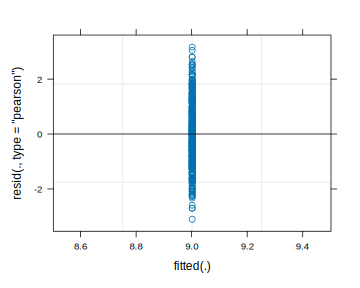
\includegraphics{BIO8940_book_files/figure-latex/mod1_plot-1.pdf}
\caption{(\#fig:mod1\_plot)Fitted values vs residuals for a simple mixed model of unicorn aggression}
\end{figure}

So we can probably do better at modelling the data, which may or may not change our view on whether there is any real variation among unicorns in aggressiveness.

For instance, we can (and should have started with) an initial plot of the phenotypic data against opponent size indicates to have a look at our prediction.

The code below uses the excellent 📦 \texttt{ggplot2} but the same figure can be done using base R code.

\begin{Shaded}
\begin{Highlighting}[]
\FunctionTok{ggplot}\NormalTok{(unicorns, }\FunctionTok{aes}\NormalTok{(}\AttributeTok{x =}\NormalTok{ opp\_size, }\AttributeTok{y =}\NormalTok{ aggression)) }\SpecialCharTok{+}
  \FunctionTok{geom\_jitter}\NormalTok{(}
    \AttributeTok{alpha =} \FloatTok{0.5}\NormalTok{,}
    \AttributeTok{width =} \FloatTok{0.05}
\NormalTok{  ) }\SpecialCharTok{+}
  \FunctionTok{scale\_x\_continuous}\NormalTok{(}\AttributeTok{breaks =} \FunctionTok{c}\NormalTok{(}\SpecialCharTok{{-}}\DecValTok{1}\NormalTok{, }\DecValTok{0}\NormalTok{, }\DecValTok{1}\NormalTok{)) }\SpecialCharTok{+}
  \FunctionTok{labs}\NormalTok{(}
    \AttributeTok{x =} \StringTok{"Opponent size (SD)"}\NormalTok{,}
    \AttributeTok{y =} \StringTok{"Aggression"}
\NormalTok{  ) }\SpecialCharTok{+}
  \FunctionTok{theme\_classic}\NormalTok{()}
\end{Highlighting}
\end{Shaded}

\begin{Shaded}
\begin{Highlighting}[]
\FunctionTok{ggplot}\NormalTok{(unicorns, }\FunctionTok{aes}\NormalTok{(}\AttributeTok{x =}\NormalTok{ opp\_size, }\AttributeTok{y =}\NormalTok{ aggression)) }\SpecialCharTok{+}
  \FunctionTok{geom\_jitter}\NormalTok{(}
    \AttributeTok{alpha =} \FloatTok{0.5}\NormalTok{,}
    \AttributeTok{width =} \FloatTok{0.05}
\NormalTok{  ) }\SpecialCharTok{+}
  \FunctionTok{scale\_x\_continuous}\NormalTok{(}\AttributeTok{breaks =} \FunctionTok{c}\NormalTok{(}\SpecialCharTok{{-}}\DecValTok{1}\NormalTok{, }\DecValTok{0}\NormalTok{, }\DecValTok{1}\NormalTok{)) }\SpecialCharTok{+}
  \FunctionTok{labs}\NormalTok{(}
    \AttributeTok{x =} \StringTok{"Opponent size (SD)"}\NormalTok{,}
    \AttributeTok{y =} \StringTok{"Aggression"}
\NormalTok{  ) }\SpecialCharTok{+}
  \FunctionTok{theme\_classic}\NormalTok{()}
\end{Highlighting}
\end{Shaded}

\begin{figure}

{\centering 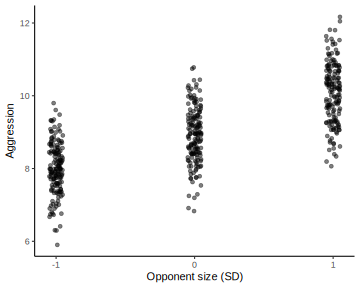
\includegraphics{BIO8940_book_files/figure-latex/rplotaggr-1} 

}

\caption{Unicorn aggressivity as a function of opponent size when fighting for sweets}\label{fig:rplotaggr}
\end{figure}

As predicted, there is a general increase in aggression with opponent size (points are lightly jittered on the x-axis to show the spread of data a little better)

You can see the same thing from a quick look at the population means for aggression at opponent size. Here we do it with the \texttt{kable} function that makes nice tables in \texttt{rmarkdown} documents.

\begin{Shaded}
\begin{Highlighting}[]
\NormalTok{unicorns }\SpecialCharTok{\%\textgreater{}\%}
  \FunctionTok{group\_by}\NormalTok{(opp\_size) }\SpecialCharTok{\%\textgreater{}\%}
  \FunctionTok{summarise}\NormalTok{(}\AttributeTok{mean\_aggr =} \FunctionTok{mean}\NormalTok{(aggression)) }\SpecialCharTok{\%\textgreater{}\%}
\NormalTok{  knitr}\SpecialCharTok{::}\FunctionTok{kable}\NormalTok{(}\AttributeTok{digits =} \DecValTok{2}\NormalTok{)}
\end{Highlighting}
\end{Shaded}

\begin{tabular}{r|r}
\hline
opp\_size & mean\_aggr\\
\hline
-1 & 8.00\\
\hline
0 & 8.91\\
\hline
1 & 10.09\\
\hline
\end{tabular}

So, there does appear to be plasticity of aggression with changing size of the model opponent. But other things may explain variation in aggressiveness too - what about block for instance? Block effects may not be the subject of any biologically interesting hypotheses, but accounting for any differences between blocks could remove noise.

There may also be systematic change in behaviour as an individual experiences more repeat observations (i.e.~exposure to the model). Do they get sensitised or habituated to the model intruder for example?

So let's run a mixed model with the same random effect of individual, but with a fixed effects of opponent size (our predictor of interest) and experimental block.

\begin{Shaded}
\begin{Highlighting}[]
\NormalTok{m\_2 }\OtherTok{\textless{}{-}} \FunctionTok{lmer}\NormalTok{(aggression }\SpecialCharTok{\textasciitilde{}}\NormalTok{ opp\_size  }\SpecialCharTok{+}\NormalTok{ block }\SpecialCharTok{+}\NormalTok{ (}\DecValTok{1} \SpecialCharTok{|}\NormalTok{ ID), }\AttributeTok{data =}\NormalTok{ unicorns)}
\end{Highlighting}
\end{Shaded}

\hypertarget{diagnostic-plots}{%
\subsubsection{Diagnostic plots}\label{diagnostic-plots}}

Run a few diagnostic plots before we look at the answers. In diagnostic plots, we want to check the condition of applications of the linear mixed model which are the same 4 as the linear model plus 2 extra:

\begin{enumerate}
\def\labelenumi{\arabic{enumi}.}
\item
  Linearity of the relation between covariates and the response
\item
  No error on measurement of covariates
\item
  Residual have a Gaussian distribution
\item
  Homoscedasticty (variance of residuals is constant across covariates)
\item
  Random effects have a Gaussian distribution
\item
  Residual variance is constant across all levels of a random effect
\end{enumerate}

This is checked with:

\begin{enumerate}
\def\labelenumi{\arabic{enumi}.}
\tightlist
\item
  done with data exploration graph (i.e.~just plot the data see if it is linear)

  \begin{itemize}
  \tightlist
  \item
    see previous graph
  \end{itemize}
\item
  assumed to be correct if measurement error is lower than 10\% of variance in the variable

  \begin{itemize}
  \tightlist
  \item
    I know this sounds pretty bad
  \end{itemize}
\item
  using quantile-quantile plot or histogram of residuals
\end{enumerate}

\begin{Shaded}
\begin{Highlighting}[]
\FunctionTok{par}\NormalTok{(}\AttributeTok{mfrow =} \FunctionTok{c}\NormalTok{(}\DecValTok{1}\NormalTok{, }\DecValTok{2}\NormalTok{)) }\CommentTok{\# multiple graphs in a window}
\FunctionTok{qqnorm}\NormalTok{(}\FunctionTok{residuals}\NormalTok{(m\_2)) }\CommentTok{\# a q{-}q plot}
\FunctionTok{qqline}\NormalTok{(}\FunctionTok{residuals}\NormalTok{(m\_2))}
\FunctionTok{hist}\NormalTok{(}\FunctionTok{resid}\NormalTok{(m\_2)) }\CommentTok{\# are the residuals roughly Gaussian?}
\end{Highlighting}
\end{Shaded}

\begin{figure}
\centering
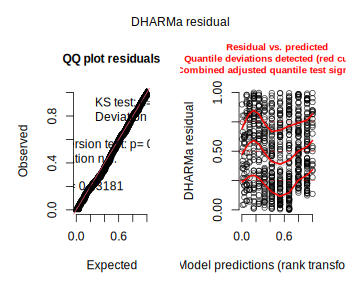
\includegraphics{BIO8940_book_files/figure-latex/unnamed-chunk-14-1.pdf}
\caption{\label{fig:unnamed-chunk-14}Checking residuals have Gaussian distribution}
\end{figure}

\begin{enumerate}
\def\labelenumi{\arabic{enumi}.}
\setcounter{enumi}{3}
\tightlist
\item
  using plot of residuals by fitted values
\end{enumerate}

\begin{Shaded}
\begin{Highlighting}[]
\FunctionTok{plot}\NormalTok{(m\_2)}
\end{Highlighting}
\end{Shaded}

\begin{figure}
\centering
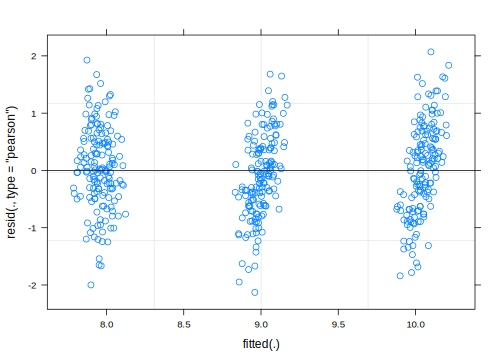
\includegraphics{BIO8940_book_files/figure-latex/unnamed-chunk-15-1.pdf}
\caption{\label{fig:unnamed-chunk-15}Residuals by fitted values for model m\_2 to check homoscedasticity}
\end{figure}

\begin{enumerate}
\def\labelenumi{\arabic{enumi}.}
\setcounter{enumi}{4}
\tightlist
\item
  histogram of the predictions for the random effects (BLUPs)
\end{enumerate}

\begin{Shaded}
\begin{Highlighting}[]
\CommentTok{\# extracting blups}
\NormalTok{r1 }\OtherTok{\textless{}{-}} \FunctionTok{as.data.frame}\NormalTok{(}\FunctionTok{ranef}\NormalTok{(m\_2, }\AttributeTok{condVar =} \ConstantTok{TRUE}\NormalTok{))}

\FunctionTok{par}\NormalTok{(}\AttributeTok{mfrow =} \FunctionTok{c}\NormalTok{(}\DecValTok{1}\NormalTok{, }\DecValTok{2}\NormalTok{))}
\FunctionTok{hist}\NormalTok{(r1}\SpecialCharTok{$}\NormalTok{condval)}
\FunctionTok{qqnorm}\NormalTok{(r1}\SpecialCharTok{$}\NormalTok{condval)}
\FunctionTok{qqline}\NormalTok{(r1}\SpecialCharTok{$}\NormalTok{condval)}
\end{Highlighting}
\end{Shaded}

\begin{figure}
\centering
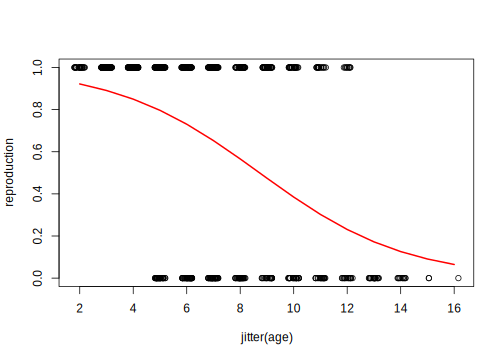
\includegraphics{BIO8940_book_files/figure-latex/unnamed-chunk-16-1.pdf}
\caption{\label{fig:unnamed-chunk-16}Checking random effects are gaussian}
\end{figure}

\begin{enumerate}
\def\labelenumi{\arabic{enumi}.}
\setcounter{enumi}{5}
\tightlist
\item
  plotting the sorted BLUPs with their errors
\end{enumerate}

\begin{Shaded}
\begin{Highlighting}[]
\NormalTok{r1 }\OtherTok{\textless{}{-}}\NormalTok{ r1[}\FunctionTok{order}\NormalTok{(r1}\SpecialCharTok{$}\NormalTok{condval), ] }\CommentTok{\# sorting the BLUPs}
\FunctionTok{ggplot}\NormalTok{(r1, }\FunctionTok{aes}\NormalTok{(}\AttributeTok{y =}\NormalTok{ grp, }\AttributeTok{x =}\NormalTok{ condval)) }\SpecialCharTok{+}
  \FunctionTok{geom\_point}\NormalTok{() }\SpecialCharTok{+}
  \FunctionTok{geom\_pointrange}\NormalTok{(}
    \FunctionTok{aes}\NormalTok{(}\AttributeTok{xmin =}\NormalTok{ condval }\SpecialCharTok{{-}}\NormalTok{ condsd }\SpecialCharTok{*} \FloatTok{1.96}\NormalTok{, }\AttributeTok{xmax =}\NormalTok{ condval }\SpecialCharTok{+}\NormalTok{ condsd }\SpecialCharTok{*} \FloatTok{1.96}\NormalTok{)}
\NormalTok{  ) }\SpecialCharTok{+}
  \FunctionTok{geom\_vline}\NormalTok{(}\FunctionTok{aes}\NormalTok{(}\AttributeTok{xintercept =} \DecValTok{0}\NormalTok{, }\AttributeTok{color =} \StringTok{"red"}\NormalTok{)) }\SpecialCharTok{+}
  \FunctionTok{theme\_classic}\NormalTok{() }\SpecialCharTok{+}
  \FunctionTok{theme}\NormalTok{(}\AttributeTok{legend.position =} \StringTok{"none"}\NormalTok{)}
\end{Highlighting}
\end{Shaded}

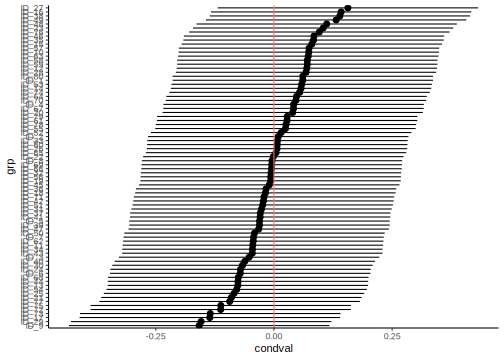
\includegraphics{BIO8940_book_files/figure-latex/mod2_plots-1.pdf}

\hypertarget{inferences}{%
\subsubsection{Inferences}\label{inferences}}

\textbf{Now summarise this model. We will pause here for you to think about and discuss a few things:}
* What can you take from the fixed effect table?
* How do you interpret the intercept now that there are other effects in the model?
* What would happen if we scaled our fixed covariates differently? Why?

\begin{Shaded}
\begin{Highlighting}[]
\FunctionTok{summary}\NormalTok{(m\_2)}
\end{Highlighting}
\end{Shaded}

\begin{verbatim}
## Linear mixed model fit by REML. t-tests use Satterthwaite's method ['lmerModLmerTest']
## Formula: aggression ~ opp_size + block + (1 | ID)
##    Data: unicorns
## 
## REML criterion at convergence: 1129.9
## 
## Scaled residuals: 
##      Min       1Q   Median       3Q      Max 
## -2.79296 -0.64761  0.00155  0.67586  2.71456 
## 
## Random effects:
##  Groups   Name        Variance Std.Dev.
##  ID       (Intercept) 0.02478  0.1574  
##  Residual             0.58166  0.7627  
## Number of obs: 480, groups:  ID, 80
## 
## Fixed effects:
##              Estimate Std. Error        df t value Pr(>|t|)    
## (Intercept)   9.00181    0.03901  79.00000 230.778   <2e-16 ***
## opp_size      1.04562    0.04263 398.00000  24.525   <2e-16 ***
## block        -0.02179    0.06962 398.00000  -0.313    0.754    
## ---
## Signif. codes:  0 '***' 0.001 '**' 0.01 '*' 0.05 '.' 0.1 ' ' 1
## 
## Correlation of Fixed Effects:
##          (Intr) opp_sz
## opp_size 0.000        
## block    0.000  0.000
\end{verbatim}

\begin{rmdcode}
\textbf{Try tweaking the fixed part of your model:}

\begin{itemize}
\tightlist
\item
  What happens if you add more fixed effects? Try it!
\item
  Could focal body size also matter? If so, should you rescale before adding it to the model?
\item
  Should you add interactions (e.g.~block:opp\_size)?
\item
  Should you drop non-significant fixed effects?
\end{itemize}
\end{rmdcode}

\begin{rmdcode}
\textbf{Having changed the fixed part of your model, do the variance estimates change at all?}

\begin{itemize}
\tightlist
\item
  Is among-individual variance always estimated as zero regardless of fixed effects?
\item
  Is among-individual variance significant with some fixed effets structures but not others?
\end{itemize}
\end{rmdcode}

\hypertarget{what-is-the-repeatability}{%
\subsection{What is the repeatability?}\label{what-is-the-repeatability}}

As a reminder, repeatability is the proportion of variance explained by a random effect and it is estimate as the ratio of the variance associated to a random effect by the total variance, or the sum of the residual variance and the different variance compoentn associated with the random effects.
In our first model among-individual variance was zero, so R was zero. If we have a different model of aggression and get a non-zero value of the random effect variance, we can obviously calculate a repeatability estimate (R). So we are all working from the same starting point, let's all stick with a common set of fixed effects from here on:

\begin{Shaded}
\begin{Highlighting}[]
\NormalTok{m\_3 }\OtherTok{\textless{}{-}} \FunctionTok{lmer}\NormalTok{(}
\NormalTok{  aggression }\SpecialCharTok{\textasciitilde{}}\NormalTok{ opp\_size }\SpecialCharTok{+} \FunctionTok{scale}\NormalTok{(body\_size, }\AttributeTok{center =} \ConstantTok{TRUE}\NormalTok{, }\AttributeTok{scale =} \ConstantTok{TRUE}\NormalTok{)}
              \SpecialCharTok{+} \FunctionTok{scale}\NormalTok{(assay\_rep, }\AttributeTok{scale =} \ConstantTok{FALSE}\NormalTok{) }\SpecialCharTok{+}\NormalTok{ block}
              \SpecialCharTok{+}\NormalTok{ (}\DecValTok{1} \SpecialCharTok{|}\NormalTok{ ID),}
  \AttributeTok{data =}\NormalTok{ unicorns)}
\FunctionTok{summary}\NormalTok{(m\_3)}
\end{Highlighting}
\end{Shaded}

\begin{verbatim}
## Linear mixed model fit by REML. t-tests use Satterthwaite's method ['lmerModLmerTest']
## Formula: aggression ~ opp_size + scale(body_size, center = TRUE, scale = TRUE) +      scale(assay_rep, scale = FALSE) + block + (1 | ID)
##    Data: unicorns
## 
## REML criterion at convergence: 1136.5
## 
## Scaled residuals: 
##      Min       1Q   Median       3Q      Max 
## -2.85473 -0.62831  0.02545  0.68998  2.74064 
## 
## Random effects:
##  Groups   Name        Variance Std.Dev.
##  ID       (Intercept) 0.02538  0.1593  
##  Residual             0.58048  0.7619  
## Number of obs: 480, groups:  ID, 80
## 
## Fixed effects:
##                                                Estimate Std. Error        df t value Pr(>|t|)    
## (Intercept)                                     9.00181    0.03907  78.07315 230.395   <2e-16 ***
## opp_size                                        1.05141    0.04281 396.99857  24.562   <2e-16 ***
## scale(body_size, center = TRUE, scale = TRUE)   0.03310    0.03896  84.21144   0.850    0.398    
## scale(assay_rep, scale = FALSE)                -0.05783    0.04281 396.99857  -1.351    0.177    
## block                                          -0.02166    0.06955 397.00209  -0.311    0.756    
## ---
## Signif. codes:  0 '***' 0.001 '**' 0.01 '*' 0.05 '.' 0.1 ' ' 1
## 
## Correlation of Fixed Effects:
##             (Intr) opp_sz sc=Ts=T s(_s=F
## opp_size     0.000                      
## s(_,c=TRs=T  0.000  0.000               
## s(_,s=FALSE  0.000 -0.100  0.000        
## block        0.000  0.000  0.002   0.000
\end{verbatim}

So we'd probably calculate R using the individual and residual variance simply as:

\begin{Shaded}
\begin{Highlighting}[]
\FloatTok{0.02538} \SpecialCharTok{/}\NormalTok{ (}\FloatTok{0.02538} \SpecialCharTok{+} \FloatTok{0.58048}\NormalTok{)}
\end{Highlighting}
\end{Shaded}

\begin{verbatim}
## [1] 0.04189087
\end{verbatim}

\begin{rmdcode}
Do you see where I took the numbers ?
\end{rmdcode}

We can use some more fancy coding to extract the estimates and plugged them in a formula to estimate the repeatbility

\begin{Shaded}
\begin{Highlighting}[]
\NormalTok{v\_id }\OtherTok{\textless{}{-}} \FunctionTok{VarCorr}\NormalTok{(m\_3)}\SpecialCharTok{$}\NormalTok{ID[}\DecValTok{1}\NormalTok{, }\DecValTok{1}\NormalTok{]}
\NormalTok{v\_r }\OtherTok{\textless{}{-}} \FunctionTok{attr}\NormalTok{(}\FunctionTok{VarCorr}\NormalTok{(m\_3), }\StringTok{"sc"}\NormalTok{)}\SpecialCharTok{\^{}}\DecValTok{2}
\NormalTok{r\_man }\OtherTok{\textless{}{-}}\NormalTok{ v\_id }\SpecialCharTok{/}\NormalTok{ (v\_id }\SpecialCharTok{+}\NormalTok{ v\_r)}
\NormalTok{r\_man}
\end{Highlighting}
\end{Shaded}

\begin{verbatim}
## [1] 0.04188879
\end{verbatim}

Which yields an estimate of approximately R=4\%. Strictly speaking we should make clear this a \textbf{conditional repeatability} estimate.

Conditional on what you might ask\ldots{} on the fixed effects in your model. So our best estimate of 4\% refers to the proportion of variance in aggressiveness \emph{not explained by fixed effects} that is explained by individual identity. This isn't much and still won't be significant, but illustrates the point that conditional repeatabilities often have a tendency to go up as people explain more of the residual variance by adding fixed effects. This is fine and proper, but can mislead the unwary reader.
It also means that decisions about which fixed effects to include in your model need to be based on how you want to interpret R not just on, for instance, whether fixed effects are deemed significant.

\hypertarget{a-quick-note-on-uncertainty}{%
\subsection{A quick note on uncertainty}\label{a-quick-note-on-uncertainty}}

Using \texttt{lmer} in the 📦 \texttt{lme4} 📦 there isn't a really simple way to put some measure of uncertainty (SE or CI) on derived parameters like repeatabilities. This is a bit annoying. Such things are more easily done with other mixed model 📦 like \texttt{MCMCglmm} and \texttt{asreml} which are a bit more specialist. If you are using \texttt{lmer} for models you want to publish then you could look into the 📦 \texttt{rptR} \citep{R-rptR}. This acts as a `wrapper' for \texttt{lmer} models and adds some nice functionality including options to boostrap confidence intervals. Regardless, of how you do it, if you want to put a repeatability in one of your papers as a key result - it really should be accompanied by a measure of uncertainty just like any other effect size estimate.

Here I am estimating the repeatability and using bootstrap to estimate a confidence interval and a probability associated with the repeatability with the \texttt{rptR} 📦. For more information about the use of the package and the theory behind it suggest the excellent paper associated with the package \citep{rptR2017}

\begin{Shaded}
\begin{Highlighting}[]
\NormalTok{r\_rpt }\OtherTok{\textless{}{-}} \FunctionTok{rptGaussian}\NormalTok{(}
\NormalTok{  aggression }\SpecialCharTok{\textasciitilde{}}\NormalTok{ opp\_size }\SpecialCharTok{+}\NormalTok{ block }\SpecialCharTok{+}\NormalTok{ (}\DecValTok{1} \SpecialCharTok{|}\NormalTok{ ID),}
  \AttributeTok{grname =} \StringTok{"ID"}\NormalTok{, }\AttributeTok{data =}\NormalTok{ unicorns)}
\end{Highlighting}
\end{Shaded}

\begin{verbatim}
## Bootstrap Progress:
\end{verbatim}

\begin{Shaded}
\begin{Highlighting}[]
\NormalTok{r\_rpt}
\end{Highlighting}
\end{Shaded}

\begin{verbatim}
## 
## 
## Repeatability estimation using the lmm method 
## 
## Repeatability for ID
## R  = 0.041
## SE = 0.031
## CI = [0, 0.108]
## P  = 0.0966 [LRT]
##      NA [Permutation]
\end{verbatim}

\hypertarget{an-easy-way-to-mess-up-your-mixed-models}{%
\subsection{An easy way to mess up your mixed models}\label{an-easy-way-to-mess-up-your-mixed-models}}

We will try some more advanced mixed models in a moment to explore plasticity in aggressiveness a bit more. First let's quickly look for among-individual variance in focal body size. Why not? We have the data handy, everyone says morphological traits are very repeatable and - lets be honest - who wouldn't like to see a small P value after striking out with aggressiveness.

Include a random effect of ID as before and maybe a fixed effect of block, just to see if the beasties were growing a bit between data collection periods.

\begin{Shaded}
\begin{Highlighting}[]
\NormalTok{lmer\_size }\OtherTok{\textless{}{-}} \FunctionTok{lmer}\NormalTok{(body\_size }\SpecialCharTok{\textasciitilde{}}\NormalTok{ block }\SpecialCharTok{+}\NormalTok{ (}\DecValTok{1} \SpecialCharTok{|}\NormalTok{ ID),}
                \AttributeTok{data =}\NormalTok{ unicorns)}
\end{Highlighting}
\end{Shaded}

Summarise and test the random effect.

\begin{Shaded}
\begin{Highlighting}[]
\FunctionTok{summary}\NormalTok{(lmer\_size)}
\end{Highlighting}
\end{Shaded}

\begin{verbatim}
## Linear mixed model fit by REML. t-tests use Satterthwaite's method ['lmerModLmerTest']
## Formula: body_size ~ block + (1 | ID)
##    Data: unicorns
## 
## REML criterion at convergence: 3460.7
## 
## Scaled residuals: 
##      Min       1Q   Median       3Q      Max 
## -1.80452 -0.71319  0.00718  0.70280  1.81747 
## 
## Random effects:
##  Groups   Name        Variance Std.Dev.
##  ID       (Intercept) 936.01   30.594  
##  Residual              34.32    5.858  
## Number of obs: 480, groups:  ID, 80
## 
## Fixed effects:
##             Estimate Std. Error       df t value Pr(>|t|)    
## (Intercept) 252.5031     3.4310  79.0000  73.595   <2e-16 ***
## block        -0.1188     0.5348 399.0000  -0.222    0.824    
## ---
## Signif. codes:  0 '***' 0.001 '**' 0.01 '*' 0.05 '.' 0.1 ' ' 1
## 
## Correlation of Fixed Effects:
##       (Intr)
## block 0.000
\end{verbatim}

\begin{Shaded}
\begin{Highlighting}[]
\FunctionTok{ranova}\NormalTok{(lmer\_size)}
\end{Highlighting}
\end{Shaded}

\begin{verbatim}
## ANOVA-like table for random-effects: Single term deletions
## 
## Model:
## body_size ~ block + (1 | ID)
##          npar  logLik    AIC    LRT Df Pr(>Chisq)    
## <none>      4 -1730.4 3468.7                         
## (1 | ID)    3 -2325.6 4657.1 1190.4  1  < 2.2e-16 ***
## ---
## Signif. codes:  0 '***' 0.001 '**' 0.01 '*' 0.05 '.' 0.1 ' ' 1
\end{verbatim}

\begin{rmdcode}
\textbf{What might you conclude, and why would this be foolish?}
\end{rmdcode}

Hopefully you spotted the problem here. You have fed in a data set with 6 records per individual (with 2 sets of 3 identical values per unicorns), when you know size was only measured twice in reality. This means you'd expect to get a (potentially very) upwardly biased estimate of R and a (potentially very) downwardly biased P value when testing among-individual variance.

\begin{rmdcode}
\textbf{How can we do it properly?}
\end{rmdcode}

We can prune the data to the two actual observations per unicorns by just selecting the first assay in each block.

\begin{Shaded}
\begin{Highlighting}[]
\NormalTok{unicorns2 }\OtherTok{\textless{}{-}}\NormalTok{ unicorns[unicorns}\SpecialCharTok{$}\NormalTok{assay\_rep }\SpecialCharTok{==} \DecValTok{1}\NormalTok{, ]}

\NormalTok{lmer\_size2 }\OtherTok{\textless{}{-}} \FunctionTok{lmer}\NormalTok{(body\_size }\SpecialCharTok{\textasciitilde{}}\NormalTok{   block }\SpecialCharTok{+}\NormalTok{  (}\DecValTok{1} \SpecialCharTok{|}\NormalTok{ ID),}
                \AttributeTok{data =}\NormalTok{ unicorns2)}
\FunctionTok{summary}\NormalTok{(lmer\_size2)}
\end{Highlighting}
\end{Shaded}

\begin{verbatim}
## Linear mixed model fit by REML. t-tests use Satterthwaite's method ['lmerModLmerTest']
## Formula: body_size ~ block + (1 | ID)
##    Data: unicorns2
## 
## REML criterion at convergence: 1373.4
## 
## Scaled residuals: 
##      Min       1Q   Median       3Q      Max 
## -1.54633 -0.56198  0.01319  0.56094  1.42095 
## 
## Random effects:
##  Groups   Name        Variance Std.Dev.
##  ID       (Intercept) 912.84   30.213  
##  Residual              57.78    7.601  
## Number of obs: 160, groups:  ID, 80
## 
## Fixed effects:
##             Estimate Std. Error       df t value Pr(>|t|)    
## (Intercept) 252.5031     3.4310  79.0000  73.595   <2e-16 ***
## block        -0.1188     1.2019  79.0000  -0.099    0.922    
## ---
## Signif. codes:  0 '***' 0.001 '**' 0.01 '*' 0.05 '.' 0.1 ' ' 1
## 
## Correlation of Fixed Effects:
##       (Intr)
## block 0.000
\end{verbatim}

\begin{Shaded}
\begin{Highlighting}[]
\FunctionTok{ranova}\NormalTok{(lmer\_size2)}
\end{Highlighting}
\end{Shaded}

\begin{verbatim}
## ANOVA-like table for random-effects: Single term deletions
## 
## Model:
## body_size ~ block + (1 | ID)
##          npar  logLik    AIC    LRT Df Pr(>Chisq)    
## <none>      4 -686.68 1381.3                         
## (1 | ID)    3 -771.93 1549.9 170.51  1  < 2.2e-16 ***
## ---
## Signif. codes:  0 '***' 0.001 '**' 0.01 '*' 0.05 '.' 0.1 ' ' 1
\end{verbatim}

Summarise and test your random effect and you'll see the qualitative conclusions will actually be very similar using the pruned data set. Of course this won't generallty but be true, so just be careful. Mixed models are intended to help you model repeated measures data with non-independence, but they won't get you out of trouble if you mis-represent the true structure of observations on your dependent variable.

\hypertarget{happy-mixed-modelling}{%
\section{Happy mixed-modelling}\label{happy-mixed-modelling}}

\begin{figure}

{\centering \includegraphics[width=0.2\linewidth]{images/unicorn} 

}

\caption{The superb unicorn}\label{fig:unnamed-chunk-26}
\end{figure}

\hypertarget{introduction-to-glmm}{%
\chapter{\texorpdfstring{Introduction to \texttt{GLMM}}{Introduction to GLMM}}\label{introduction-to-glmm}}

\hypertarget{practical-3}{%
\section{Practical}\label{practical-3}}

Spatial variation in nutrient availability and herbivory is likely to cause pop-ulation differentiation and maintain genetic diversity in plant populations.Here we measure the extent to which mouse-ear cress (Arabidopsis thaliana)exhibits population and genotypic variation in their responses to these im-portant environmental factors. We are particularly interested in whetherthese populations exhibit nutrient mediated compensation, where higher nutrient levels allow genotypes to better tolerate herbivory (Banta et al.,2010). We use GLMMs to estimate the effect of nutrient levels, simulated hebivory, and their interaction on fruit production in Arabidopsis thaliana(fixed effects), and the extent to which populations vary in their responses(random effects, or variance components)

\hypertarget{packages-and-functions}{%
\subsection{Packages and functions}\label{packages-and-functions}}

You need to download the ``extra\_funs.R'' script for some functions used in the Practical

\begin{Shaded}
\begin{Highlighting}[]
\FunctionTok{library}\NormalTok{(lme4)}
\FunctionTok{library}\NormalTok{(tidyverse)}
\FunctionTok{library}\NormalTok{(patchwork)}
\FunctionTok{library}\NormalTok{(lattice)}
\FunctionTok{source}\NormalTok{(}\StringTok{"data/extra\_funs.R"}\NormalTok{)}
\end{Highlighting}
\end{Shaded}

\hypertarget{the-data-set}{%
\subsection{The data set}\label{the-data-set}}

In this data set, the response variable is the number of fruits (i.e.~seedcapsules) per plant. The number of fruits produced by an individual plant(the experimental unit) was hypothesized to be a function of fixed effects,including nutrient levels (low vs.~high), simulated herbivory (none vs.~apicalmeristem damage), region (Sweden, Netherlands, Spain), and interactionsamong these. Fruit number was also a function of random effects including both the population and individual genotype. Because Arabidopsis is highlyselfing, seeds of a single individual served as replicates of that individual.There were also nuisance variables, including the placement of the plantin the greenhouse, and the method used to germinate seeds. These were estimated as fixed effects but interactions were excluded.

\begin{itemize}
\tightlist
\item
  \texttt{X} observation number (we will use this observation number later, when we are accounting for overdispersion)
\item
  \texttt{reg} a factor for region (Netherlands, Spain, Sweden).
\item
  \texttt{popu} a factor with a level for each population.
\item
  \texttt{gen} a factor with a level for each genotype.
\item
  \texttt{rack} a nuisance factor for one of two greenhouse racks.
\item
  \texttt{nutrient} a factor with levels for minimal or additional nutrients.
\item
  \texttt{amd} a factor with levels for no damage or simulated herbivory (apical meristem damage; we will sometimes refer to this as ``clipping'')
\item
  \texttt{status} a nuisance factor for germination method.
\item
  \texttt{total.fruits} the response; an integer count of the number of fruits perplant.
\end{itemize}

\hypertarget{specifying-fixed-and-random-effects}{%
\subsection{Specifying fixed and random Effects}\label{specifying-fixed-and-random-effects}}

Here we need to select a realistic full model, based on the scientific ques-tions and the data actually at hand. We first load the data set and makesure that each variable is appropriately designated as numeric or factor (i.e.categorical variable).

\begin{Shaded}
\begin{Highlighting}[]
\NormalTok{dat\_tf }\OtherTok{\textless{}{-}} \FunctionTok{read.csv}\NormalTok{(}\StringTok{"data/Banta\_TotalFruits.csv"}\NormalTok{)}
\FunctionTok{str}\NormalTok{(dat\_tf)}
\end{Highlighting}
\end{Shaded}

\begin{verbatim}
## 'data.frame':    625 obs. of  9 variables:
##  $ X           : int  1 2 3 4 5 6 7 8 9 10 ...
##  $ reg         : chr  "NL" "NL" "NL" "NL" ...
##  $ popu        : chr  "3.NL" "3.NL" "3.NL" "3.NL" ...
##  $ gen         : int  4 4 4 4 4 4 4 4 4 5 ...
##  $ rack        : int  2 1 1 2 2 2 2 1 2 1 ...
##  $ nutrient    : int  1 1 1 1 8 1 1 1 8 1 ...
##  $ amd         : chr  "clipped" "clipped" "clipped" "clipped" ...
##  $ status      : chr  "Transplant" "Petri.Plate" "Normal" "Normal" ...
##  $ total.fruits: int  0 0 0 0 0 0 0 3 2 0 ...
\end{verbatim}

The \texttt{X}, \texttt{gen}, \texttt{rack} and \texttt{nutrient} variables are coded as integers, but we want them to be factors.
ˆ We use transform(), which operates within the data set, to avoid typing lots of commands like \texttt{dat\_tf\$rack\ \textless{}-\ factor(dat\_tf\$rack)}
ˆ At the same time, we reorder the \texttt{clipping} variable so that \texttt{"unclipped"} is the reference level (we could also have used \texttt{relevel(amd,"unclipped")}).

\begin{Shaded}
\begin{Highlighting}[]
\NormalTok{dat\_tf }\OtherTok{\textless{}{-}} \FunctionTok{mutate}\NormalTok{(}
\NormalTok{  dat\_tf,}
  \AttributeTok{X =} \FunctionTok{factor}\NormalTok{(X),}
  \AttributeTok{gen =} \FunctionTok{factor}\NormalTok{(gen),}
  \AttributeTok{rack =} \FunctionTok{factor}\NormalTok{(rack),}
  \AttributeTok{amd =} \FunctionTok{factor}\NormalTok{(amd, }\AttributeTok{levels =} \FunctionTok{c}\NormalTok{(}\StringTok{"unclipped"}\NormalTok{, }\StringTok{"clipped"}\NormalTok{)),}
  \AttributeTok{nutrient =} \FunctionTok{factor}\NormalTok{(nutrient, }\AttributeTok{label =} \FunctionTok{c}\NormalTok{(}\StringTok{"Low"}\NormalTok{, }\StringTok{"High"}\NormalTok{))}
\NormalTok{)}
\end{Highlighting}
\end{Shaded}

Now we check replication for each genotype (columns) within each population (rows).

\begin{Shaded}
\begin{Highlighting}[]
\NormalTok{(reptab }\OtherTok{\textless{}{-}} \FunctionTok{with}\NormalTok{(dat\_tf, }\FunctionTok{table}\NormalTok{(popu, gen)))}
\end{Highlighting}
\end{Shaded}

\begin{verbatim}
##       gen
## popu    4  5  6 11 12 13 14 15 16 17 18 19 20 21 22 23 24 25 27 28 30 34 35 36
##   1.SP  0  0  0  0  0 39 26 35  0  0  0  0  0  0  0  0  0  0  0  0  0  0  0  0
##   1.SW  0  0  0  0  0  0  0  0  0  0  0  0  0  0  0  0  0 28 20  0  0  0  0  0
##   2.SW  0  0  0  0  0  0  0  0  0  0  0  0  0  0  0  0  0  0  0 18 14  0  0  0
##   3.NL 31 11 13  0  0  0  0  0  0  0  0  0  0  0  0  0  0  0  0  0  0  0  0  0
##   5.NL  0  0  0 35 26  0  0  0  0  0  0  0  0  0  0  0  0  0  0  0  0  0  0  0
##   5.SP  0  0  0  0  0  0  0  0 43 22 12  0  0  0  0  0  0  0  0  0  0  0  0  0
##   6.SP  0  0  0  0  0  0  0  0  0  0  0 13 24 14  0  0  0  0  0  0  0  0  0  0
##   7.SW  0  0  0  0  0  0  0  0  0  0  0  0  0  0  0  0  0  0  0  0  0 45 47 45
##   8.SP  0  0  0  0  0  0  0  0  0  0  0  0  0  0 13 16 35  0  0  0  0  0  0  0
\end{verbatim}

\begin{rmdcode}
\textbf{Exercise}: this mode of inspection is OK for this data set but might fail for much larger data sets or for more levels of nesting. See if you can think of some other numerical or graphical methods for inspecting the structure of data sets.

\begin{enumerate}
\def\labelenumi{\arabic{enumi}.}
\tightlist
\item
  plot(reptab) gives a mosaic plot of the two-way table; examine this, see if you can figure out how to interpret it, and decide whether you think it might be useful
\item
  try the commands colSums(reptab\textgreater0) (and the equivalent for rowSums) and figure out what they are telling you.
\item
  Using this recipe, how would you compute the range of number of genotypes per treatment combination?
\end{enumerate}
\end{rmdcode}

\begin{enumerate}
\def\labelenumi{\arabic{enumi}.}
\tightlist
\item
  Do you find the mosaic plot you obtained ugly and super hard to read? Me too 🤣
\end{enumerate}

\begin{Shaded}
\begin{Highlighting}[]
\FunctionTok{plot}\NormalTok{(reptab)}
\end{Highlighting}
\end{Shaded}

\begin{figure}
\centering
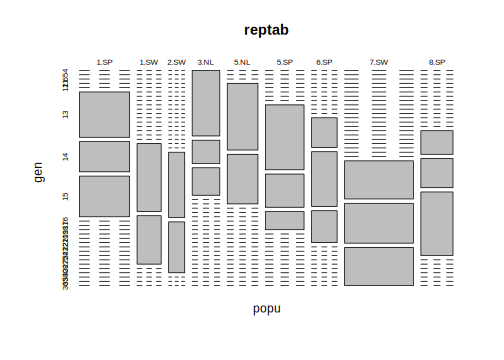
\includegraphics{BIO8940_book_files/figure-latex/unnamed-chunk-32-1.pdf}
\caption{\label{fig:unnamed-chunk-32}A truly useless plot no one can understand}
\end{figure}

\begin{enumerate}
\def\labelenumi{\arabic{enumi}.}
\setcounter{enumi}{1}
\tightlist
\item
  \texttt{colSums()} do the sum of all the rows for each columns of a table. So \texttt{colSums(reptab\textgreater{}0)} gives you for each genotype the number of populations (lines) where you have at least 1 observations.
\end{enumerate}

\begin{Shaded}
\begin{Highlighting}[]
\FunctionTok{colSums}\NormalTok{(reptab }\SpecialCharTok{\textgreater{}} \DecValTok{0}\NormalTok{)}
\end{Highlighting}
\end{Shaded}

\begin{verbatim}
##  4  5  6 11 12 13 14 15 16 17 18 19 20 21 22 23 24 25 27 28 30 34 35 36 
##  1  1  1  1  1  1  1  1  1  1  1  1  1  1  1  1  1  1  1  1  1  1  1  1
\end{verbatim}

\begin{Shaded}
\begin{Highlighting}[]
\FunctionTok{rowSums}\NormalTok{(reptab }\SpecialCharTok{\textgreater{}} \DecValTok{0}\NormalTok{)}
\end{Highlighting}
\end{Shaded}

\begin{verbatim}
## 1.SP 1.SW 2.SW 3.NL 5.NL 5.SP 6.SP 7.SW 8.SP 
##    3    2    2    3    2    3    3    3    3
\end{verbatim}

\begin{enumerate}
\def\labelenumi{\arabic{enumi}.}
\setcounter{enumi}{2}
\tightlist
\item
  You firts need to create a new table of number of observations per treatment and genotypes
\end{enumerate}

\begin{Shaded}
\begin{Highlighting}[]
\NormalTok{reptab2 }\OtherTok{\textless{}{-}} \FunctionTok{with}\NormalTok{(dat\_tf, }\FunctionTok{table}\NormalTok{(}\FunctionTok{paste}\NormalTok{(amd, nutrient, }\AttributeTok{sep =} \StringTok{"\_"}\NormalTok{), gen))}
\FunctionTok{range}\NormalTok{(reptab2)}
\end{Highlighting}
\end{Shaded}

\begin{verbatim}
## [1]  2 13
\end{verbatim}

This reveals that we have only 2--4 populations per region and 2--3 genotypes per population. However, we also have 2--13 replicates per genotype for each treatment combination (four unique treatment combinations: 2 levels of nutrients by 2 levels of simulated herbivory). Thus, even though this was a reasonably large experiment (625 plants), there were a very small number of replicates with which to estimate variance components, and many more potential interactions than our data can support. Therefore, judicious selection of model terms, based on both biology and the data, is warranted. We note that we don't really have enough levels per random effect, nor enough replication per unique treatment combination. Therefore, we decide to omit the fixed effect of ``region'', although we recognize that populations in different regions are widely geographically separated.

However, as in all GLMMs where the scale parameter is treated as fixed and deviations from the fixed scale parameter would be identifiable (i.e.~Poisson and binomial (N \textgreater{} 1), but not binary, models) we may have to deal with overdispersion.

\hypertarget{look-at-overall-patterns-in-data}{%
\subsection{Look at overall patterns in data}\label{look-at-overall-patterns-in-data}}

I usually like to start with a relatively simple overall plot of the data, disregarding the random factors, just to see what's going on. For reasons to be discussed below, we choose to look at the data on the log (or log(1 + x) scale. Let's plot either box-and-whisker plots (useful summaries) or dot plots (more detailed, good for seeing if we missed anything).

\begin{figure}
\centering
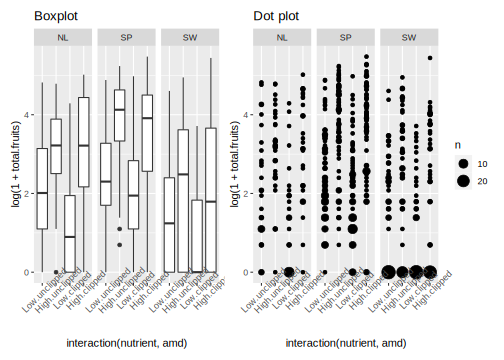
\includegraphics{BIO8940_book_files/figure-latex/unnamed-chunk-35-1.pdf}
\caption{\label{fig:unnamed-chunk-35}Number of fruits (log + 1) as a function of treatments}
\end{figure}

\begin{rmdcode}
\textbf{Exercise} generate these plots and figure out how they work before continuing. Try conditioning/faceting on population rather than region: for facet\_wrap you might want to take out the nrow=1 specification. If you want try reorder the subplots by overall mean fruit set and/or colour the points according to the region they come from.
\end{rmdcode}

\begin{Shaded}
\begin{Highlighting}[]
\NormalTok{p1 }\OtherTok{\textless{}{-}} \FunctionTok{qplot}\NormalTok{(}
    \FunctionTok{interaction}\NormalTok{(nutrient, amd),}
    \FunctionTok{log}\NormalTok{(}\DecValTok{1} \SpecialCharTok{+}\NormalTok{ total.fruits),}
    \AttributeTok{data =}\NormalTok{ dat\_tf, }\AttributeTok{geom =} \StringTok{"boxplot"}\NormalTok{) }\SpecialCharTok{+}
  \FunctionTok{facet\_wrap}\NormalTok{(}\SpecialCharTok{\textasciitilde{}}\NormalTok{reg, }\AttributeTok{nrow =} \DecValTok{1}\NormalTok{) }\SpecialCharTok{+}
  \FunctionTok{theme}\NormalTok{(}\AttributeTok{axis.text.x =} \FunctionTok{element\_text}\NormalTok{(}\AttributeTok{angle =} \DecValTok{45}\NormalTok{)) }\SpecialCharTok{+}
  \FunctionTok{ggtitle}\NormalTok{(}\StringTok{"Boxplot"}\NormalTok{)}
\NormalTok{p2 }\OtherTok{\textless{}{-}} \FunctionTok{qplot}\NormalTok{(}
    \FunctionTok{interaction}\NormalTok{(nutrient, amd),}
    \FunctionTok{log}\NormalTok{(}\DecValTok{1} \SpecialCharTok{+}\NormalTok{ total.fruits),}
    \AttributeTok{data =}\NormalTok{ dat\_tf) }\SpecialCharTok{+}
  \FunctionTok{facet\_wrap}\NormalTok{(}\SpecialCharTok{\textasciitilde{}}\NormalTok{reg, }\AttributeTok{nrow =} \DecValTok{1}\NormalTok{) }\SpecialCharTok{+}
  \FunctionTok{stat\_sum}\NormalTok{() }\SpecialCharTok{+}
  \FunctionTok{theme}\NormalTok{(}\AttributeTok{axis.text.x =} \FunctionTok{element\_text}\NormalTok{(}\AttributeTok{angle =} \DecValTok{45}\NormalTok{)) }\SpecialCharTok{+}
  \FunctionTok{ggtitle}\NormalTok{(}\StringTok{"Dot plot"}\NormalTok{)}
\NormalTok{p1 }\SpecialCharTok{+}\NormalTok{ p2}
\end{Highlighting}
\end{Shaded}

\hypertarget{choose-an-error-distribution}{%
\subsection{Choose an error distribution}\label{choose-an-error-distribution}}

The data are non-normal in principle (i.e., count data, so our first guess would be a Poisson distribution). If we transform total fruits with the canonical link function (log), we hope to see relatively homogeneous variances across categories and groups.

First we define a new factor that represents every combination of genotype and treatment (nutrient × clipping) treatment, and sort it in order of increasing mean fruit set.

\begin{Shaded}
\begin{Highlighting}[]
\NormalTok{dat\_tf }\OtherTok{\textless{}{-}}\NormalTok{ dat\_tf }\SpecialCharTok{\%\textgreater{}\%}
  \FunctionTok{mutate}\NormalTok{(}
    \AttributeTok{gna =} \FunctionTok{reorder}\NormalTok{(}\FunctionTok{interaction}\NormalTok{(gen, nutrient, amd), total.fruits, mean)}
\NormalTok{  )}
\end{Highlighting}
\end{Shaded}

Now time to plot it

\begin{Shaded}
\begin{Highlighting}[]
\FunctionTok{ggplot}\NormalTok{(dat\_tf, }\FunctionTok{aes}\NormalTok{(}\AttributeTok{x =}\NormalTok{ gna, }\AttributeTok{y =} \FunctionTok{log}\NormalTok{(}\DecValTok{1} \SpecialCharTok{+}\NormalTok{ total.fruits))) }\SpecialCharTok{+}
  \FunctionTok{geom\_boxplot}\NormalTok{() }\SpecialCharTok{+}
  \FunctionTok{theme\_bw}\NormalTok{() }\SpecialCharTok{+}
  \FunctionTok{theme}\NormalTok{(}\AttributeTok{axis.text.x =} \FunctionTok{element\_text}\NormalTok{(}\AttributeTok{angle =} \DecValTok{90}\NormalTok{))}
\end{Highlighting}
\end{Shaded}

\begin{figure}
\centering
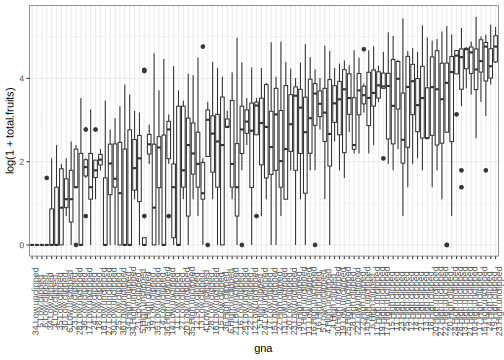
\includegraphics{BIO8940_book_files/figure-latex/unnamed-chunk-39-1.pdf}
\caption{\label{fig:unnamed-chunk-39}Boxplot of total fruits (log + 1) per genotypes and treatments}
\end{figure}

We could also calculate the variance for each genotype × treatment combination and provide a statistical summary of these variances.
This reveals substantial variation among the sample variances on the transformed data. In addition to heterogeneous variances across groups, Figure 1 reveals many zeroes in groups, and some groups with a mean and variance of zero, further suggesting we need a non-normal error distribution, and perhaps something other than a Poisson distribution.

We could calculate λ(mean) for each genotype × treatment combination and provide a statistical summary of each group's λ.

\begin{Shaded}
\begin{Highlighting}[]
\NormalTok{grp\_means }\OtherTok{\textless{}{-}} \FunctionTok{with}\NormalTok{(dat\_tf, }\FunctionTok{tapply}\NormalTok{(total.fruits, }\FunctionTok{list}\NormalTok{(gna), mean))}
\FunctionTok{summary}\NormalTok{(grp\_means)}
\end{Highlighting}
\end{Shaded}

\begin{verbatim}
##    Min. 1st Qu.  Median    Mean 3rd Qu.    Max. 
##    0.00   11.35   23.16   31.86   49.74  122.40
\end{verbatim}

A core property of the Poisson distribution is that the variance is equal to the mean. A simple diagnostic is a plot of the group variances against the group means:

\begin{itemize}
\tightlist
\item
  Poisson-distributed data will result in a linear pattern with slope = 1
\item
  as long as the variance is generally greater than the mean, we call the data overdispersed. Overdispersion comes in various forms:

  \begin{itemize}
  \tightlist
  \item
    a linear mean-variance relationship with Var = φµ (a line through the origin) with φ \textgreater{} 1 is called a quasi-Poisson pattern (this term describes the mean-variance relationship, not any particular proability distribution); we can implement it statistically via quasilikelihood (Venables and Ripley, 2002) or by using a particular parameterization of the negative binomial distribution (``NB1'' inthe terminology of Hardin and Hilbe (2007))
  \item
    a semi-quadratic pattern, Var = µ(1 + αµ) or µ(1 + µ/k), is characteristic of overdispersed data that is driven by underlying heterogeneity among samples, either the negative binomial (gamma-Poisson) or the lognormal-Poisson \citep{elston2001}
  \end{itemize}
\end{itemize}

We've already calculated the group (genotype × treatment) means, we calculate the variances in the same way.

\begin{Shaded}
\begin{Highlighting}[]
\NormalTok{grp\_vars }\OtherTok{\textless{}{-}} \FunctionTok{with}\NormalTok{(}
\NormalTok{  dat\_tf,}
  \FunctionTok{tapply}\NormalTok{(}
\NormalTok{    total.fruits,}
    \FunctionTok{list}\NormalTok{(gna), var}
\NormalTok{  )}
\NormalTok{)}
\end{Highlighting}
\end{Shaded}

We can get approximate estimates of the quasi-Poisson (linear) and negative binomial (linear/quadratic) pattern using lm.

\begin{Shaded}
\begin{Highlighting}[]
\NormalTok{lm1 }\OtherTok{\textless{}{-}} \FunctionTok{lm}\NormalTok{(grp\_vars }\SpecialCharTok{\textasciitilde{}}\NormalTok{ grp\_means }\SpecialCharTok{{-}} \DecValTok{1}\NormalTok{) }\DocumentationTok{\#\# \textasciigrave{}quasi{-}Poisson\textquotesingle{} fit}
\NormalTok{phi\_fit }\OtherTok{\textless{}{-}} \FunctionTok{coef}\NormalTok{(lm1)}
\NormalTok{lm2 }\OtherTok{\textless{}{-}} \FunctionTok{lm}\NormalTok{((grp\_vars }\SpecialCharTok{{-}}\NormalTok{ grp\_means) }\SpecialCharTok{\textasciitilde{}} \FunctionTok{I}\NormalTok{(grp\_means}\SpecialCharTok{\^{}}\DecValTok{2}\NormalTok{) }\SpecialCharTok{{-}} \DecValTok{1}\NormalTok{)}
\NormalTok{k\_fit }\OtherTok{\textless{}{-}} \DecValTok{1} \SpecialCharTok{/} \FunctionTok{coef}\NormalTok{(lm2)}
\end{Highlighting}
\end{Shaded}

Now we can plot them.

\begin{Shaded}
\begin{Highlighting}[]
\FunctionTok{plot}\NormalTok{(grp\_vars }\SpecialCharTok{\textasciitilde{}}\NormalTok{ grp\_means, }\AttributeTok{xlab =} \StringTok{"group means"}\NormalTok{, }\AttributeTok{ylab =} \StringTok{"group variances"}\NormalTok{)}
\FunctionTok{abline}\NormalTok{(}\FunctionTok{c}\NormalTok{(}\DecValTok{0}\NormalTok{, }\DecValTok{1}\NormalTok{), }\AttributeTok{lty =} \DecValTok{2}\NormalTok{)}
\FunctionTok{text}\NormalTok{(}\DecValTok{105}\NormalTok{, }\DecValTok{500}\NormalTok{, }\StringTok{"Poisson"}\NormalTok{)}
\FunctionTok{curve}\NormalTok{(phi\_fit }\SpecialCharTok{*}\NormalTok{ x, }\AttributeTok{col =} \DecValTok{2}\NormalTok{, }\AttributeTok{add =} \ConstantTok{TRUE}\NormalTok{)}
\DocumentationTok{\#\# bquote() is used to substitute numeric values}
\DocumentationTok{\#\# in equations with symbols}
\FunctionTok{text}\NormalTok{(}\DecValTok{110}\NormalTok{, }\DecValTok{3900}\NormalTok{,}
  \FunctionTok{bquote}\NormalTok{(}\FunctionTok{paste}\NormalTok{(}\StringTok{"QP: "}\NormalTok{, sigma}\SpecialCharTok{\^{}}\DecValTok{2} \SpecialCharTok{==}\NormalTok{ .(}\FunctionTok{round}\NormalTok{(phi\_fit, }\DecValTok{1}\NormalTok{)) }\SpecialCharTok{*}\NormalTok{ mu)),}
  \AttributeTok{col =} \DecValTok{2}
\NormalTok{)}
\FunctionTok{curve}\NormalTok{(x }\SpecialCharTok{*}\NormalTok{ (}\DecValTok{1} \SpecialCharTok{+}\NormalTok{ x }\SpecialCharTok{/}\NormalTok{ k\_fit), }\AttributeTok{col =} \DecValTok{4}\NormalTok{, }\AttributeTok{add =} \ConstantTok{TRUE}\NormalTok{)}
\FunctionTok{text}\NormalTok{(}\DecValTok{104}\NormalTok{, }\DecValTok{7200}\NormalTok{, }\FunctionTok{paste}\NormalTok{(}\StringTok{"NB: k="}\NormalTok{, }\FunctionTok{round}\NormalTok{(k\_fit, }\DecValTok{1}\NormalTok{), }\AttributeTok{sep =} \StringTok{""}\NormalTok{), }\AttributeTok{col =} \DecValTok{4}\NormalTok{)}
\NormalTok{l\_fit }\OtherTok{\textless{}{-}} \FunctionTok{loess}\NormalTok{(grp\_vars }\SpecialCharTok{\textasciitilde{}}\NormalTok{ grp\_means)}
\NormalTok{mvec }\OtherTok{\textless{}{-}} \DecValTok{0}\SpecialCharTok{:}\DecValTok{120}
\FunctionTok{lines}\NormalTok{(mvec, }\FunctionTok{predict}\NormalTok{(l\_fit, mvec), }\AttributeTok{col =} \DecValTok{5}\NormalTok{)}
\FunctionTok{text}\NormalTok{(}\DecValTok{100}\NormalTok{, }\DecValTok{2500}\NormalTok{, }\StringTok{"loess"}\NormalTok{, }\AttributeTok{col =} \DecValTok{5}\NormalTok{)}
\end{Highlighting}
\end{Shaded}

\begin{figure}
\centering
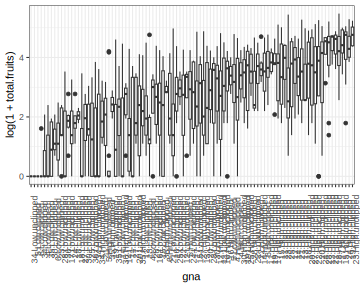
\includegraphics{BIO8940_book_files/figure-latex/unnamed-chunk-43-1.pdf}
\caption{\label{fig:unnamed-chunk-43}Graphical evaluation of distribution to use}
\end{figure}

Same with ggplot

\begin{Shaded}
\begin{Highlighting}[]
\FunctionTok{ggplot}\NormalTok{(}
  \FunctionTok{data.frame}\NormalTok{(grp\_means, grp\_vars),}
  \FunctionTok{aes}\NormalTok{(}\AttributeTok{x =}\NormalTok{ grp\_means, }\AttributeTok{y =}\NormalTok{ grp\_vars)) }\SpecialCharTok{+}
  \FunctionTok{geom\_point}\NormalTok{() }\SpecialCharTok{+}
  \FunctionTok{geom\_smooth}\NormalTok{(}
    \FunctionTok{aes}\NormalTok{(}\AttributeTok{colour =} \StringTok{"Loess"}\NormalTok{), }\AttributeTok{se =} \ConstantTok{FALSE}\NormalTok{) }\SpecialCharTok{+}
  \FunctionTok{geom\_smooth}\NormalTok{(}
    \AttributeTok{method =} \StringTok{"lm"}\NormalTok{, }\AttributeTok{formula =}\NormalTok{ y }\SpecialCharTok{\textasciitilde{}}\NormalTok{ x }\SpecialCharTok{{-}} \DecValTok{1}\NormalTok{, }\AttributeTok{se =} \ConstantTok{FALSE}\NormalTok{,}
    \FunctionTok{aes}\NormalTok{(}\AttributeTok{colour =} \StringTok{"Q\_Pois"}\NormalTok{)) }\SpecialCharTok{+}
  \FunctionTok{stat\_function}\NormalTok{(}
    \AttributeTok{fun =} \ControlFlowTok{function}\NormalTok{(x) x }\SpecialCharTok{*}\NormalTok{ (}\DecValTok{1} \SpecialCharTok{+}\NormalTok{ x }\SpecialCharTok{/}\NormalTok{ k\_fit),}
    \FunctionTok{aes}\NormalTok{(}\AttributeTok{colour =} \StringTok{"Neg\_bin"}\NormalTok{)}
\NormalTok{  ) }\SpecialCharTok{+}
  \FunctionTok{geom\_abline}\NormalTok{(}
    \FunctionTok{aes}\NormalTok{(}\AttributeTok{intercept =} \DecValTok{0}\NormalTok{, }\AttributeTok{slope =} \DecValTok{1}\NormalTok{, }\AttributeTok{colour =} \StringTok{"Poisson"}\NormalTok{)) }\SpecialCharTok{+}
  \FunctionTok{scale\_colour\_manual}\NormalTok{(}
    \AttributeTok{name =} \StringTok{"legend"}\NormalTok{,}
    \AttributeTok{values =} \FunctionTok{c}\NormalTok{(}\StringTok{"blue"}\NormalTok{, }\StringTok{"purple"}\NormalTok{, }\StringTok{"black"}\NormalTok{, }\StringTok{"red"}\NormalTok{)) }\SpecialCharTok{+}
  \FunctionTok{scale\_fill\_manual}\NormalTok{(}
    \AttributeTok{name =} \StringTok{"legend"}\NormalTok{,}
    \AttributeTok{values =} \FunctionTok{c}\NormalTok{(}\StringTok{"blue"}\NormalTok{, }\StringTok{"purple"}\NormalTok{, }\StringTok{"black"}\NormalTok{, }\StringTok{"red"}\NormalTok{)) }\SpecialCharTok{+}
  \FunctionTok{guides}\NormalTok{(}\AttributeTok{fill =} \ConstantTok{FALSE}\NormalTok{)}
\end{Highlighting}
\end{Shaded}

\begin{verbatim}
## `geom_smooth()` using method = 'loess' and formula 'y ~ x'
\end{verbatim}

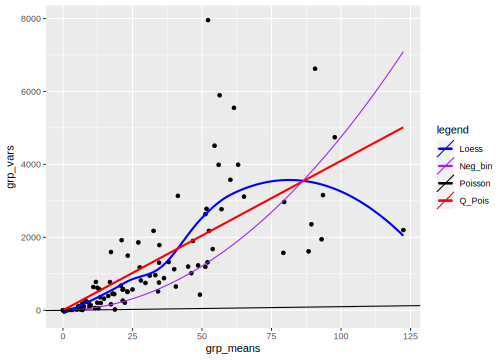
\includegraphics{BIO8940_book_files/figure-latex/unnamed-chunk-44-1.pdf}

These fits are not rigorous statistical tests --- they violate a variety of assumptions of linear regression (e.g.~constant variance, independence), but they are good enough to give us an initial guess about what distributions we should use.

\textbf{Exercise}

\begin{itemize}
\tightlist
\item
  compare a simple quadratic fit to the data (i.e., without the linear part) with the negative binomial and quasipoisson fits
\end{itemize}

\begin{Shaded}
\begin{Highlighting}[]
\NormalTok{lm3 }\OtherTok{\textless{}{-}} \FunctionTok{lm}\NormalTok{(grp\_vars }\SpecialCharTok{\textasciitilde{}} \FunctionTok{I}\NormalTok{(grp\_means)}\SpecialCharTok{\^{}}\DecValTok{2} \SpecialCharTok{{-}} \DecValTok{1}\NormalTok{) }\DocumentationTok{\#\# quadratic fit}
\NormalTok{quad\_fit }\OtherTok{\textless{}{-}} \FunctionTok{coef}\NormalTok{(lm3)}

\FunctionTok{ggplot}\NormalTok{(}
  \FunctionTok{data.frame}\NormalTok{(grp\_means, grp\_vars),}
  \FunctionTok{aes}\NormalTok{(}\AttributeTok{x =}\NormalTok{ grp\_means, }\AttributeTok{y =}\NormalTok{ grp\_vars)) }\SpecialCharTok{+}
  \FunctionTok{geom\_point}\NormalTok{() }\SpecialCharTok{+}
  \FunctionTok{geom\_smooth}\NormalTok{(}
    \AttributeTok{method =} \StringTok{"lm"}\NormalTok{, }\AttributeTok{formula =}\NormalTok{ y }\SpecialCharTok{\textasciitilde{}}\NormalTok{ x }\SpecialCharTok{{-}} \DecValTok{1}\NormalTok{, }\AttributeTok{se =} \ConstantTok{FALSE}\NormalTok{,}
    \FunctionTok{aes}\NormalTok{(}\AttributeTok{colour =} \StringTok{"Q\_Pois"}\NormalTok{)) }\SpecialCharTok{+}
  \FunctionTok{stat\_function}\NormalTok{(}
    \AttributeTok{fun =} \ControlFlowTok{function}\NormalTok{(x) x }\SpecialCharTok{*}\NormalTok{ (}\DecValTok{1} \SpecialCharTok{+}\NormalTok{ x }\SpecialCharTok{/}\NormalTok{ k\_fit),}
    \FunctionTok{aes}\NormalTok{(}\AttributeTok{colour =} \StringTok{"Neg\_bin"}\NormalTok{)}
\NormalTok{  ) }\SpecialCharTok{+}
  \FunctionTok{geom\_smooth}\NormalTok{(}
    \AttributeTok{method =} \StringTok{"lm"}\NormalTok{, }\AttributeTok{formula =}\NormalTok{ y }\SpecialCharTok{\textasciitilde{}} \FunctionTok{I}\NormalTok{(x}\SpecialCharTok{\^{}}\DecValTok{2}\NormalTok{) }\SpecialCharTok{{-}} \DecValTok{1}\NormalTok{, }\AttributeTok{se =} \ConstantTok{FALSE}\NormalTok{,}
    \FunctionTok{aes}\NormalTok{(}\AttributeTok{colour =} \StringTok{"Quad"}\NormalTok{)) }\SpecialCharTok{+}
  \FunctionTok{scale\_colour\_manual}\NormalTok{(}
    \AttributeTok{name =} \StringTok{"legend"}\NormalTok{,}
    \AttributeTok{values =} \FunctionTok{c}\NormalTok{(}\StringTok{"blue"}\NormalTok{, }\StringTok{"purple"}\NormalTok{, }\StringTok{"black"}\NormalTok{)) }\SpecialCharTok{+}
  \FunctionTok{scale\_fill\_manual}\NormalTok{(}
    \AttributeTok{name =} \StringTok{"legend"}\NormalTok{,}
    \AttributeTok{values =} \FunctionTok{c}\NormalTok{(}\StringTok{"blue"}\NormalTok{, }\StringTok{"purple"}\NormalTok{, }\StringTok{"black"}\NormalTok{)) }\SpecialCharTok{+}
  \FunctionTok{guides}\NormalTok{(}\AttributeTok{fill =} \ConstantTok{FALSE}\NormalTok{)}
\end{Highlighting}
\end{Shaded}

\begin{figure}
\centering
\includegraphics{BIO8940_book_files/figure-latex/unnamed-chunk-45-1.pdf}
\caption{\label{fig:unnamed-chunk-45}Graphical evaluation of distribution to use including quadratic effect}
\end{figure}

\hypertarget{plotting-the-response-vs-treatments}{%
\subsubsection{Plotting the response vs treatments}\label{plotting-the-response-vs-treatments}}

Just to avoid surprises

\begin{Shaded}
\begin{Highlighting}[]
\FunctionTok{ggplot}\NormalTok{(dat\_tf, }\FunctionTok{aes}\NormalTok{(}\AttributeTok{x =}\NormalTok{ amd, }\AttributeTok{y =} \FunctionTok{log}\NormalTok{(total.fruits }\SpecialCharTok{+} \DecValTok{1}\NormalTok{), }\AttributeTok{colour =}\NormalTok{ nutrient)) }\SpecialCharTok{+}
  \FunctionTok{geom\_point}\NormalTok{() }\SpecialCharTok{+}
  \DocumentationTok{\#\# need to use as.numeric(amd) to get lines}
  \FunctionTok{stat\_summary}\NormalTok{(}\FunctionTok{aes}\NormalTok{(}\AttributeTok{x =} \FunctionTok{as.numeric}\NormalTok{(amd)), }\AttributeTok{fun =}\NormalTok{ mean, }\AttributeTok{geom =} \StringTok{"line"}\NormalTok{) }\SpecialCharTok{+}
  \FunctionTok{theme\_bw}\NormalTok{() }\SpecialCharTok{+}
  \FunctionTok{theme}\NormalTok{(}\AttributeTok{panel.spacing =} \FunctionTok{unit}\NormalTok{(}\DecValTok{0}\NormalTok{, }\StringTok{"lines"}\NormalTok{)) }\SpecialCharTok{+}
  \FunctionTok{facet\_wrap}\NormalTok{(}\SpecialCharTok{\textasciitilde{}}\NormalTok{popu)}
\end{Highlighting}
\end{Shaded}

\begin{figure}
\centering
\includegraphics{BIO8940_book_files/figure-latex/unnamed-chunk-46-1.pdf}
\caption{\label{fig:unnamed-chunk-46}Fruit production by treatments by population}
\end{figure}

\begin{Shaded}
\begin{Highlighting}[]
\FunctionTok{ggplot}\NormalTok{(dat\_tf, }\FunctionTok{aes}\NormalTok{(}\AttributeTok{x =}\NormalTok{ amd, }\AttributeTok{y =} \FunctionTok{log}\NormalTok{(total.fruits }\SpecialCharTok{+} \DecValTok{1}\NormalTok{), }\AttributeTok{colour =}\NormalTok{ gen)) }\SpecialCharTok{+}
  \FunctionTok{geom\_point}\NormalTok{() }\SpecialCharTok{+}
  \FunctionTok{stat\_summary}\NormalTok{(}\FunctionTok{aes}\NormalTok{(}\AttributeTok{x =} \FunctionTok{as.numeric}\NormalTok{(amd)), }\AttributeTok{fun =}\NormalTok{ mean, }\AttributeTok{geom =} \StringTok{"line"}\NormalTok{) }\SpecialCharTok{+}
  \FunctionTok{theme\_bw}\NormalTok{() }\SpecialCharTok{+}
  \DocumentationTok{\#\# label\_both adds variable name (\textquotesingle{}nutrient\textquotesingle{}) to facet labels}
  \FunctionTok{facet\_grid}\NormalTok{(. }\SpecialCharTok{\textasciitilde{}}\NormalTok{ nutrient, }\AttributeTok{labeller =}\NormalTok{ label\_both)}
\end{Highlighting}
\end{Shaded}

\begin{figure}
\centering
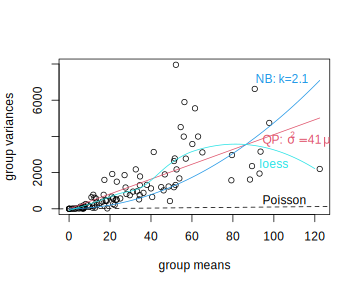
\includegraphics{BIO8940_book_files/figure-latex/unnamed-chunk-47-1.pdf}
\caption{\label{fig:unnamed-chunk-47}Fruit production by genotype by treatments}
\end{figure}

\hypertarget{fitting-group-wise-glm}{%
\subsection{Fitting group-wise GLM}\label{fitting-group-wise-glm}}

Another general starting approach is to fit GLMs to each group of data separately, equivalent to treating the grouping variables as fixed effects.
This should result in reasonable variation among treatment effects. We first fit the models, and then examine the coefficients.

\begin{Shaded}
\begin{Highlighting}[]
\NormalTok{glm\_lis }\OtherTok{\textless{}{-}} \FunctionTok{lmList}\NormalTok{(}
\NormalTok{  total.fruits }\SpecialCharTok{\textasciitilde{}}\NormalTok{ nutrient }\SpecialCharTok{*}\NormalTok{ amd }\SpecialCharTok{|}\NormalTok{ gen,}
  \AttributeTok{data =}\NormalTok{ dat\_tf,}
  \AttributeTok{family =} \StringTok{"poisson"}\NormalTok{)}
\FunctionTok{plot.lmList}\NormalTok{(glm\_lis)}
\end{Highlighting}
\end{Shaded}

\begin{verbatim}
## Using grp as id variables
\end{verbatim}

\begin{figure}
\centering
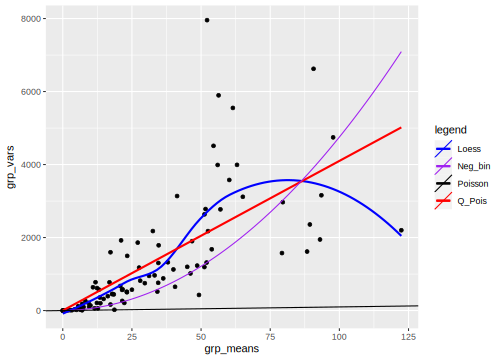
\includegraphics{BIO8940_book_files/figure-latex/unnamed-chunk-48-1.pdf}
\caption{\label{fig:unnamed-chunk-48}Model coefficients for GLM fits on each genotype}
\end{figure}

Three genotypes (5, 6, 34) have extreme coefficients (Fig. 5). A mixed model assumes that the underlying random effects are normally distributed, although we shouldn't take these outliers too seriously at this point --- we are not actually plotting the random effects, or even estimates of random effects (which are not themselves guaranteed to be normally distributed), but rather separate estimates for each group.
Create a plotting function for Q-Q plots of these coefficients to visualize the departure from normality.

\begin{Shaded}
\begin{Highlighting}[]
\FunctionTok{qqmath.lmList}\NormalTok{(glm\_lis)}
\end{Highlighting}
\end{Shaded}

\begin{verbatim}
## Using  as id variables
\end{verbatim}

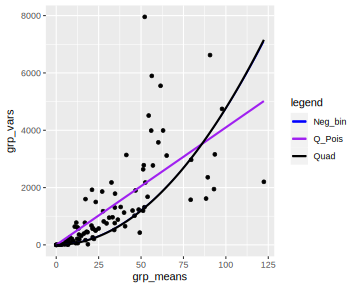
\includegraphics{BIO8940_book_files/figure-latex/unnamed-chunk-49-1.pdf}
We see that these extreme coefficients fall far outside a normal error distribution. We shouldn't take these outliers too seriously at this point --- we are not actually plotting the random effects, or even estimates of random effects, but rather separate estimates for each group.
Especially if these groups have relatively small sample sizes, the estimates may eventually be ``shrunk'' closer to the mean when we do the mixed model.
We should nonetheless take care to see if the coefficients for these genotypes from the GLMM are still outliers, and take the same precautions as we usually do for outliers. For example, we can look back at the original data to see if there is something weird about the way those genotypes were collected, or try re-running the analysis without those genotypes to see if the results are robust.

\hypertarget{fitting-and-evaluating-glmms}{%
\subsection{Fitting and evaluating GLMMs}\label{fitting-and-evaluating-glmms}}

Now we (try to) build and fit a full model, using \texttt{glmer} in the \texttt{emo::ji("pacakage")} \texttt{lme4}. This model has random effects for all genotype and population × treatment random effects, and for the nuisance variables for the rack and germination method (status). (Given the mean-variance relationship we saw it's pretty clear that we are going to have to proceed eventually to a model with overdispersion, but we fit the Poisson model first for illustration.)

\begin{Shaded}
\begin{Highlighting}[]
\NormalTok{mp1 }\OtherTok{\textless{}{-}} \FunctionTok{glmer}\NormalTok{(total.fruits }\SpecialCharTok{\textasciitilde{}}\NormalTok{ nutrient }\SpecialCharTok{*}\NormalTok{ amd }\SpecialCharTok{+}
\NormalTok{  rack }\SpecialCharTok{+}\NormalTok{ status }\SpecialCharTok{+}
\NormalTok{  (amd }\SpecialCharTok{*}\NormalTok{ nutrient }\SpecialCharTok{|}\NormalTok{ popu) }\SpecialCharTok{+}
\NormalTok{  (amd }\SpecialCharTok{*}\NormalTok{ nutrient }\SpecialCharTok{|}\NormalTok{ gen),}
\AttributeTok{data =}\NormalTok{ dat\_tf, }\AttributeTok{family =} \StringTok{"poisson"}
\NormalTok{)}
\end{Highlighting}
\end{Shaded}

\begin{verbatim}
## Warning in checkConv(attr(opt, "derivs"), opt$par, ctrl = control$checkConv, : Model failed to converge with max|grad| = 0.00550538 (tol = 0.002, component 1)
\end{verbatim}

\begin{Shaded}
\begin{Highlighting}[]
\FunctionTok{overdisp\_fun}\NormalTok{(mp1)}
\end{Highlighting}
\end{Shaded}

\begin{verbatim}
##       chisq       ratio           p 
## 13909.46583    23.25998     0.00000
\end{verbatim}

We can ignore the model convergence for the moment. This shows that the data are (extremely) over-dispersed, given the model.

Now we add the observation-level random effect to the model to account for overdispersion \citep{elston2001}.

\begin{Shaded}
\begin{Highlighting}[]
\NormalTok{mp2 }\OtherTok{\textless{}{-}} \FunctionTok{update}\NormalTok{(mp1, . }\SpecialCharTok{\textasciitilde{}}\NormalTok{ . }\SpecialCharTok{+}\NormalTok{ (}\DecValTok{1} \SpecialCharTok{|}\NormalTok{ X))}
\end{Highlighting}
\end{Shaded}

\begin{verbatim}
## Warning in (function (fn, par, lower = rep.int(-Inf, n), upper = rep.int(Inf, : failure to converge in 10000 evaluations
\end{verbatim}

\begin{verbatim}
## Warning in optwrap(optimizer, devfun, start, rho$lower, control = control, : convergence code 4 from Nelder_Mead: failure to converge in 10000 evaluations
\end{verbatim}

\begin{verbatim}
## boundary (singular) fit: see ?isSingular
\end{verbatim}

The model takes much longer to fit (and gives warnings).
We look just at the variance components. In particular, if we look at the correlation matrix among the genotype random effects, we see a perfect
correlation.

\begin{Shaded}
\begin{Highlighting}[]
\FunctionTok{attr}\NormalTok{(}\FunctionTok{VarCorr}\NormalTok{(mp2)}\SpecialCharTok{$}\NormalTok{gen, }\StringTok{"correlation"}\NormalTok{)}
\end{Highlighting}
\end{Shaded}

\begin{verbatim}
##                         (Intercept) amdclipped nutrientHigh amdclipped:nutrientHigh
## (Intercept)               1.0000000 -1.0000000   -0.9856190               0.8102082
## amdclipped               -1.0000000  1.0000000    0.9856458              -0.8103030
## nutrientHigh             -0.9856190  0.9856458    1.0000000              -0.8975369
## amdclipped:nutrientHigh   0.8102082 -0.8103030   -0.8975369               1.0000000
\end{verbatim}

We'll try getting rid of the correlations between clipping (\texttt{amd}) and nutrients, using \texttt{amd+nutrient} instead of \texttt{amd*nutrient} in the random effects specification (here it seems easier to re-do the model rather than using update to add and subtract terms).

\begin{Shaded}
\begin{Highlighting}[]
\NormalTok{mp3 }\OtherTok{\textless{}{-}} \FunctionTok{glmer}\NormalTok{(total.fruits }\SpecialCharTok{\textasciitilde{}}\NormalTok{ nutrient }\SpecialCharTok{*}\NormalTok{ amd }\SpecialCharTok{+}
\NormalTok{  rack }\SpecialCharTok{+}\NormalTok{ status }\SpecialCharTok{+}
\NormalTok{  (amd }\SpecialCharTok{+}\NormalTok{ nutrient }\SpecialCharTok{|}\NormalTok{ popu) }\SpecialCharTok{+}
\NormalTok{  (amd }\SpecialCharTok{+}\NormalTok{ nutrient }\SpecialCharTok{|}\NormalTok{ gen) }\SpecialCharTok{+}\NormalTok{ (}\DecValTok{1} \SpecialCharTok{|}\NormalTok{ X),}
\AttributeTok{data =}\NormalTok{ dat\_tf, }\AttributeTok{family =} \StringTok{"poisson"}
\NormalTok{)}
\end{Highlighting}
\end{Shaded}

\begin{verbatim}
## Warning in checkConv(attr(opt, "derivs"), opt$par, ctrl = control$checkConv, : Model failed to converge with max|grad| = 0.216994 (tol = 0.002, component 1)
\end{verbatim}

\begin{Shaded}
\begin{Highlighting}[]
\FunctionTok{attr}\NormalTok{(}\FunctionTok{VarCorr}\NormalTok{(mp3)}\SpecialCharTok{$}\NormalTok{gen, }\StringTok{"correlation"}\NormalTok{)}
\end{Highlighting}
\end{Shaded}

\begin{verbatim}
##              (Intercept) amdclipped nutrientHigh
## (Intercept)    1.0000000 -0.9998765   -0.9970119
## amdclipped    -0.9998765  1.0000000    0.9969756
## nutrientHigh  -0.9970119  0.9969756    1.0000000
\end{verbatim}

\begin{Shaded}
\begin{Highlighting}[]
\FunctionTok{attr}\NormalTok{(}\FunctionTok{VarCorr}\NormalTok{(mp3)}\SpecialCharTok{$}\NormalTok{popu, }\StringTok{"correlation"}\NormalTok{)}
\end{Highlighting}
\end{Shaded}

\begin{verbatim}
##              (Intercept) amdclipped nutrientHigh
## (Intercept)    1.0000000  0.9958238    0.9947419
## amdclipped     0.9958238  1.0000000    0.9886630
## nutrientHigh   0.9947419  0.9886630    1.0000000
\end{verbatim}

Unfortunately, we still have perfect correlations among the random effects terms. For some models (e.g.~random-slope models), it is possible to fit random effects models in such a way that the correlation between the different parameters (intercept and slope in the case of random-slope models) is constrained to be zero, by fitting a model like \texttt{(1\textbar{}f)+(0+x\textbar{}f)}; unfortunately, because of the way lme4 is set up, this is considerably more difficult with categorical predictors (factors).

We have to reduce the model further in some way in order not to overfit (i.e., in order to not have perfect ±1 correlations among random effects). It looks like we can't allow both nutrients and clipping in the random effect model at either the population or the genotype level. However, it's hard to know whether we should proceed with amd or nutrient, both, or neither in the model.

A convenient way to proceed if we are going to try fitting several different combinations of random effects is to fit the model with all the fixed effects but only observation-level random effects, and then to use update to add various components to it.

\begin{Shaded}
\begin{Highlighting}[]
\NormalTok{mp\_obs }\OtherTok{\textless{}{-}} \FunctionTok{glmer}\NormalTok{(total.fruits }\SpecialCharTok{\textasciitilde{}}\NormalTok{ nutrient }\SpecialCharTok{*}\NormalTok{ amd }\SpecialCharTok{+}
\NormalTok{  rack }\SpecialCharTok{+}\NormalTok{ status }\SpecialCharTok{+}
\NormalTok{  (}\DecValTok{1} \SpecialCharTok{|}\NormalTok{ X),}
\AttributeTok{data =}\NormalTok{ dat\_tf, }\AttributeTok{family =} \StringTok{"poisson"}
\NormalTok{)}
\end{Highlighting}
\end{Shaded}

Now, for example, \texttt{update(mp\_obs,.\textasciitilde{}.+(1\textbar{}gen)+(amd\textbar{}popu))} fits the model with intercept random effects at the genotype level and variation in clipping effects across populations.

\begin{rmdcode}
\textbf{Exercise} using update, fit the models with

\begin{enumerate}
\def\labelenumi{\arabic{enumi}.}
\tightlist
\item
  clipping variation at both genotype and population levels;
\item
  nutrient variation at both genotype and populations; convince yourself that trying to fit variation in either clipping or nutrients leads to overfitting (perfect correlations).
\item
  Fit the model with only intercept variation at the population and genotype levels, saving it as mp4; show that there is non-zero variance estimated
\end{enumerate}
\end{rmdcode}

\begin{enumerate}
\def\labelenumi{\arabic{enumi}.}
\tightlist
\item
\end{enumerate}

\begin{Shaded}
\begin{Highlighting}[]
\NormalTok{mpcli }\OtherTok{\textless{}{-}} \FunctionTok{update}\NormalTok{(mp\_obs, . }\SpecialCharTok{\textasciitilde{}}\NormalTok{ . }\SpecialCharTok{+}\NormalTok{ (amd }\SpecialCharTok{|}\NormalTok{ gen) }\SpecialCharTok{+}\NormalTok{ (amd }\SpecialCharTok{|}\NormalTok{ popu))}
\end{Highlighting}
\end{Shaded}

\begin{verbatim}
## Warning in checkConv(attr(opt, "derivs"), opt$par, ctrl = control$checkConv, : Model failed to converge with max|grad| = 0.115116 (tol = 0.002, component 1)
\end{verbatim}

\begin{Shaded}
\begin{Highlighting}[]
\FunctionTok{VarCorr}\NormalTok{(mpcli)}
\end{Highlighting}
\end{Shaded}

\begin{verbatim}
##  Groups Name        Std.Dev. Corr  
##  X      (Intercept) 1.429806       
##  gen    (Intercept) 0.296991       
##         amdclipped  0.039336 -0.869
##  popu   (Intercept) 0.752718       
##         amdclipped  0.126028 0.995
\end{verbatim}

\begin{enumerate}
\def\labelenumi{\arabic{enumi}.}
\setcounter{enumi}{1}
\tightlist
\item
\end{enumerate}

\begin{Shaded}
\begin{Highlighting}[]
\NormalTok{mpnut }\OtherTok{\textless{}{-}} \FunctionTok{update}\NormalTok{(mp\_obs, . }\SpecialCharTok{\textasciitilde{}}\NormalTok{ . }\SpecialCharTok{+}\NormalTok{ (nutrient }\SpecialCharTok{|}\NormalTok{ gen) }\SpecialCharTok{+}\NormalTok{ (nutrient }\SpecialCharTok{|}\NormalTok{ popu))}
\end{Highlighting}
\end{Shaded}

\begin{verbatim}
## Warning in checkConv(attr(opt, "derivs"), opt$par, ctrl = control$checkConv, : Model failed to converge with max|grad| = 0.0204136 (tol = 0.002, component 1)
\end{verbatim}

\begin{Shaded}
\begin{Highlighting}[]
\FunctionTok{VarCorr}\NormalTok{(mpnut)}
\end{Highlighting}
\end{Shaded}

\begin{verbatim}
##  Groups Name         Std.Dev. Corr  
##  X      (Intercept)  1.41953        
##  gen    (Intercept)  0.47799        
##         nutrientHigh 0.32458  -1.000
##  popu   (Intercept)  0.74706        
##         nutrientHigh 0.12042  1.000
\end{verbatim}

\begin{enumerate}
\def\labelenumi{\arabic{enumi}.}
\setcounter{enumi}{2}
\tightlist
\item
\end{enumerate}

\begin{Shaded}
\begin{Highlighting}[]
\NormalTok{mp4 }\OtherTok{\textless{}{-}} \FunctionTok{update}\NormalTok{(mp\_obs, . }\SpecialCharTok{\textasciitilde{}}\NormalTok{ . }\SpecialCharTok{+}\NormalTok{ (}\DecValTok{1} \SpecialCharTok{|}\NormalTok{ gen) }\SpecialCharTok{+}\NormalTok{ (}\DecValTok{1} \SpecialCharTok{|}\NormalTok{ popu))}
\end{Highlighting}
\end{Shaded}

\begin{verbatim}
## Warning in checkConv(attr(opt, "derivs"), opt$par, ctrl = control$checkConv, : Model failed to converge with max|grad| = 0.00263265 (tol = 0.002, component 1)
\end{verbatim}

\begin{Shaded}
\begin{Highlighting}[]
\FunctionTok{VarCorr}\NormalTok{(mp4)}
\end{Highlighting}
\end{Shaded}

\begin{verbatim}
##  Groups Name        Std.Dev.
##  X      (Intercept) 1.43113 
##  gen    (Intercept) 0.28577 
##  popu   (Intercept) 0.80616
\end{verbatim}

In other words, while it's biologically plausible that there is some variation in the nutrient or clipping effect at the genotype or population levels, with this modeling approach we really don't have enough data to speak confidently about these effects.
Let's check that mp4 no longer incorporates overdispersion (the observationlevel random effect should have taken care of it):

\begin{Shaded}
\begin{Highlighting}[]
\FunctionTok{overdisp\_fun}\NormalTok{(mp4)}
\end{Highlighting}
\end{Shaded}

\begin{verbatim}
##       chisq       ratio           p 
## 177.5567880   0.2887102   1.0000000
\end{verbatim}

\hypertarget{inference}{%
\subsection{Inference}\label{inference}}

\hypertarget{random-effects}{%
\subsubsection{Random effects}\label{random-effects}}

\texttt{glmer} (\texttt{lmer}) does not return information about the standard errors or confidence intervals of the variance components.

\begin{Shaded}
\begin{Highlighting}[]
\FunctionTok{VarCorr}\NormalTok{(mp4)}
\end{Highlighting}
\end{Shaded}

\begin{verbatim}
##  Groups Name        Std.Dev.
##  X      (Intercept) 1.43113 
##  gen    (Intercept) 0.28577 
##  popu   (Intercept) 0.80616
\end{verbatim}

\hypertarget{testing-for-random-effects-1}{%
\paragraph{Testing for random Effects}\label{testing-for-random-effects-1}}

If we want to test the significance of the random effects we can fit reduced models and run likelihood ratio tests via anova, keeping in mind that in this case (testing a null hypothesis of zero variance, where the parameter is on the boundary of its feasible region) the reported p value is approximately twice what it should be.

\begin{Shaded}
\begin{Highlighting}[]
\NormalTok{mp4v1 }\OtherTok{\textless{}{-}} \FunctionTok{update}\NormalTok{(mp\_obs, . }\SpecialCharTok{\textasciitilde{}}\NormalTok{ . }\SpecialCharTok{+}\NormalTok{ (}\DecValTok{1} \SpecialCharTok{|}\NormalTok{ popu)) }\DocumentationTok{\#\# popu only (drop gen)}
\NormalTok{mp4v2 }\OtherTok{\textless{}{-}} \FunctionTok{update}\NormalTok{(mp\_obs, . }\SpecialCharTok{\textasciitilde{}}\NormalTok{ . }\SpecialCharTok{+}\NormalTok{ (}\DecValTok{1} \SpecialCharTok{|}\NormalTok{ gen)) }\DocumentationTok{\#\# gen only (drop popu)}
\end{Highlighting}
\end{Shaded}

\begin{verbatim}
## Warning in checkConv(attr(opt, "derivs"), opt$par, ctrl = control$checkConv, : Model failed to converge with max|grad| = 0.105093 (tol = 0.002, component 1)
\end{verbatim}

\begin{verbatim}
## Warning in checkConv(attr(opt, "derivs"), opt$par, ctrl = control$checkConv, : Model is nearly unidentifiable: very large eigenvalue
##  - Rescale variables?
\end{verbatim}

\begin{Shaded}
\begin{Highlighting}[]
\FunctionTok{anova}\NormalTok{(mp4, mp4v1)}
\end{Highlighting}
\end{Shaded}

\begin{verbatim}
## Data: dat_tf
## Models:
## mp4v1: total.fruits ~ nutrient + amd + rack + status + (1 | X) + (1 | 
## mp4v1:     popu) + nutrient:amd
## mp4: total.fruits ~ nutrient + amd + rack + status + (1 | X) + (1 | 
## mp4:     gen) + (1 | popu) + nutrient:amd
##       npar    AIC    BIC  logLik deviance  Chisq Df Pr(>Chisq)  
## mp4v1    9 5017.4 5057.4 -2499.7   4999.4                       
## mp4     10 5015.4 5059.8 -2497.7   4995.4 4.0638  1    0.04381 *
## ---
## Signif. codes:  0 '***' 0.001 '**' 0.01 '*' 0.05 '.' 0.1 ' ' 1
\end{verbatim}

\begin{Shaded}
\begin{Highlighting}[]
\FunctionTok{anova}\NormalTok{(mp4, mp4v2)}
\end{Highlighting}
\end{Shaded}

\begin{verbatim}
## Data: dat_tf
## Models:
## mp4v2: total.fruits ~ nutrient + amd + rack + status + (1 | X) + (1 | 
## mp4v2:     gen) + nutrient:amd
## mp4: total.fruits ~ nutrient + amd + rack + status + (1 | X) + (1 | 
## mp4:     gen) + (1 | popu) + nutrient:amd
##       npar    AIC    BIC  logLik deviance  Chisq Df Pr(>Chisq)    
## mp4v2    9 5031.6 5071.5 -2506.8   5013.6                         
## mp4     10 5015.4 5059.8 -2497.7   4995.4 18.212  1  1.976e-05 ***
## ---
## Signif. codes:  0 '***' 0.001 '**' 0.01 '*' 0.05 '.' 0.1 ' ' 1
\end{verbatim}

For various forms of linear mixed models, the RLRsim package can do efficient simulation-based hypothesis testing of variance components --- un- fortunately, that doesn't include GLMMs.
If we are sufficiently patient we can do hypothesis testing via brute-force parametric bootstrapping where we repeatedly simulate data from the reduced (null) model, fit both the re- duced and full models to the simulated data, and compute the distribution of the deviance (change in -2 log likelihood).
The code below took about half an hour on a reasonably modern desktop computer.

\begin{Shaded}
\begin{Highlighting}[]
\NormalTok{simdev }\OtherTok{\textless{}{-}} \ControlFlowTok{function}\NormalTok{() \{}
\NormalTok{  newdat }\OtherTok{\textless{}{-}} \FunctionTok{simulate}\NormalTok{(mp4v1)}
\NormalTok{  reduced }\OtherTok{\textless{}{-}}\NormalTok{ lme4}\SpecialCharTok{::}\FunctionTok{refit}\NormalTok{(mp4v1, newdat)}
\NormalTok{  full }\OtherTok{\textless{}{-}}\NormalTok{ lme4}\SpecialCharTok{::}\FunctionTok{refit}\NormalTok{(mp4, newdat)}
  \DecValTok{2} \SpecialCharTok{*}\NormalTok{ (}\FunctionTok{c}\NormalTok{(}\FunctionTok{logLik}\NormalTok{(full) }\SpecialCharTok{{-}} \FunctionTok{logLik}\NormalTok{(reduced)))}
\NormalTok{\}}

\FunctionTok{set.seed}\NormalTok{(}\DecValTok{101}\NormalTok{)}
\NormalTok{nulldist0 }\OtherTok{\textless{}{-}} \FunctionTok{replicate}\NormalTok{(}\DecValTok{2}\NormalTok{, }\FunctionTok{simdev}\NormalTok{())}
\DocumentationTok{\#\# zero spurious (small) negative values}
\NormalTok{nulldist[nulldist }\SpecialCharTok{\textless{}} \DecValTok{0} \SpecialCharTok{\&} \FunctionTok{abs}\NormalTok{(nulldist) }\SpecialCharTok{\textless{}} \FloatTok{1e{-}5}\NormalTok{] }\OtherTok{\textless{}{-}} \DecValTok{0}
\NormalTok{obsdev }\OtherTok{\textless{}{-}} \DecValTok{2} \SpecialCharTok{*} \FunctionTok{c}\NormalTok{(}\FunctionTok{logLik}\NormalTok{(mp4) }\SpecialCharTok{{-}} \FunctionTok{logLik}\NormalTok{(mp4v1))}
\end{Highlighting}
\end{Shaded}

\begin{Shaded}
\begin{Highlighting}[]
\FunctionTok{mean}\NormalTok{(}\FunctionTok{c}\NormalTok{(nulldist, obsdev) }\SpecialCharTok{\textgreater{}=}\NormalTok{ obsdev)}
\end{Highlighting}
\end{Shaded}

\begin{verbatim}
## [1] 0.01492537
\end{verbatim}

The true p-value is actually closer to 0.05 than 0.02. In other words, here the deviations from the original statistical model from that for which the original ``p value is inflated by 2'' rule of thumb was derived --- fitting a GLMM instead of a LMM, and using a moderate-sized rather than an arbitrarily large (asymptotic) data set --- have made the likelihood ratio test liberal (increased type I error) rather than conservative (decreased type I error).

We can also inspect the random effects estimates themselves (in proper statistical jargon, these might be considered ``predictions'' rather than ``estimates'' (Robinson, 1991)). We use the built-in dotplot method for the random effects extracted from glmer fits (i.e.~ranef(model,condVar=TRUE)), which returns a list of plots, one for each random effect level in the model.

\begin{Shaded}
\begin{Highlighting}[]
\NormalTok{r1 }\OtherTok{\textless{}{-}} \FunctionTok{as.data.frame}\NormalTok{(}\FunctionTok{ranef}\NormalTok{(mp4, }\AttributeTok{condVar =} \ConstantTok{TRUE}\NormalTok{, }\AttributeTok{whichel =} \FunctionTok{c}\NormalTok{(}\StringTok{"gen"}\NormalTok{, }\StringTok{"popu"}\NormalTok{)))}
\NormalTok{p1 }\OtherTok{\textless{}{-}} \FunctionTok{ggplot}\NormalTok{(}\FunctionTok{subset}\NormalTok{(r1, grpvar }\SpecialCharTok{==} \StringTok{"gen"}\NormalTok{), }\FunctionTok{aes}\NormalTok{(}\AttributeTok{y =}\NormalTok{ grp, }\AttributeTok{x =}\NormalTok{ condval)) }\SpecialCharTok{+}
  \FunctionTok{geom\_point}\NormalTok{() }\SpecialCharTok{+}
  \FunctionTok{geom\_pointrange}\NormalTok{(}
    \FunctionTok{aes}\NormalTok{(}\AttributeTok{xmin =}\NormalTok{ condval }\SpecialCharTok{{-}}\NormalTok{ condsd }\SpecialCharTok{*} \FloatTok{1.96}\NormalTok{, }\AttributeTok{xmax =}\NormalTok{ condval }\SpecialCharTok{+}\NormalTok{ condsd }\SpecialCharTok{*} \FloatTok{1.96}\NormalTok{)}
\NormalTok{  ) }\SpecialCharTok{+}
  \FunctionTok{geom\_vline}\NormalTok{(}\FunctionTok{aes}\NormalTok{(}\AttributeTok{xintercept =} \DecValTok{0}\NormalTok{, }\AttributeTok{color =} \StringTok{"red"}\NormalTok{)) }\SpecialCharTok{+}
  \FunctionTok{theme\_classic}\NormalTok{() }\SpecialCharTok{+}
  \FunctionTok{theme}\NormalTok{(}\AttributeTok{legend.position =} \StringTok{"none"}\NormalTok{)}
\NormalTok{p2 }\OtherTok{\textless{}{-}} \FunctionTok{ggplot}\NormalTok{(}\FunctionTok{subset}\NormalTok{(r1, grpvar }\SpecialCharTok{==} \StringTok{"popu"}\NormalTok{), }\FunctionTok{aes}\NormalTok{(}\AttributeTok{y =}\NormalTok{ grp, }\AttributeTok{x =}\NormalTok{ condval)) }\SpecialCharTok{+}
  \FunctionTok{geom\_point}\NormalTok{() }\SpecialCharTok{+}
  \FunctionTok{geom\_pointrange}\NormalTok{(}
    \FunctionTok{aes}\NormalTok{(}\AttributeTok{xmin =}\NormalTok{ condval }\SpecialCharTok{{-}}\NormalTok{ condsd }\SpecialCharTok{*} \FloatTok{1.96}\NormalTok{, }\AttributeTok{xmax =}\NormalTok{ condval }\SpecialCharTok{+}\NormalTok{ condsd }\SpecialCharTok{*} \FloatTok{1.96}\NormalTok{)}
\NormalTok{  ) }\SpecialCharTok{+}
  \FunctionTok{geom\_vline}\NormalTok{(}\FunctionTok{aes}\NormalTok{(}\AttributeTok{xintercept =} \DecValTok{0}\NormalTok{, }\AttributeTok{color =} \StringTok{"red"}\NormalTok{)) }\SpecialCharTok{+}
  \FunctionTok{theme\_classic}\NormalTok{() }\SpecialCharTok{+}
  \FunctionTok{theme}\NormalTok{(}\AttributeTok{legend.position =} \StringTok{"none"}\NormalTok{)}
\NormalTok{p1 }\SpecialCharTok{+}\NormalTok{ p2}
\end{Highlighting}
\end{Shaded}

\begin{figure}
\centering
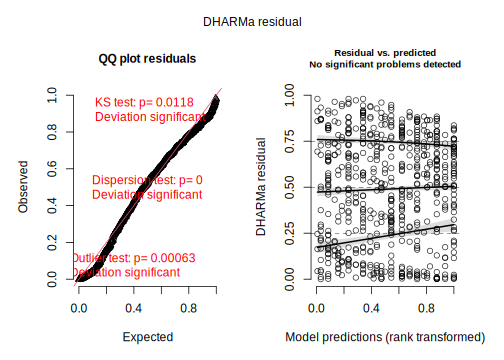
\includegraphics{BIO8940_book_files/figure-latex/unnamed-chunk-64-1.pdf}
\caption{\label{fig:unnamed-chunk-64}Distribution of BLUPs for genotypes and populations}
\end{figure}

As expected from the similarity of the variance estimates, the population-level estimates (the only shared component) do not differ much between the two models. There is a hint of regional differentiation --- the Spanish populations have higher fruit sets than the Swedish and Dutch populations. Genotype 34 again looks a little bit unusual.

\hypertarget{fixed-effects}{%
\subsubsection{Fixed effects}\label{fixed-effects}}

Now we want to do inference on the fixed effects. We use the drop1 func- tion to assess both the AIC difference and the likelihood ratio test between models. (In glmm\_funs.R we define a convenience function dfun to convert the AIC tables returned by drop1 (which we will create momentarily) into ∆AIC tables.) Although the likelihood ratio test (and the AIC) are asymptotic tests, comparing fits between full and reduced models is still more accurate than the Wald (curvature-based) tests shown in the summary tables for glmer fits.

\begin{Shaded}
\begin{Highlighting}[]
\NormalTok{(dd\_aic }\OtherTok{\textless{}{-}} \FunctionTok{dfun}\NormalTok{(}\FunctionTok{drop1}\NormalTok{(mp4)))}
\end{Highlighting}
\end{Shaded}

\begin{verbatim}
## Single term deletions
## 
## Model:
## total.fruits ~ nutrient + amd + rack + status + (1 | X) + (1 | 
##     gen) + (1 | popu) + nutrient:amd
##              npar   dAIC
## <none>             0.000
## rack            1 55.083
## status          2  1.612
## nutrient:amd    1  1.444
\end{verbatim}

\begin{Shaded}
\begin{Highlighting}[]
\NormalTok{(dd\_lrt }\OtherTok{\textless{}{-}} \FunctionTok{drop1}\NormalTok{(mp4, }\AttributeTok{test =} \StringTok{"Chisq"}\NormalTok{))}
\end{Highlighting}
\end{Shaded}

\begin{verbatim}
## Single term deletions
## 
## Model:
## total.fruits ~ nutrient + amd + rack + status + (1 | X) + (1 | 
##     gen) + (1 | popu) + nutrient:amd
##              npar    AIC    LRT   Pr(Chi)    
## <none>            5015.4                     
## rack            1 5070.5 57.083 4.179e-14 ***
## status          2 5017.0  5.612   0.06044 .  
## nutrient:amd    1 5016.8  3.444   0.06349 .  
## ---
## Signif. codes:  0 '***' 0.001 '**' 0.01 '*' 0.05 '.' 0.1 ' ' 1
\end{verbatim}

On the basis of these comparisons, there appears to be a very strong effect of rack and weak effects of status and of the interaction term. Dropping the nutrient:amd interaction gives a (slightly) increased AIC (∆AIC = 1.4), so the full model has the best expected predictive capability (by a small margin). On the other hand, the p-value is slightly above 0.05 (p = 0.06). At this point we remove the non-significant interaction term so we can test the main effects. (We don't worry about removing status because it measures an aspect of experimental design that we want to leave in the model whether it is significant or not.) Once we have fitted the reduced model, we can run the LRT via anova.

\begin{Shaded}
\begin{Highlighting}[]
\NormalTok{mp5 }\OtherTok{\textless{}{-}} \FunctionTok{update}\NormalTok{(mp4, . }\SpecialCharTok{\textasciitilde{}}\NormalTok{ . }\SpecialCharTok{{-}}\NormalTok{ amd}\SpecialCharTok{:}\NormalTok{nutrient)}
\FunctionTok{anova}\NormalTok{(mp5, mp4)}
\end{Highlighting}
\end{Shaded}

\begin{verbatim}
## Data: dat_tf
## Models:
## mp5: total.fruits ~ nutrient + amd + rack + status + (1 | X) + (1 | 
## mp5:     gen) + (1 | popu)
## mp4: total.fruits ~ nutrient + amd + rack + status + (1 | X) + (1 | 
## mp4:     gen) + (1 | popu) + nutrient:amd
##     npar    AIC    BIC  logLik deviance  Chisq Df Pr(>Chisq)  
## mp5    9 5016.8 5056.8 -2499.4   4998.8                       
## mp4   10 5015.4 5059.8 -2497.7   4995.4 3.4438  1    0.06349 .
## ---
## Signif. codes:  0 '***' 0.001 '**' 0.01 '*' 0.05 '.' 0.1 ' ' 1
\end{verbatim}

\textbf{Exercise}
Test now the reduced model.

In the reduced model, we find that both nutrients and clipping have strong effects, whether measured by AIC or LRT. If we wanted to be still more careful about our interpretation, we would try to relax the asymptotic assumption. In classical linear models, we would do this by doing F tests with the appropriate denominator degrees of freedom. In ``modern'' mixed model approaches, we might try to use denominator-degree-of-freedom approximations such as the Kenward-Roger (despite the controversy over these approximations, they are actually available in \texttt{lmerTest}, but they do not apply to GLMMs. We can use a parametric bootstrap comparison between nested models to test fixed effects, as we did above for random effects, with the caveat that is computationally slow.

In addition, we can check the normality of the random effects and find they are reasonable (Fig. 10).

\begin{Shaded}
\begin{Highlighting}[]
\NormalTok{r5 }\OtherTok{\textless{}{-}} \FunctionTok{as.data.frame}\NormalTok{(}\FunctionTok{ranef}\NormalTok{(mp5))}
\FunctionTok{ggplot}\NormalTok{(}\AttributeTok{data =}\NormalTok{ r5, }\FunctionTok{aes}\NormalTok{(}\AttributeTok{sample =}\NormalTok{ condval)) }\SpecialCharTok{+}
  \FunctionTok{geom\_qq}\NormalTok{() }\SpecialCharTok{+} \FunctionTok{geom\_qq\_line}\NormalTok{() }\SpecialCharTok{+}
  \FunctionTok{facet\_wrap}\NormalTok{(}\SpecialCharTok{\textasciitilde{}}\NormalTok{ grpvar) }\SpecialCharTok{+}
  \FunctionTok{theme\_classic}\NormalTok{()}
\end{Highlighting}
\end{Shaded}

\begin{figure}
\centering
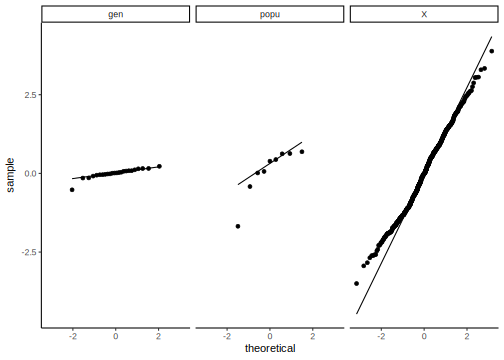
\includegraphics{BIO8940_book_files/figure-latex/unnamed-chunk-67-1.pdf}
\caption{\label{fig:unnamed-chunk-67}Q-Q plot of BLUPs from model mp5}
\end{figure}

\hypertarget{conclusions}{%
\subsection{Conclusions}\label{conclusions}}

Our final model includes fixed effects of nutrients and clipping, as well as the nuisance variables rack and status; observation-level random effects to ac- count for overdispersion; and variation in overall fruit set at the population and genotype levels. However, we don't (apparently) have quite enough in- formation to estimate the variation in clipping and nutrient effects, or their interaction, at the genotype or population levels. There is a strong overall positive effect of nutrients and a slightly weaker negative effect of clipping. The interaction between clipping and nutrients is only weakly supported (i.e.~the p-value is not very small), but it is positive and about the same magnitude as the clipping effect, which is consistent with the statement that ``nutrients cancel out the effect of herbivory''.

\begin{rmdcode}
\textbf{Exercise}

\begin{itemize}
\tightlist
\item
  Re-do the analysis with region as a fixed effect.
\item
  Re-do the analysis with a one-way layout as suggested above
\end{itemize}
\end{rmdcode}

\hypertarget{happy-generalized-mixed-modelling}{%
\section{Happy generalized mixed-modelling}\label{happy-generalized-mixed-modelling}}

\begin{figure}

{\centering \includegraphics[width=0.5\linewidth]{images/Thorn} 

}

\caption{A GLMM character}\label{fig:unnamed-chunk-69}
\end{figure}

\hypertarget{introduction-to-bayesian-inference}{%
\chapter{\texorpdfstring{Introduction to \texttt{Bayesian\ Inference}}{Introduction to Bayesian Inference}}\label{introduction-to-bayesian-inference}}

\hypertarget{theory}{%
\section{theory}\label{theory}}

\hypertarget{bayes-theorem}{%
\subsection{Bayes' theorem}\label{bayes-theorem}}

First, let's review the theorem. Mathematically, it says how to convert one conditional probability into another one.

\[ P(B \mid A) = \frac{ P(A \mid B) * P(B)}{P(A)} \]

The formula becomes more interesting in the context of statistical modeling. We
have some model that describes a data-generating process and we have some
\emph{observed} data, but we want to estimate some \emph{unknown} model parameters.
In that case, the formula reads like:

\[ P(\text{hypothesis} \mid \text{data}) = \frac{ P(\text{data} \mid \text{hypothesis}) * P(\text{hypothesis})}{P(\text{data})} \]

These terms have conventional names:

\[ \text{posterior} = \frac{ \text{likelihood} * \text{prior}}{\text{evidence}} \]

\emph{Prior} and \emph{posterior} describe when information is obtained: what we know pre-data is our
prior information, and what we learn post-data is the updated information
(``posterior'').

The \emph{likelihood} in the equation says how likely the data is given the model
parameters. I think of it as \emph{fit}: How well do the parameters fit the data?
Classical regression's line of best fit is the maximum likelihood line. The
likelihood also encompasses the data-generating process behind the model. For
example, if we assume that the observed data is normally distributed, then we
evaluate the likelihood by using the normal probability density function. You
don't need to know what that last sentence means. What's important is that the
likelihood contains our built-in assumptions about how the data is distributed.

The \emph{evidence} (sometimes called \emph{average likelihood}) is hareder to grasp. I am not sure how to describe it in an intuitive way.
It's there to make sure the math works out so that the posterior probabilities sum to 1.
Some presentations of Bayes' theorem gloss over it and I am not the exception 😄.
The important thing to note is that the posterior is proportional to the
likelihood and prior information.

\[ 
\text{posterior information} \propto 
  \text{likelihood of data} * \text{prior information} 
\]

So simply put, \textbf{you update your prior information in proportion to how well it fits
the observed data}. So essentially you are doing that on a daily basis for everything except when you ar doing frequentist stats 😄.

\begin{figure}

{\centering 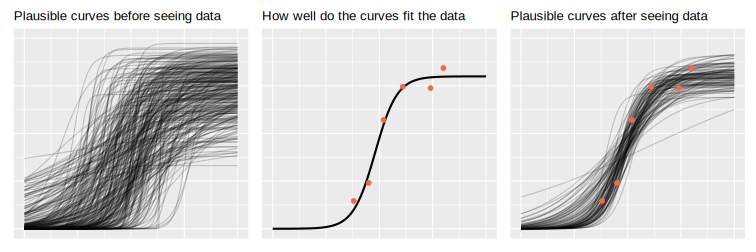
\includegraphics[width=1\linewidth]{images/bayestriptic} 

}

\caption{Bayesian Triptych}\label{fig:unnamed-chunk-71}
\end{figure}

\begin{rmdwarning}
\textbf{A word of encouragement!} The prior is an intimidating part of Bayesian
statistics. It seems highly subjective, as though we are pulling numbers from
thin air, and it can be overwhelming for complex models. But if we are familiar
with the kind of data we are modeling, we have prior information. We can have
the model simulate new observations using the prior distribution and then
plot the hypothetical data. Does anything look wrong or implausible about the
simulated data? If so, then we have some prior information that we can include
in our model. Note that we do not evaluate the plausibility of the simulated
data based on the data we have in hand (the data we want to model); that's not
prior information.
\end{rmdwarning}

\hypertarget{intro-to-mcmc}{%
\subsection{Intro to MCMC}\label{intro-to-mcmc}}

We will now walk through a simple example coded in \texttt{R} to illustrate how an MCMC algorithm works.

Suppose you are interested in the mean heart rate is of students when asked a question in a stat course. You are not sure what the exact mean value is, but you know the values are normally distributed with a standard deviation of 15. You have observed 5 individuals to have heart rate of \texttt{104,\ 120,160,90,130}. You could use MCMC sampling to draw samples from the target distribution.
We need to specify:

\begin{enumerate}
\def\labelenumi{\arabic{enumi}.}
\tightlist
\item
  the starting value for the chain.
\item
  the length of the chain. In general, more iterations will give you more accurate output.
\end{enumerate}

\begin{Shaded}
\begin{Highlighting}[]
\FunctionTok{set.seed}\NormalTok{(}\DecValTok{170}\NormalTok{)}
\NormalTok{hr\_obs }\OtherTok{\textless{}{-}} \FunctionTok{c}\NormalTok{(}\DecValTok{104}\NormalTok{, }\DecValTok{112}\NormalTok{, }\DecValTok{132}\NormalTok{, }\DecValTok{115}\NormalTok{, }\DecValTok{110}\NormalTok{)}

\NormalTok{start\_value }\OtherTok{\textless{}{-}} \DecValTok{250}

\NormalTok{n\_iter }\OtherTok{\textless{}{-}} \DecValTok{2500} \CommentTok{\# define number of iterations}

\NormalTok{pd\_mean }\OtherTok{\textless{}{-}} \FunctionTok{numeric}\NormalTok{(n\_iter) }\CommentTok{\# create vector for sample values}

\NormalTok{pd\_mean[}\DecValTok{1}\NormalTok{] }\OtherTok{\textless{}{-}}\NormalTok{ start\_value }\CommentTok{\# define starting value}

\ControlFlowTok{for}\NormalTok{ (i }\ControlFlowTok{in} \DecValTok{2}\SpecialCharTok{:}\NormalTok{n\_iter) \{}
\NormalTok{  proposal }\OtherTok{\textless{}{-}}\NormalTok{ pd\_mean[i }\SpecialCharTok{{-}} \DecValTok{1}\NormalTok{] }\SpecialCharTok{+}\NormalTok{ MASS}\SpecialCharTok{::}\FunctionTok{mvrnorm}\NormalTok{(}\DecValTok{1}\NormalTok{, }\DecValTok{0}\NormalTok{, }\DecValTok{5}\NormalTok{) }\CommentTok{\# proposal}
\NormalTok{  lprop }\OtherTok{\textless{}{-}} \FunctionTok{sum}\NormalTok{(}\FunctionTok{dnorm}\NormalTok{(proposal, hr\_obs, }\DecValTok{15}\NormalTok{)) }\CommentTok{\# likelihood of proposed parameter}
\NormalTok{  lprev }\OtherTok{\textless{}{-}} \FunctionTok{sum}\NormalTok{(}\FunctionTok{dnorm}\NormalTok{(pd\_mean[i }\SpecialCharTok{{-}} \DecValTok{1}\NormalTok{], hr\_obs, }\DecValTok{15}\NormalTok{))}
  \ControlFlowTok{if}\NormalTok{ (lprop }\SpecialCharTok{/}\NormalTok{ lprev }\SpecialCharTok{\textgreater{}} \FunctionTok{runif}\NormalTok{(}\DecValTok{1}\NormalTok{)) \{ }\CommentTok{\# if likelihood of prosposed \textgreater{} likehood previous accept }
  \CommentTok{\# and if likelihood is lower accept with random noise}
\NormalTok{    pd\_mean[i] }\OtherTok{\textless{}{-}}\NormalTok{ proposal}
\NormalTok{  \} }\CommentTok{\# if true sample the proposal}
  \ControlFlowTok{else}\NormalTok{ \{}
\NormalTok{    (pd\_mean[i] }\OtherTok{\textless{}{-}}\NormalTok{ pd\_mean[i }\SpecialCharTok{{-}} \DecValTok{1}\NormalTok{])}
\NormalTok{  \} }\CommentTok{\# if false sample the current value}
\NormalTok{\}}
\NormalTok{pd\_mean }\OtherTok{\textless{}{-}} \FunctionTok{as.mcmc}\NormalTok{(}\FunctionTok{data.frame}\NormalTok{(}\AttributeTok{mean =}\NormalTok{ pd\_mean))}
\FunctionTok{mcmc\_combo}\NormalTok{(pd\_mean, }\AttributeTok{combo =} \FunctionTok{c}\NormalTok{(}\StringTok{"trace"}\NormalTok{, }\StringTok{"dens"}\NormalTok{))}
\end{Highlighting}
\end{Shaded}

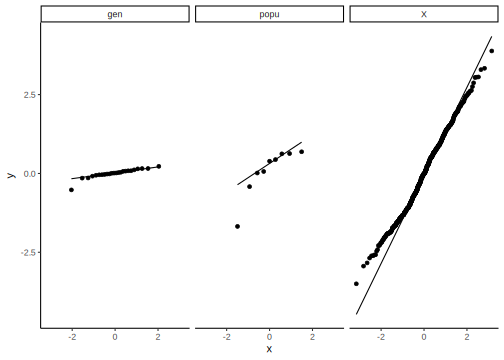
\includegraphics{BIO8940_book_files/figure-latex/unnamed-chunk-73-1.pdf}

\begin{Shaded}
\begin{Highlighting}[]
\FunctionTok{summary}\NormalTok{(pd\_mean)}
\end{Highlighting}
\end{Shaded}

\begin{verbatim}
## 
## Iterations = 1:2500
## Thinning interval = 1 
## Number of chains = 1 
## Sample size per chain = 2500 
## 
## 1. Empirical mean and standard deviation for each variable,
##    plus standard error of the mean:
## 
##           Mean             SD       Naive SE Time-series SE 
##       125.8105        32.8672         0.6573        13.3046 
## 
## 2. Quantiles for each variable:
## 
##   2.5%    25%    50%    75%  97.5% 
##  75.53 108.03 122.19 136.12 225.46
\end{verbatim}

\begin{Shaded}
\begin{Highlighting}[]
\FunctionTok{set.seed}\NormalTok{(}\DecValTok{170}\NormalTok{)}
\NormalTok{hr\_obs }\OtherTok{\textless{}{-}} \FunctionTok{c}\NormalTok{(}\DecValTok{104}\NormalTok{, }\DecValTok{112}\NormalTok{, }\DecValTok{132}\NormalTok{, }\DecValTok{115}\NormalTok{, }\DecValTok{110}\NormalTok{)}
\NormalTok{n\_iter }\OtherTok{\textless{}{-}} \DecValTok{2500} \CommentTok{\# define number of iterations}

\NormalTok{n\_chain }\OtherTok{\textless{}{-}} \DecValTok{3}
\NormalTok{start\_value }\OtherTok{\textless{}{-}} \FunctionTok{c}\NormalTok{(}\DecValTok{250}\NormalTok{, }\DecValTok{100}\NormalTok{, }\DecValTok{50}\NormalTok{)}

\NormalTok{pd\_mean }\OtherTok{\textless{}{-}} \FunctionTok{array}\NormalTok{(}\ConstantTok{NA}\NormalTok{, }\AttributeTok{dim=} \FunctionTok{c}\NormalTok{(n\_iter, n\_chain, }\DecValTok{1}\NormalTok{), }\AttributeTok{dimnames=}\FunctionTok{list}\NormalTok{(}\AttributeTok{iter =} \ConstantTok{NULL}\NormalTok{, }\AttributeTok{chain =} \ConstantTok{NULL}\NormalTok{, }\AttributeTok{params =} \StringTok{"beta"}\NormalTok{) )}\CommentTok{\# create vector for sample values}

\ControlFlowTok{for}\NormalTok{ (j }\ControlFlowTok{in} \FunctionTok{seq\_len}\NormalTok{(n\_chain)) \{}
\NormalTok{  pd\_mean[}\DecValTok{1}\NormalTok{,j,}\DecValTok{1}\NormalTok{] }\OtherTok{\textless{}{-}}\NormalTok{ start\_value[j] }\CommentTok{\# define starting value}
  \ControlFlowTok{for}\NormalTok{ (i }\ControlFlowTok{in} \DecValTok{2}\SpecialCharTok{:}\NormalTok{n\_iter) \{}
\NormalTok{    proposal }\OtherTok{\textless{}{-}}\NormalTok{ pd\_mean[i }\SpecialCharTok{{-}} \DecValTok{1}\NormalTok{, j, }\DecValTok{1}\NormalTok{] }\SpecialCharTok{+}\NormalTok{ MASS}\SpecialCharTok{::}\FunctionTok{mvrnorm}\NormalTok{(}\DecValTok{1}\NormalTok{, }\DecValTok{0}\NormalTok{, }\DecValTok{5}\NormalTok{) }\CommentTok{\# proposal}
    \ControlFlowTok{if}\NormalTok{ (}\FunctionTok{sum}\NormalTok{(}\FunctionTok{dnorm}\NormalTok{(proposal, hr\_obs, }\DecValTok{15}\NormalTok{)) }\CommentTok{\# likelihood of proposed parameter}
      \SpecialCharTok{/} \FunctionTok{sum}\NormalTok{(}\FunctionTok{dnorm}\NormalTok{(pd\_mean[i }\SpecialCharTok{{-}} \DecValTok{1}\NormalTok{, j, }\DecValTok{1}\NormalTok{], hr\_obs, }\DecValTok{15}\NormalTok{)) }\SpecialCharTok{\textgreater{}} \FunctionTok{runif}\NormalTok{(}\DecValTok{1}\NormalTok{, }\DecValTok{0}\NormalTok{, }\DecValTok{1}\NormalTok{)) \{}
\NormalTok{      pd\_mean[i, j, }\DecValTok{1}\NormalTok{] }\OtherTok{\textless{}{-}}\NormalTok{ proposal}
\NormalTok{    \} }\CommentTok{\# if true sample the proposal}
    \ControlFlowTok{else}\NormalTok{ \{}
\NormalTok{      (pd\_mean[i, j, }\DecValTok{1}\NormalTok{] }\OtherTok{\textless{}{-}}\NormalTok{ pd\_mean[i }\SpecialCharTok{{-}} \DecValTok{1}\NormalTok{, j , }\DecValTok{1}\NormalTok{])}
\NormalTok{    \} }\CommentTok{\# if false sample the current value}
\NormalTok{  \}}
\NormalTok{\}}
\FunctionTok{color\_scheme\_set}\NormalTok{(}\StringTok{"mix{-}blue{-}red"}\NormalTok{)}
\FunctionTok{mcmc\_combo}\NormalTok{(pd\_mean, }\AttributeTok{combo =} \FunctionTok{c}\NormalTok{(}\StringTok{"trace"}\NormalTok{, }\StringTok{"dens\_overlay"}\NormalTok{))}
\end{Highlighting}
\end{Shaded}

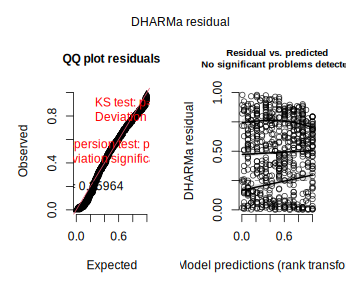
\includegraphics{BIO8940_book_files/figure-latex/unnamed-chunk-74-1.pdf}

\begin{Shaded}
\begin{Highlighting}[]
\FunctionTok{summary}\NormalTok{(pd\_mean)}
\end{Highlighting}
\end{Shaded}

\begin{verbatim}
##    Min. 1st Qu.  Median    Mean 3rd Qu.    Max. 
##   41.65   99.32  109.68  112.71  122.52  250.00
\end{verbatim}

\begin{Shaded}
\begin{Highlighting}[]
\FunctionTok{mcmc\_combo}\NormalTok{(pd\_mean, }\AttributeTok{combo =} \FunctionTok{c}\NormalTok{(}\StringTok{"trace"}\NormalTok{, }\StringTok{"dens\_overlay"}\NormalTok{), }\AttributeTok{n\_warmup =} \DecValTok{500}\NormalTok{)}
\end{Highlighting}
\end{Shaded}

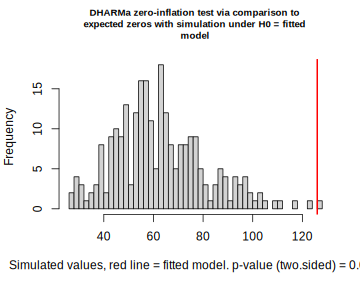
\includegraphics{BIO8940_book_files/figure-latex/unnamed-chunk-74-2.pdf}

\begin{Shaded}
\begin{Highlighting}[]
\NormalTok{pd\_burn }\OtherTok{\textless{}{-}}\NormalTok{ pd\_mean[}\SpecialCharTok{{-}}\FunctionTok{c}\NormalTok{(}\DecValTok{1}\SpecialCharTok{:}\DecValTok{500}\NormalTok{), , , drop }\OtherTok{=} \ConstantTok{FALSE}\NormalTok{]}
\FunctionTok{summary}\NormalTok{(pd\_burn)}
\end{Highlighting}
\end{Shaded}

\begin{verbatim}
##    Min. 1st Qu.  Median    Mean 3rd Qu.    Max. 
##   51.98  100.71  110.38  111.42  122.69  163.58
\end{verbatim}

\begin{Shaded}
\begin{Highlighting}[]
\FunctionTok{mcmc\_combo}\NormalTok{(pd\_burn, }\AttributeTok{combo =} \FunctionTok{c}\NormalTok{(}\StringTok{"trace"}\NormalTok{, }\StringTok{"dens\_overlay"}\NormalTok{), }\AttributeTok{iter1 =} \DecValTok{501}\NormalTok{)}
\end{Highlighting}
\end{Shaded}

\includegraphics{BIO8940_book_files/figure-latex/unnamed-chunk-74-3.pdf}

\hypertarget{inferences-1}{%
\subsection{Inferences}\label{inferences-1}}

\hypertarget{fixed-effects-1}{%
\subsubsection{Fixed effects}\label{fixed-effects-1}}

Easy peazy lemon squeezy just have a look at the posteriro distribution, does it overlap 0 yes or no.

talk about mean, median and mode of a distribution as well as credible intervals

\hypertarget{random-effects-1}{%
\subsubsection{Random effects}\label{random-effects-1}}

Quite a bit more harder. because constrained to be positive

\begin{itemize}
\tightlist
\item
  Interpreting posterior distribution
\item
  DIC
\item
  WAIC
\end{itemize}

\hypertarget{practical-4}{%
\section{Practical}\label{practical-4}}

In this practical, we will revisit our analysis on unicorn aggressivity.
Honestly, we can use any other data with repeated measures for this exercise
but I just love unicorns ❤️.
However, instead of fittng the model using \texttt{lmer()} from the \texttt{lmerTest}
📦 \citep{R-lmerTest}, we will refit the model using 2 excellent
softwares fitting models with a Bayesian approach: \texttt{MCMCglmm} \citep{MCMCglmm2010} and
\texttt{brms} \citep{R-brms}.

\hypertarget{r-packages-needed-1}{%
\subsection{R packages needed}\label{r-packages-needed-1}}

First we load required libraries

\begin{Shaded}
\begin{Highlighting}[]
\FunctionTok{library}\NormalTok{(lmerTest)}
\FunctionTok{library}\NormalTok{(tidyverse)}
\FunctionTok{library}\NormalTok{(rptR)}
\FunctionTok{library}\NormalTok{(brms)}
\FunctionTok{library}\NormalTok{(MCMCglmm)}
\FunctionTok{library}\NormalTok{(bayesplot)}
\end{Highlighting}
\end{Shaded}

\hypertarget{a-refresher-on-unicorn-ecology}{%
\subsection{A refresher on unicorn ecology}\label{a-refresher-on-unicorn-ecology}}

The last model on unicorns was:

\begin{Shaded}
\begin{Highlighting}[]
\NormalTok{aggression }\SpecialCharTok{\textasciitilde{}}\NormalTok{ opp\_size }\SpecialCharTok{+} \FunctionTok{scale}\NormalTok{(body\_size, }\AttributeTok{center =} \ConstantTok{TRUE}\NormalTok{, }\AttributeTok{scale =} \ConstantTok{TRUE}\NormalTok{)}
              \SpecialCharTok{+} \FunctionTok{scale}\NormalTok{(assay\_rep, }\AttributeTok{scale =} \ConstantTok{FALSE}\NormalTok{) }\SpecialCharTok{+}\NormalTok{ block}
              \SpecialCharTok{+}\NormalTok{ (}\DecValTok{1} \SpecialCharTok{|}\NormalTok{ ID)}
\end{Highlighting}
\end{Shaded}

Those scaled terms are abit a sore for my eyes and way too long if we need to type them multiple times in this practical.
So first let's recode them.
-

\begin{Shaded}
\begin{Highlighting}[]
\NormalTok{unicorns }\OtherTok{\textless{}{-}} \FunctionTok{read.csv}\NormalTok{(}\StringTok{"data/unicorns\_aggression.csv"}\NormalTok{)}
\NormalTok{unicorns }\OtherTok{\textless{}{-}}\NormalTok{ unicorns }\SpecialCharTok{\%\textgreater{}\%}
  \FunctionTok{mutate}\NormalTok{(}
    \AttributeTok{body\_size\_sc =} \FunctionTok{scale}\NormalTok{(body\_size),}
    \AttributeTok{assay\_rep\_sc =} \FunctionTok{scale}\NormalTok{(assay\_rep, }\AttributeTok{scale =} \ConstantTok{FALSE}\NormalTok{)}
\NormalTok{  )}
\end{Highlighting}
\end{Shaded}

Ok now we can fit the same model by just using:

\begin{Shaded}
\begin{Highlighting}[]
\NormalTok{aggression }\SpecialCharTok{\textasciitilde{}}\NormalTok{ opp\_size }\SpecialCharTok{+}\NormalTok{ body\_size\_sc }\SpecialCharTok{+}\NormalTok{ assay\_rep\_sc }\SpecialCharTok{+}\NormalTok{ block}
              \SpecialCharTok{+}\NormalTok{ (}\DecValTok{1} \SpecialCharTok{|}\NormalTok{ ID)}
\end{Highlighting}
\end{Shaded}

We can now fit a model using \texttt{lmer()}. Since we want to compare a bit \texttt{REML} and \texttt{Bayesian} aproaches, I am going to wrap the model function in a function called \texttt{system.time()}.
This function simply estimate the \texttt{user} and \texttt{computer} time use by the function.

\begin{Shaded}
\begin{Highlighting}[]
\NormalTok{mer\_time }\OtherTok{\textless{}{-}} \FunctionTok{system.time}\NormalTok{(}
\NormalTok{  m\_mer }\OtherTok{\textless{}{-}} \FunctionTok{lmer}\NormalTok{(}
\NormalTok{    aggression }\SpecialCharTok{\textasciitilde{}}\NormalTok{ opp\_size }\SpecialCharTok{+}\NormalTok{ body\_size\_sc }\SpecialCharTok{+}\NormalTok{ assay\_rep\_sc }\SpecialCharTok{+}\NormalTok{ block}
                \SpecialCharTok{+}\NormalTok{ (}\DecValTok{1} \SpecialCharTok{|}\NormalTok{ ID),}
    \AttributeTok{data =}\NormalTok{ unicorns)}
\NormalTok{)}
\NormalTok{mer\_time}
\end{Highlighting}
\end{Shaded}

\begin{verbatim}
##    user  system elapsed 
##   0.062   0.000   0.061
\end{verbatim}

\begin{Shaded}
\begin{Highlighting}[]
\FunctionTok{summary}\NormalTok{(m\_mer)}
\end{Highlighting}
\end{Shaded}

\begin{verbatim}
## Linear mixed model fit by REML. t-tests use Satterthwaite's method ['lmerModLmerTest']
## Formula: aggression ~ opp_size + body_size_sc + assay_rep_sc + block +      (1 | ID)
##    Data: unicorns
## 
## REML criterion at convergence: 1136.5
## 
## Scaled residuals: 
##      Min       1Q   Median       3Q      Max 
## -2.85473 -0.62831  0.02545  0.68998  2.74064 
## 
## Random effects:
##  Groups   Name        Variance Std.Dev.
##  ID       (Intercept) 0.02538  0.1593  
##  Residual             0.58048  0.7619  
## Number of obs: 480, groups:  ID, 80
## 
## Fixed effects:
##               Estimate Std. Error        df t value Pr(>|t|)    
## (Intercept)    9.00181    0.03907  78.07315 230.395   <2e-16 ***
## opp_size       1.05141    0.04281 396.99857  24.562   <2e-16 ***
## body_size_sc   0.03310    0.03896  84.21144   0.850    0.398    
## assay_rep_sc  -0.05783    0.04281 396.99857  -1.351    0.177    
## block         -0.02166    0.06955 397.00209  -0.311    0.756    
## ---
## Signif. codes:  0 '***' 0.001 '**' 0.01 '*' 0.05 '.' 0.1 ' ' 1
## 
## Correlation of Fixed Effects:
##             (Intr) opp_sz bdy_s_ assy__
## opp_size     0.000                     
## body_siz_sc  0.000  0.000              
## assay_rp_sc  0.000 -0.100  0.000       
## block        0.000  0.000  0.002  0.000
\end{verbatim}

Ok so it took no time at all to do it and we got our ``classic'' results.

\hypertarget{mcmcglmm}{%
\subsection{MCMCglmm}\label{mcmcglmm}}

What makes \texttt{MCMCglmm} so useful and powerful 💪 in ecology and for \emph{practical Bayesian people} is that:

\begin{enumerate}
\def\labelenumi{\arabic{enumi}.}
\tightlist
\item
  it is blazing fast ⏩ (for Bayesian analysis) for some models particularly models with structured covariances
\item
  it is fairly intuitive to code
\end{enumerate}

\textbf{but} it also has some inconvenients:

\begin{enumerate}
\def\labelenumi{\arabic{enumi}.}
\tightlist
\item
  it is blazing fast for \textbf{Bayesian analysis} meaning it is 🐌 compared to \emph{maximum likelihood} approaches
\item
  it has some limitations in terms of functionality, distribution availability and model specifications compared to other \emph{Bayesian} softwares
\item
  the priors, \emph{oh, the priors} 😭, are a bit tricky to code and understand 🤯.
\end{enumerate}

\hypertarget{fitting-the-model}{%
\subsubsection{Fitting the Model}\label{fitting-the-model}}

So here is how we can code the model in \texttt{MCMCglmm()}. It is fairly similar to \texttt{lmer()} except that the random effects are specified in a different \emph{argument}.

\begin{Shaded}
\begin{Highlighting}[]
\NormalTok{mcglm\_time }\OtherTok{\textless{}{-}} \FunctionTok{system.time}\NormalTok{(}
\NormalTok{  m\_mcmcglmm }\OtherTok{\textless{}{-}} \FunctionTok{MCMCglmm}\NormalTok{(}
\NormalTok{    aggression }\SpecialCharTok{\textasciitilde{}}\NormalTok{ opp\_size }\SpecialCharTok{+}\NormalTok{ body\_size\_sc }\SpecialCharTok{+}\NormalTok{ assay\_rep\_sc }\SpecialCharTok{+}\NormalTok{ block,}
                \AttributeTok{random =} \SpecialCharTok{\textasciitilde{}}\NormalTok{ ID,}
    \AttributeTok{data =}\NormalTok{ unicorns)}
\NormalTok{)}
\end{Highlighting}
\end{Shaded}

\begin{verbatim}
## 
##                        MCMC iteration = 0
## 
##                        MCMC iteration = 1000
## 
##                        MCMC iteration = 2000
## 
##                        MCMC iteration = 3000
## 
##                        MCMC iteration = 4000
## 
##                        MCMC iteration = 5000
## 
##                        MCMC iteration = 6000
## 
##                        MCMC iteration = 7000
## 
##                        MCMC iteration = 8000
## 
##                        MCMC iteration = 9000
## 
##                        MCMC iteration = 10000
## 
##                        MCMC iteration = 11000
## 
##                        MCMC iteration = 12000
## 
##                        MCMC iteration = 13000
\end{verbatim}

\begin{Shaded}
\begin{Highlighting}[]
\FunctionTok{summary}\NormalTok{(m\_mcmcglmm)}
\end{Highlighting}
\end{Shaded}

\begin{verbatim}
## 
##  Iterations = 3001:12991
##  Thinning interval  = 10
##  Sample size  = 1000 
## 
##  DIC: 1128.004 
## 
##  G-structure:  ~ID
## 
##    post.mean  l-95% CI u-95% CI eff.samp
## ID  0.003686 9.807e-14   0.0262    45.81
## 
##  R-structure:  ~units
## 
##       post.mean l-95% CI u-95% CI eff.samp
## units    0.6044   0.5228   0.6819     1000
## 
##  Location effects: aggression ~ opp_size + body_size_sc + assay_rep_sc + block 
## 
##              post.mean l-95% CI u-95% CI eff.samp  pMCMC    
## (Intercept)    9.00152  8.93150  9.07158     1000 <0.001 ***
## opp_size       1.04940  0.96813  1.12946     1000 <0.001 ***
## body_size_sc   0.03154 -0.03985  0.09563     1000  0.410    
## assay_rep_sc  -0.05620 -0.13196  0.03546      893  0.184    
## block         -0.02069 -0.16186  0.11553     1000  0.774    
## ---
## Signif. codes:  0 '***' 0.001 '**' 0.01 '*' 0.05 '.' 0.1 ' ' 1
\end{verbatim}

\begin{Shaded}
\begin{Highlighting}[]
\NormalTok{mcglm\_time}
\end{Highlighting}
\end{Shaded}

\begin{verbatim}
##    user  system elapsed 
##   2.850   0.000   2.851
\end{verbatim}

Model is slow and not good. We need more iteration and maybe even a longer burnin, and honestly maybe better priors.

\begin{Shaded}
\begin{Highlighting}[]
\FunctionTok{plot}\NormalTok{(m\_mcmcglmm}\SpecialCharTok{$}\NormalTok{Sol)}
\end{Highlighting}
\end{Shaded}

\includegraphics{BIO8940_book_files/figure-latex/unnamed-chunk-78-1.pdf} 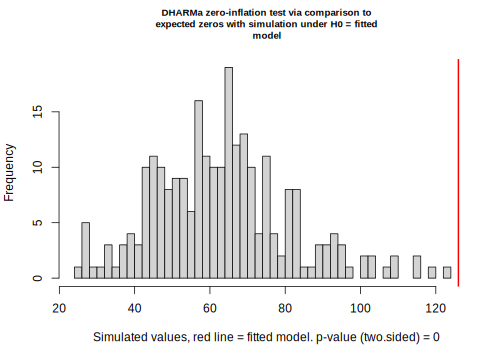
\includegraphics{BIO8940_book_files/figure-latex/unnamed-chunk-78-2.pdf}

\begin{Shaded}
\begin{Highlighting}[]
\FunctionTok{plot}\NormalTok{(m\_mcmcglmm}\SpecialCharTok{$}\NormalTok{VCV)}
\end{Highlighting}
\end{Shaded}

\begin{figure}
\centering
\includegraphics{BIO8940_book_files/figure-latex/unnamed-chunk-78-3.pdf}
\caption{\label{fig:unnamed-chunk-78-3}Posterior trace and distribution of the paremeters in m\_mcmcglmm using default settings}
\end{figure}

\begin{Shaded}
\begin{Highlighting}[]
\FunctionTok{autocorr.diag}\NormalTok{(m\_mcmcglmm}\SpecialCharTok{$}\NormalTok{VCV)}
\end{Highlighting}
\end{Shaded}

\begin{verbatim}
##                ID       units
## Lag 0   1.0000000  1.00000000
## Lag 10  0.8042405 -0.02074155
## Lag 50  0.4807583 -0.04264317
## Lag 100 0.1951356  0.04422296
## Lag 500 0.1254589  0.04401956
\end{verbatim}

Talk about autocorrelation, mixing, convergence and priors here

\begin{Shaded}
\begin{Highlighting}[]
\NormalTok{n\_samp }\OtherTok{\textless{}{-}} \DecValTok{1000}
\NormalTok{thin }\OtherTok{\textless{}{-}} \DecValTok{500}
\NormalTok{burnin }\OtherTok{\textless{}{-}} \DecValTok{20000}
\NormalTok{mcglm\_time }\OtherTok{\textless{}{-}} \FunctionTok{system.time}\NormalTok{(}
\NormalTok{  m\_mcmcglmm }\OtherTok{\textless{}{-}} \FunctionTok{MCMCglmm}\NormalTok{(}
\NormalTok{    aggression }\SpecialCharTok{\textasciitilde{}}\NormalTok{ opp\_size }\SpecialCharTok{+}\NormalTok{ body\_size\_sc }\SpecialCharTok{+}\NormalTok{ assay\_rep\_sc }\SpecialCharTok{+}\NormalTok{ block,}
                \AttributeTok{random =} \SpecialCharTok{\textasciitilde{}}\NormalTok{ ID,}
    \AttributeTok{data =}\NormalTok{ unicorns,}
    \AttributeTok{nitt =}\NormalTok{ n\_samp }\SpecialCharTok{*}\NormalTok{ thin }\SpecialCharTok{+}\NormalTok{ burnin, }\AttributeTok{thin =}\NormalTok{ thin, }\AttributeTok{burnin =}\NormalTok{ burnin,}
    \AttributeTok{verbose =} \ConstantTok{FALSE}\NormalTok{,}
    \AttributeTok{prior =} \FunctionTok{list}\NormalTok{(}
      \AttributeTok{R =} \FunctionTok{list}\NormalTok{(}\AttributeTok{V =} \DecValTok{1}\NormalTok{, }\AttributeTok{nu =} \FloatTok{0.002}\NormalTok{),}
      \AttributeTok{G =} \FunctionTok{list}\NormalTok{(}
        \AttributeTok{G1 =} \FunctionTok{list}\NormalTok{(}\AttributeTok{V =} \DecValTok{1}\NormalTok{, }\AttributeTok{nu =} \FloatTok{0.002}\NormalTok{)}
\NormalTok{      )}
\NormalTok{    )}
\NormalTok{  )}
\NormalTok{)}
\FunctionTok{summary}\NormalTok{(m\_mcmcglmm)}
\end{Highlighting}
\end{Shaded}

\begin{verbatim}
## 
##  Iterations = 20001:519501
##  Thinning interval  = 500
##  Sample size  = 1000 
## 
##  DIC: 1126.66 
## 
##  G-structure:  ~ID
## 
##    post.mean  l-95% CI u-95% CI eff.samp
## ID   0.01987 0.0002904  0.05458     1000
## 
##  R-structure:  ~units
## 
##       post.mean l-95% CI u-95% CI eff.samp
## units    0.5917   0.5188   0.6763     1000
## 
##  Location effects: aggression ~ opp_size + body_size_sc + assay_rep_sc + block 
## 
##              post.mean l-95% CI u-95% CI eff.samp  pMCMC    
## (Intercept)    9.00136  8.92221  9.07383     1000 <0.001 ***
## opp_size       1.05363  0.96382  1.13650     1000 <0.001 ***
## body_size_sc   0.03373 -0.03781  0.10686     1000  0.396    
## assay_rep_sc  -0.05861 -0.14186  0.02882     1000  0.182    
## block         -0.02709 -0.16061  0.11441     1000  0.698    
## ---
## Signif. codes:  0 '***' 0.001 '**' 0.01 '*' 0.05 '.' 0.1 ' ' 1
\end{verbatim}

\begin{Shaded}
\begin{Highlighting}[]
\NormalTok{mcglm\_time}
\end{Highlighting}
\end{Shaded}

\begin{verbatim}
##    user  system elapsed 
##  78.058   0.003  78.069
\end{verbatim}

evaluate model here

\begin{Shaded}
\begin{Highlighting}[]
\FunctionTok{plot}\NormalTok{(m\_mcmcglmm}\SpecialCharTok{$}\NormalTok{Sol)}
\end{Highlighting}
\end{Shaded}

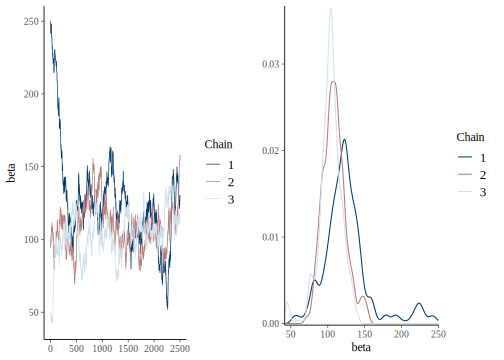
\includegraphics{BIO8940_book_files/figure-latex/unnamed-chunk-80-1.pdf} \includegraphics{BIO8940_book_files/figure-latex/unnamed-chunk-80-2.pdf}

\begin{Shaded}
\begin{Highlighting}[]
\FunctionTok{plot}\NormalTok{(m\_mcmcglmm}\SpecialCharTok{$}\NormalTok{VCV)}
\end{Highlighting}
\end{Shaded}

\begin{figure}
\centering
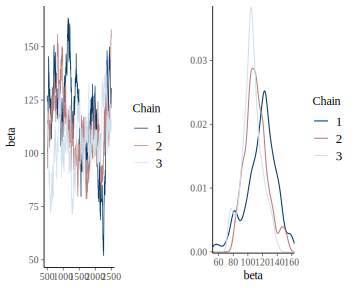
\includegraphics{BIO8940_book_files/figure-latex/unnamed-chunk-80-3.pdf}
\caption{\label{fig:unnamed-chunk-80-3}Posterior trace and distribution of the paremeters in m\_mcmcglmm with better settings}
\end{figure}

\begin{Shaded}
\begin{Highlighting}[]
\FunctionTok{autocorr.diag}\NormalTok{(m\_mcmcglmm}\SpecialCharTok{$}\NormalTok{VCV)}
\end{Highlighting}
\end{Shaded}

\begin{verbatim}
##                     ID        units
## Lag 0      1.000000000  1.000000000
## Lag 500    0.013876043 -0.044235206
## Lag 2500   0.026120260 -0.048012241
## Lag 5000  -0.049357725  0.021158672
## Lag 25000  0.002544256 -0.003722595
\end{verbatim}

\hypertarget{inferences-2}{%
\subsection{Inferences}\label{inferences-2}}

\hypertarget{fixed-effects-2}{%
\subsubsection{Fixed effects}\label{fixed-effects-2}}

Easy peazy lemon squeezy just have a look at the posteriro distribution, does it overlap 0 yes or no.

\begin{Shaded}
\begin{Highlighting}[]
\FunctionTok{posterior.mode}\NormalTok{(m\_mcmcglmm}\SpecialCharTok{$}\NormalTok{Sol)}
\end{Highlighting}
\end{Shaded}

\begin{verbatim}
##  (Intercept)     opp_size body_size_sc assay_rep_sc        block 
##   9.00632282   1.07353252   0.03500916  -0.04048582  -0.03276275
\end{verbatim}

\begin{Shaded}
\begin{Highlighting}[]
\FunctionTok{HPDinterval}\NormalTok{(m\_mcmcglmm}\SpecialCharTok{$}\NormalTok{Sol)}
\end{Highlighting}
\end{Shaded}

\begin{verbatim}
##                    lower      upper
## (Intercept)   8.92221005 9.07383400
## opp_size      0.96382086 1.13649873
## body_size_sc -0.03781276 0.10685606
## assay_rep_sc -0.14185602 0.02882443
## block        -0.16060691 0.11440706
## attr(,"Probability")
## [1] 0.95
\end{verbatim}

\hypertarget{random-effects-2}{%
\subsubsection{Random effects}\label{random-effects-2}}

Quite a bit more harder. because constrained to be positive

\begin{Shaded}
\begin{Highlighting}[]
\FunctionTok{posterior.mode}\NormalTok{(m\_mcmcglmm}\SpecialCharTok{$}\NormalTok{VCV)}
\end{Highlighting}
\end{Shaded}

\begin{verbatim}
##         ID      units 
## 0.00096263 0.59129362
\end{verbatim}

\begin{Shaded}
\begin{Highlighting}[]
\FunctionTok{HPDinterval}\NormalTok{(m\_mcmcglmm}\SpecialCharTok{$}\NormalTok{VCV)}
\end{Highlighting}
\end{Shaded}

\begin{verbatim}
##              lower      upper
## ID    0.0002903938 0.05458376
## units 0.5188238599 0.67634529
## attr(,"Probability")
## [1] 0.95
\end{verbatim}

\hypertarget{brms}{%
\subsection{brms}\label{brms}}

\textbf{brms} is an acronym for \emph{Bayesian Regression Models using `Stan'} \citep{R-brms}. It is a package developed to fit regression models with a Bayesian approach using the amazing \texttt{stan} software \citep{stan2021}.

What makes \texttt{brms} so useful and powerful 💪 in ecology is that:

\begin{enumerate}
\def\labelenumi{\arabic{enumi}.}
\tightlist
\item
  it is really intuitive to code (same syntax as \texttt{glmer()})
\item
  it is incredibly flexible since it is essentially a front end for \texttt{stan} via its \texttt{rstan} interface \citep{R-rstan}
\end{enumerate}

\textbf{but} with \emph{great powers come great responsability} 🕷

\begin{Shaded}
\begin{Highlighting}[]
\NormalTok{brm\_time }\OtherTok{\textless{}{-}} \FunctionTok{system.time}\NormalTok{(}
\NormalTok{  m\_brm }\OtherTok{\textless{}{-}} \FunctionTok{brm}\NormalTok{(}
\NormalTok{    aggression }\SpecialCharTok{\textasciitilde{}}\NormalTok{ opp\_size }\SpecialCharTok{+}\NormalTok{ body\_size\_sc }\SpecialCharTok{+}\NormalTok{ assay\_rep\_sc }\SpecialCharTok{+}\NormalTok{ block}
        \SpecialCharTok{+}\NormalTok{ (}\DecValTok{1} \SpecialCharTok{|}\NormalTok{ ID),}
    \AttributeTok{data =}\NormalTok{ unicorns, }\AttributeTok{iter =} \DecValTok{4750}\NormalTok{, }\AttributeTok{warmup =} \DecValTok{1000}\NormalTok{, }\AttributeTok{thin =} \DecValTok{15}\NormalTok{, }\AttributeTok{cores =}\DecValTok{4}
    \CommentTok{\#refresh = 0}
\NormalTok{  )}
\NormalTok{)}
\end{Highlighting}
\end{Shaded}

\begin{verbatim}
## Compiling Stan program...
\end{verbatim}

\begin{verbatim}
## Start sampling
\end{verbatim}

\begin{Shaded}
\begin{Highlighting}[]
\NormalTok{brm\_time}
\end{Highlighting}
\end{Shaded}

\begin{verbatim}
##    user  system elapsed 
##   7.423   1.381  18.031
\end{verbatim}

\begin{Shaded}
\begin{Highlighting}[]
\FunctionTok{summary}\NormalTok{(m\_brm)}
\end{Highlighting}
\end{Shaded}

\begin{verbatim}
##  Family: gaussian 
##   Links: mu = identity; sigma = identity 
## Formula: aggression ~ opp_size + body_size_sc + assay_rep_sc + block + (1 | ID) 
##    Data: unicorns (Number of observations: 480) 
## Samples: 4 chains, each with iter = 4750; warmup = 1000; thin = 15;
##          total post-warmup samples = 1000
## 
## Group-Level Effects: 
## ~ID (Number of levels: 80) 
##               Estimate Est.Error l-95% CI u-95% CI Rhat Bulk_ESS Tail_ESS
## sd(Intercept)     0.14      0.07     0.01     0.27 1.00      940      899
## 
## Population-Level Effects: 
##              Estimate Est.Error l-95% CI u-95% CI Rhat Bulk_ESS Tail_ESS
## Intercept        9.00      0.04     8.93     9.07 1.00     1098      871
## opp_size         1.05      0.04     0.97     1.13 1.00     1057     1035
## body_size_sc     0.03      0.04    -0.04     0.11 1.00     1069      918
## assay_rep_sc    -0.06      0.04    -0.14     0.02 1.00      956      781
## block           -0.02      0.07    -0.16     0.12 1.00      963      955
## 
## Family Specific Parameters: 
##       Estimate Est.Error l-95% CI u-95% CI Rhat Bulk_ESS Tail_ESS
## sigma     0.77      0.03     0.72     0.83 1.00      990      882
## 
## Samples were drawn using sampling(NUTS). For each parameter, Bulk_ESS
## and Tail_ESS are effective sample size measures, and Rhat is the potential
## scale reduction factor on split chains (at convergence, Rhat = 1).
\end{verbatim}

\begin{Shaded}
\begin{Highlighting}[]
\FunctionTok{mcmc\_acf\_bar}\NormalTok{(m\_brm, }\AttributeTok{regex\_pars =} \FunctionTok{c}\NormalTok{(}\StringTok{"sd"}\NormalTok{))}
\end{Highlighting}
\end{Shaded}

\begin{figure}
\centering
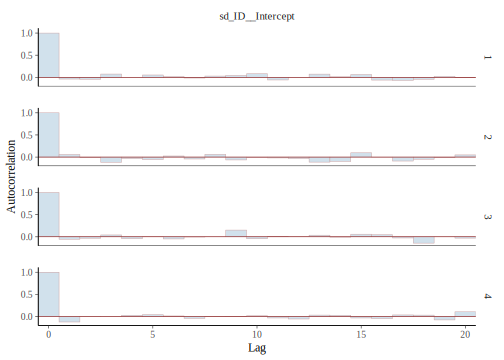
\includegraphics{BIO8940_book_files/figure-latex/unnamed-chunk-83-1.pdf}
\caption{\label{fig:unnamed-chunk-83}Autocorrelation in the chain for variance parameters in model m\_brm}
\end{figure}

\hypertarget{hunder-the-hood}{%
\subsubsection{Hunder the hood}\label{hunder-the-hood}}

have a look at the \texttt{stan} code

\begin{Shaded}
\begin{Highlighting}[]
\FunctionTok{stancode}\NormalTok{(m\_brm)}
\end{Highlighting}
\end{Shaded}

\begin{verbatim}
## // generated with brms 2.14.4
## functions {
## }
## data {
##   int<lower=1> N;  // total number of observations
##   vector[N] Y;  // response variable
##   int<lower=1> K;  // number of population-level effects
##   matrix[N, K] X;  // population-level design matrix
##   // data for group-level effects of ID 1
##   int<lower=1> N_1;  // number of grouping levels
##   int<lower=1> M_1;  // number of coefficients per level
##   int<lower=1> J_1[N];  // grouping indicator per observation
##   // group-level predictor values
##   vector[N] Z_1_1;
##   int prior_only;  // should the likelihood be ignored?
## }
## transformed data {
##   int Kc = K - 1;
##   matrix[N, Kc] Xc;  // centered version of X without an intercept
##   vector[Kc] means_X;  // column means of X before centering
##   for (i in 2:K) {
##     means_X[i - 1] = mean(X[, i]);
##     Xc[, i - 1] = X[, i] - means_X[i - 1];
##   }
## }
## parameters {
##   vector[Kc] b;  // population-level effects
##   real Intercept;  // temporary intercept for centered predictors
##   real<lower=0> sigma;  // residual SD
##   vector<lower=0>[M_1] sd_1;  // group-level standard deviations
##   vector[N_1] z_1[M_1];  // standardized group-level effects
## }
## transformed parameters {
##   vector[N_1] r_1_1;  // actual group-level effects
##   r_1_1 = (sd_1[1] * (z_1[1]));
## }
## model {
##   // likelihood including all constants
##   if (!prior_only) {
##     // initialize linear predictor term
##     vector[N] mu = Intercept + rep_vector(0.0, N);
##     for (n in 1:N) {
##       // add more terms to the linear predictor
##       mu[n] += r_1_1[J_1[n]] * Z_1_1[n];
##     }
##     target += normal_id_glm_lpdf(Y | Xc, mu, b, sigma);
##   }
##   // priors including all constants
##   target += student_t_lpdf(Intercept | 3, 8.9, 2.5);
##   target += student_t_lpdf(sigma | 3, 0, 2.5)
##     - 1 * student_t_lccdf(0 | 3, 0, 2.5);
##   target += student_t_lpdf(sd_1 | 3, 0, 2.5)
##     - 1 * student_t_lccdf(0 | 3, 0, 2.5);
##   target += std_normal_lpdf(z_1[1]);
## }
## generated quantities {
##   // actual population-level intercept
##   real b_Intercept = Intercept - dot_product(means_X, b);
## }
\end{verbatim}

\hypertarget{using-shiny}{%
\subsubsection{using shiny}\label{using-shiny}}

\begin{Shaded}
\begin{Highlighting}[]
\FunctionTok{launch\_shinystan}\NormalTok{(m\_brm)}
\end{Highlighting}
\end{Shaded}

\begin{figure}

{\centering \includegraphics[width=0.5\linewidth]{images/shinystan} 

}

\caption{Shinystan interface}\label{fig:unnamed-chunk-86}
\end{figure}

\hypertarget{inferences-3}{%
\subsection{Inferences}\label{inferences-3}}

\hypertarget{fixed-effects-3}{%
\subsubsection{Fixed effects}\label{fixed-effects-3}}

\begin{Shaded}
\begin{Highlighting}[]
\FunctionTok{summary}\NormalTok{(m\_brm)}
\end{Highlighting}
\end{Shaded}

\begin{verbatim}
##  Family: gaussian 
##   Links: mu = identity; sigma = identity 
## Formula: aggression ~ opp_size + body_size_sc + assay_rep_sc + block + (1 | ID) 
##    Data: unicorns (Number of observations: 480) 
## Samples: 4 chains, each with iter = 4750; warmup = 1000; thin = 15;
##          total post-warmup samples = 1000
## 
## Group-Level Effects: 
## ~ID (Number of levels: 80) 
##               Estimate Est.Error l-95% CI u-95% CI Rhat Bulk_ESS Tail_ESS
## sd(Intercept)     0.14      0.07     0.01     0.27 1.00      940      899
## 
## Population-Level Effects: 
##              Estimate Est.Error l-95% CI u-95% CI Rhat Bulk_ESS Tail_ESS
## Intercept        9.00      0.04     8.93     9.07 1.00     1098      871
## opp_size         1.05      0.04     0.97     1.13 1.00     1057     1035
## body_size_sc     0.03      0.04    -0.04     0.11 1.00     1069      918
## assay_rep_sc    -0.06      0.04    -0.14     0.02 1.00      956      781
## block           -0.02      0.07    -0.16     0.12 1.00      963      955
## 
## Family Specific Parameters: 
##       Estimate Est.Error l-95% CI u-95% CI Rhat Bulk_ESS Tail_ESS
## sigma     0.77      0.03     0.72     0.83 1.00      990      882
## 
## Samples were drawn using sampling(NUTS). For each parameter, Bulk_ESS
## and Tail_ESS are effective sample size measures, and Rhat is the potential
## scale reduction factor on split chains (at convergence, Rhat = 1).
\end{verbatim}

\begin{Shaded}
\begin{Highlighting}[]
\FunctionTok{mcmc\_plot}\NormalTok{(m\_brm, }\AttributeTok{regex\_pars =} \StringTok{"b\_"}\NormalTok{)}
\end{Highlighting}
\end{Shaded}

\begin{figure}
\centering
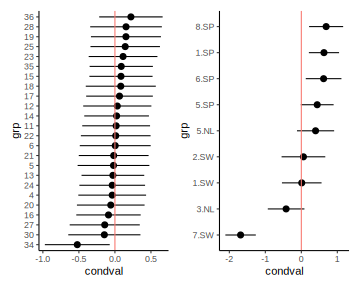
\includegraphics{BIO8940_book_files/figure-latex/unnamed-chunk-87-1.pdf}
\caption{\label{fig:unnamed-chunk-87}Fixed effect estimates (with 95\% credible intervals) from model m\_brm}
\end{figure}

\hypertarget{random-effects-3}{%
\subsubsection{Random effects}\label{random-effects-3}}

\begin{Shaded}
\begin{Highlighting}[]
\FunctionTok{summary}\NormalTok{(m\_brm)}
\end{Highlighting}
\end{Shaded}

\begin{verbatim}
##  Family: gaussian 
##   Links: mu = identity; sigma = identity 
## Formula: aggression ~ opp_size + body_size_sc + assay_rep_sc + block + (1 | ID) 
##    Data: unicorns (Number of observations: 480) 
## Samples: 4 chains, each with iter = 4750; warmup = 1000; thin = 15;
##          total post-warmup samples = 1000
## 
## Group-Level Effects: 
## ~ID (Number of levels: 80) 
##               Estimate Est.Error l-95% CI u-95% CI Rhat Bulk_ESS Tail_ESS
## sd(Intercept)     0.14      0.07     0.01     0.27 1.00      940      899
## 
## Population-Level Effects: 
##              Estimate Est.Error l-95% CI u-95% CI Rhat Bulk_ESS Tail_ESS
## Intercept        9.00      0.04     8.93     9.07 1.00     1098      871
## opp_size         1.05      0.04     0.97     1.13 1.00     1057     1035
## body_size_sc     0.03      0.04    -0.04     0.11 1.00     1069      918
## assay_rep_sc    -0.06      0.04    -0.14     0.02 1.00      956      781
## block           -0.02      0.07    -0.16     0.12 1.00      963      955
## 
## Family Specific Parameters: 
##       Estimate Est.Error l-95% CI u-95% CI Rhat Bulk_ESS Tail_ESS
## sigma     0.77      0.03     0.72     0.83 1.00      990      882
## 
## Samples were drawn using sampling(NUTS). For each parameter, Bulk_ESS
## and Tail_ESS are effective sample size measures, and Rhat is the potential
## scale reduction factor on split chains (at convergence, Rhat = 1).
\end{verbatim}

\begin{Shaded}
\begin{Highlighting}[]
\FunctionTok{mcmc\_plot}\NormalTok{(m\_brm, }\AttributeTok{pars =} \FunctionTok{c}\NormalTok{(}\StringTok{"sd\_ID\_\_Intercept"}\NormalTok{, }\StringTok{"sigma"}\NormalTok{))}
\end{Highlighting}
\end{Shaded}

\begin{figure}
\centering
\includegraphics{BIO8940_book_files/figure-latex/unnamed-chunk-88-1.pdf}
\caption{\label{fig:unnamed-chunk-88}Among-individual and residual standard deviance ( with 95\% credible intervals) estimated from model m\_brm}
\end{figure}

\hypertarget{happy-bayesian-stats}{%
\section{Happy Bayesian stats}\label{happy-bayesian-stats}}

\begin{figure}

{\centering \includegraphics[width=0.5\linewidth]{images/sherlock} 

}

\caption{Sherlock Holmes, a truly bayesian detective}\label{fig:unnamed-chunk-89}
\end{figure}

\hypertarget{random-regressions-and-multivariate-mixed-models}{%
\chapter{Random regressions and multivariate mixed models}\label{random-regressions-and-multivariate-mixed-models}}

\hypertarget{theory-1}{%
\section{theory}\label{theory-1}}

Amazing beasties and crazy animals

\begin{figure}

{\centering \includegraphics[width=0.5\linewidth]{images/fun_dragon} 

}

\caption{Dream pet dragon}\label{fig:unnamed-chunk-90}
\end{figure}

\hypertarget{practical-5}{%
\section{Practical}\label{practical-5}}

In this practical, we have collected data on the amazing blue dragon of the west that roam the sky at night.

We will use two different 📦 to fit more complex models that are not possible with \texttt{lmer()} from \texttt{lme4}
📦 \citep{R-lme4}. We will use:

\begin{itemize}
\tightlist
\item
  \texttt{asreml-R} which is a commercial software developped by VSNi \citep{R-asreml}. \texttt{ASReml} fit models using a maxiumum likelihood approach, is quite flexible and fast.
\item
  \texttt{MCMCglmm} which is free and open-source and fit model using a Bayesian approach \citep{MCMCglmm2010}. It is super flexible and allow to fit a wide diversity of distribution.
\end{itemize}

The aims of the practical are to learn:

\begin{itemize}
\tightlist
\item
  How to phrase questions of interest in terms of variances and covariances (or derived correlations or regressions);
\item
  How to incorporate more advanced model structures, such as:

  \begin{itemize}
  \tightlist
  \item
    Fixed effects that apply only to a subset of the response traits;
  \item
    Traits which are measured a different number of times (e.g., repeated measures of behaviour and a single value of breeding success);
  \end{itemize}
\item
  Hypothesis testing using likelihood ratio tests.
\end{itemize}

\hypertarget{r-packages-needed-2}{%
\subsection{R packages needed}\label{r-packages-needed-2}}

First we load required libraries

\begin{Shaded}
\begin{Highlighting}[]
\FunctionTok{library}\NormalTok{(lmerTest)}
\FunctionTok{library}\NormalTok{(tidyverse)}
\FunctionTok{library}\NormalTok{(asreml)}
\FunctionTok{library}\NormalTok{(MCMCglmm)}
\FunctionTok{library}\NormalTok{(nadiv)}
\end{Highlighting}
\end{Shaded}

\hypertarget{the-blue-dragon-of-the-west}{%
\subsection{The blue dragon of the west}\label{the-blue-dragon-of-the-west}}

For this practical, we have collected data on the amazing blue dragon of the west that roam the sky at night.

\begin{figure}

{\centering \includegraphics[width=0.5\linewidth]{images/blue_dragon} 

}

\caption{Blue dragon male}\label{fig:unnamed-chunk-91}
\end{figure}

We tagged all dragons individually when they hatch from their eggs. Here, we concentrate on female dragon that produce a single clucth of eggs per mating seasons. Adult femlae blue dragons need to explore vast amount of land to find a compatible male. We thus hypothesized that maximum flight speed as well as exploration are key traits to determine fitness. We were able to obtain repeated measures of flying speed and exploration on 80 adult females during one mating season and also measure the number of egg layed at the end of the season.

Each females was capture 4 times during the season and each time we measured the maximum flying speed using a wind tunnel and exploration using a openfield test.

The data frame has 6 variables:

\begin{itemize}
\tightlist
\item
  ID: Individual identity
\item
  assay\_rep: the repeat number of the behavioural assay
\item
  max\_speed: maximum flying speed
\item
  exploration:
\item
  eggs: measure of reproductive succes measured only once per individual
\item
  body\_size: individual body size measured on the day of the test
\end{itemize}

\begin{Shaded}
\begin{Highlighting}[]
\NormalTok{df\_dragons }\OtherTok{\textless{}{-}} \FunctionTok{read.csv}\NormalTok{(}\StringTok{"data/dragons.csv"}\NormalTok{)}
\FunctionTok{str}\NormalTok{(df\_dragons)}
\end{Highlighting}
\end{Shaded}

\begin{verbatim}
## 'data.frame':    320 obs. of  6 variables:
##  $ ID         : chr  "S_1" "S_1" "S_1" "S_1" ...
##  $ assay_rep  : int  1 2 3 4 1 2 3 4 1 2 ...
##  $ max_speed  : num  58.7 57.9 64.3 61.4 65.5 ...
##  $ exploration: num  126 125 127 127 125 ...
##  $ eggs       : int  39 NA NA NA 56 NA NA NA 51 NA ...
##  $ body_size  : num  21.7 21.5 21.3 20.8 25.7 ...
\end{verbatim}

To help with convergence of the model, and also help with parameter interpretation, we will first scale our covariates.

\begin{Shaded}
\begin{Highlighting}[]
\NormalTok{df\_dragons }\OtherTok{\textless{}{-}}\NormalTok{ df\_dragons }\SpecialCharTok{\%\textgreater{}\%}
  \FunctionTok{mutate}\NormalTok{(}
    \AttributeTok{body\_size\_sc =} \FunctionTok{scale}\NormalTok{(body\_size),}
    \AttributeTok{assay\_rep\_sc =} \FunctionTok{scale}\NormalTok{(assay\_rep, }\AttributeTok{scale =} \ConstantTok{FALSE}\NormalTok{)}
\NormalTok{  )}
\end{Highlighting}
\end{Shaded}

\hypertarget{multiple-univariate-models}{%
\subsection{Multiple univariate models}\label{multiple-univariate-models}}

We first use the \texttt{lme4} 📦 to determine the proportion of phenotypic variation (adjusted for fixed effects) that is due to differences among individuals, separately for each trait with repeated measures.

\hypertarget{flying-speed}{%
\subsubsection{Flying speed}\label{flying-speed}}

Our model includes fixed effects of the assay repeat number (centred) and individual body size (centred and scaled to standard deviation units), as we wish to control for any systematic effects of these variables on individual behaviour. Be aware that controlling variables are at your discretion --- for example, while we want to characterise among-individual variance in flying speed after controlling for size effects in this study, others may wish to characterise among-individual variance in flying speed without such control. Using techniques shown later in the practical, it would be entirely possible to characterise both among-individual variance in flying speed and in size, and the among-individual covariance between these measurements.

\begin{Shaded}
\begin{Highlighting}[]
\NormalTok{lmer\_f }\OtherTok{\textless{}{-}} \FunctionTok{lmer}\NormalTok{(max\_speed }\SpecialCharTok{\textasciitilde{}}\NormalTok{ assay\_rep\_sc }\SpecialCharTok{+}\NormalTok{ body\_size\_sc }\SpecialCharTok{+}\NormalTok{ (}\DecValTok{1} \SpecialCharTok{|}\NormalTok{ ID),}
  \AttributeTok{data =}\NormalTok{ df\_dragons}
\NormalTok{)}
\FunctionTok{par}\NormalTok{(}\AttributeTok{mfrow =} \FunctionTok{c}\NormalTok{(}\DecValTok{1}\NormalTok{, }\DecValTok{3}\NormalTok{))}
\FunctionTok{plot}\NormalTok{(}\FunctionTok{resid}\NormalTok{(lmer\_f, }\AttributeTok{type =} \StringTok{"pearson"}\NormalTok{) }\SpecialCharTok{\textasciitilde{}} \FunctionTok{fitted}\NormalTok{(lmer\_f))}
\FunctionTok{qqnorm}\NormalTok{(}\FunctionTok{residuals}\NormalTok{(lmer\_f))}
\FunctionTok{qqline}\NormalTok{(}\FunctionTok{residuals}\NormalTok{(lmer\_f))}
\FunctionTok{hist}\NormalTok{(}\FunctionTok{residuals}\NormalTok{(lmer\_f))}
\end{Highlighting}
\end{Shaded}

\begin{figure}
\centering
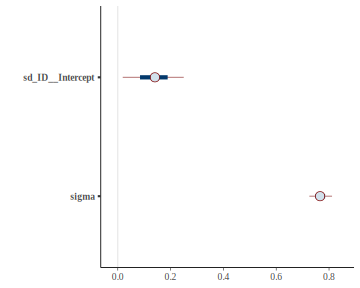
\includegraphics{BIO8940_book_files/figure-latex/unnamed-chunk-94-1.pdf}
\caption{\label{fig:unnamed-chunk-94}Checking assumptions of model lmer\_f}
\end{figure}

\begin{Shaded}
\begin{Highlighting}[]
\FunctionTok{summary}\NormalTok{(lmer\_f)}
\end{Highlighting}
\end{Shaded}

\begin{verbatim}
## Linear mixed model fit by REML. t-tests use Satterthwaite's method ['lmerModLmerTest']
## Formula: max_speed ~ assay_rep_sc + body_size_sc + (1 | ID)
##    Data: df_dragons
## 
## REML criterion at convergence: 1791.4
## 
## Scaled residuals: 
##     Min      1Q  Median      3Q     Max 
## -2.3645 -0.6496 -0.1154  0.6463  2.6894 
## 
## Random effects:
##  Groups   Name        Variance Std.Dev.
##  ID       (Intercept)  6.951   2.636   
##  Residual             11.682   3.418   
## Number of obs: 320, groups:  ID, 80
## 
## Fixed effects:
##              Estimate Std. Error       df t value Pr(>|t|)    
## (Intercept)   63.5344     0.3513  78.0954 180.870   <2e-16 ***
## assay_rep_sc  -0.1519     0.1709 238.9807  -0.889    0.375    
## body_size_sc   0.4468     0.3445  88.0328   1.297    0.198    
## ---
## Signif. codes:  0 '***' 0.001 '**' 0.01 '*' 0.05 '.' 0.1 ' ' 1
## 
## Correlation of Fixed Effects:
##             (Intr) assy__
## assay_rp_sc  0.000       
## body_siz_sc  0.000 -0.002
\end{verbatim}

Having examined diagnostic plots of the model fit, we can check the model summary. We are interested in the random effects section of the lme4 model output (specifically the variance component --- note that the standard deviation here is simply the square root of the variance). Evidence for `animal personality' (or `consistent among-individual differences in behaviour') in the literature is largely taken from the repeatability of behaviorual traits: we can compute this repeatability (also known as the intraclass correlation coefficient) by dividing the variance in the trait due to differences among individuals (\(V_{ID}\)) by the total phenotypic variance after accounting for the fixed effects (\(V_{ID} + V_{residual}\) ).

\begin{Shaded}
\begin{Highlighting}[]
\NormalTok{rep\_flying }\OtherTok{\textless{}{-}} \FunctionTok{as.data.frame}\NormalTok{(}\FunctionTok{VarCorr}\NormalTok{(lmer\_f)) }\SpecialCharTok{\%\textgreater{}\%}
  \FunctionTok{select}\NormalTok{(grp, vcov) }\SpecialCharTok{\%\textgreater{}\%}
  \FunctionTok{spread}\NormalTok{(grp, vcov) }\SpecialCharTok{\%\textgreater{}\%}
  \FunctionTok{mutate}\NormalTok{(}\AttributeTok{repeatability =}\NormalTok{ ID }\SpecialCharTok{/}\NormalTok{ (ID }\SpecialCharTok{+}\NormalTok{ Residual))}
\NormalTok{rep\_flying}
\end{Highlighting}
\end{Shaded}

\begin{table}

\caption{\label{tab:unnamed-chunk-96}Variance components and repeatbility for the maximum
   flying speed of blue dragons}
\centering
\begin{tabular}[t]{r|r|r}
\hline
ID & Residual & repeatability\\
\hline
6.951 & 11.682 & 0.373\\
\hline
\end{tabular}
\end{table}

So we can see that 37.31\% of the phenotypic variation in boldness (having controlled for body size and assay
repeat number) is due to differences among individuals.

\hypertarget{exploration}{%
\subsubsection{Exploration}\label{exploration}}

\begin{Shaded}
\begin{Highlighting}[]
\NormalTok{lmer\_e }\OtherTok{\textless{}{-}} \FunctionTok{lmer}\NormalTok{(exploration }\SpecialCharTok{\textasciitilde{}}\NormalTok{ assay\_rep\_sc }\SpecialCharTok{+}\NormalTok{ body\_size\_sc }\SpecialCharTok{+}\NormalTok{ (}\DecValTok{1} \SpecialCharTok{|}\NormalTok{ ID),}
  \AttributeTok{data =}\NormalTok{ df\_dragons}
\NormalTok{)}
\FunctionTok{par}\NormalTok{(}\AttributeTok{mfrow =} \FunctionTok{c}\NormalTok{(}\DecValTok{1}\NormalTok{, }\DecValTok{3}\NormalTok{))}
\FunctionTok{plot}\NormalTok{(}\FunctionTok{resid}\NormalTok{(lmer\_e, }\AttributeTok{type =} \StringTok{"pearson"}\NormalTok{) }\SpecialCharTok{\textasciitilde{}} \FunctionTok{fitted}\NormalTok{(lmer\_e))}
\FunctionTok{qqnorm}\NormalTok{(}\FunctionTok{residuals}\NormalTok{(lmer\_e))}
\FunctionTok{qqline}\NormalTok{(}\FunctionTok{residuals}\NormalTok{(lmer\_e))}
\FunctionTok{hist}\NormalTok{(}\FunctionTok{residuals}\NormalTok{(lmer\_e))}
\end{Highlighting}
\end{Shaded}

\begin{figure}
\centering
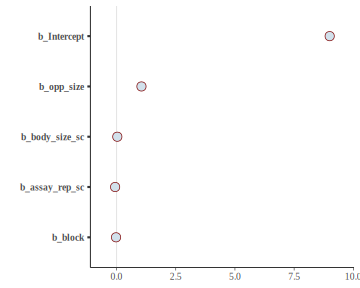
\includegraphics{BIO8940_book_files/figure-latex/unnamed-chunk-97-1.pdf}
\caption{\label{fig:unnamed-chunk-97}Checking assumptions of model lmer\_e}
\end{figure}

\begin{Shaded}
\begin{Highlighting}[]
\FunctionTok{summary}\NormalTok{(lmer\_e)}
\end{Highlighting}
\end{Shaded}

\begin{verbatim}
## Linear mixed model fit by REML. t-tests use Satterthwaite's method ['lmerModLmerTest']
## Formula: exploration ~ assay_rep_sc + body_size_sc + (1 | ID)
##    Data: df_dragons
## 
## REML criterion at convergence: 1691.2
## 
## Scaled residuals: 
##      Min       1Q   Median       3Q      Max 
## -2.73290 -0.62520  0.01635  0.55523  2.95896 
## 
## Random effects:
##  Groups   Name        Variance Std.Dev.
##  ID       (Intercept) 3.623    1.903   
##  Residual             9.091    3.015   
## Number of obs: 320, groups:  ID, 80
## 
## Fixed effects:
##               Estimate Std. Error        df t value Pr(>|t|)    
## (Intercept)  127.22524    0.27148  78.08871 468.639   <2e-16 ***
## assay_rep_sc  -0.07811    0.15076 238.99943  -0.518    0.605    
## body_size_sc   0.26114    0.26806  85.68180   0.974    0.333    
## ---
## Signif. codes:  0 '***' 0.001 '**' 0.01 '*' 0.05 '.' 0.1 ' ' 1
## 
## Correlation of Fixed Effects:
##             (Intr) assy__
## assay_rp_sc  0.000       
## body_siz_sc  0.000 -0.002
\end{verbatim}

So the model looks good and we can see our estimates for both fixed and random effects. We can now estimate the repeatbility of exploration.

\begin{Shaded}
\begin{Highlighting}[]
\NormalTok{rep\_expl }\OtherTok{\textless{}{-}} \FunctionTok{as.data.frame}\NormalTok{(}\FunctionTok{VarCorr}\NormalTok{(lmer\_e)) }\SpecialCharTok{\%\textgreater{}\%}
  \FunctionTok{select}\NormalTok{(grp, vcov) }\SpecialCharTok{\%\textgreater{}\%}
  \FunctionTok{spread}\NormalTok{(grp, vcov) }\SpecialCharTok{\%\textgreater{}\%}
  \FunctionTok{mutate}\NormalTok{(}\AttributeTok{repeatability =}\NormalTok{ ID }\SpecialCharTok{/}\NormalTok{ (ID }\SpecialCharTok{+}\NormalTok{ Residual))}
\NormalTok{rep\_expl}
\end{Highlighting}
\end{Shaded}

\begin{table}

\caption{\label{tab:unnamed-chunk-99}Variance components and repeatability for exploration
   behaviour of blue dragons}
\centering
\begin{tabular}[t]{r|r|r}
\hline
ID & Residual & repeatability\\
\hline
6.951 & 11.682 & 0.373\\
\hline
\end{tabular}
\end{table}

Both of traits of interest are repeatable at the among-individual level. So, the remaining question is estimating the relation between these two traits. Are individuals that are consistently faster than average also more exploratory than average (and vice versa)?

\hypertarget{correlation-using-blups}{%
\subsubsection{Correlation using BLUPs}\label{correlation-using-blups}}

Using BLUPs to estimate correlations between traits or to further investigate biological associations can lead to spurious results and anticonservative hypothesis tests and narrow confidence intervals. \citet{hadfield_misuse_2010} discuss the problem as well as present some alternative method to avoid the problem using Bayesian methods. However, it is always preferable to use multivariate models when possible.

We need to create a data frame that contain the BLUPs from both univariate models.

\begin{Shaded}
\begin{Highlighting}[]
\NormalTok{df\_blups\_fe }\OtherTok{\textless{}{-}} \FunctionTok{merge}\NormalTok{(}
  \FunctionTok{as.data.frame}\NormalTok{(}\FunctionTok{ranef}\NormalTok{(lmer\_f)),}
  \FunctionTok{as.data.frame}\NormalTok{(}\FunctionTok{ranef}\NormalTok{(lmer\_e)),}
  \AttributeTok{by =} \StringTok{"grp"}
\NormalTok{) }\SpecialCharTok{\%\textgreater{}\%}
  \FunctionTok{mutate}\NormalTok{(}
    \AttributeTok{speed =}\NormalTok{ condval.x,}
    \AttributeTok{exploration =}\NormalTok{ condval.y}
\NormalTok{  )}
\end{Highlighting}
\end{Shaded}

We can now test the correlation among-individual between flying speed and exploration.

\begin{Shaded}
\begin{Highlighting}[]
\NormalTok{(cor\_blups }\OtherTok{\textless{}{-}} \FunctionTok{with}\NormalTok{(df\_blups\_fe, }\FunctionTok{cor.test}\NormalTok{(condval.x, condval.y)))}
\end{Highlighting}
\end{Shaded}

\begin{verbatim}
## 
##  Pearson's product-moment correlation
## 
## data:  condval.x and condval.y
## t = 3.2131, df = 78, p-value = 0.00191
## alternative hypothesis: true correlation is not equal to 0
## 95 percent confidence interval:
##  0.1320924 0.5223645
## sample estimates:
##       cor 
## 0.3418867
\end{verbatim}

\begin{Shaded}
\begin{Highlighting}[]
\FunctionTok{ggplot}\NormalTok{(df\_blups\_fe, }\FunctionTok{aes}\NormalTok{(}\AttributeTok{x =}\NormalTok{ exploration, }\AttributeTok{y =}\NormalTok{ speed)) }\SpecialCharTok{+}
  \FunctionTok{geom\_point}\NormalTok{() }\SpecialCharTok{+}
  \FunctionTok{labs}\NormalTok{(}\AttributeTok{xlab =} \StringTok{"Exploration (BLUP)"}\NormalTok{, }\AttributeTok{ylab =} \StringTok{"Flying speed (BLUP)"}\NormalTok{) }\SpecialCharTok{+}
  \FunctionTok{theme\_classic}\NormalTok{()}
\end{Highlighting}
\end{Shaded}

\begin{figure}
\centering
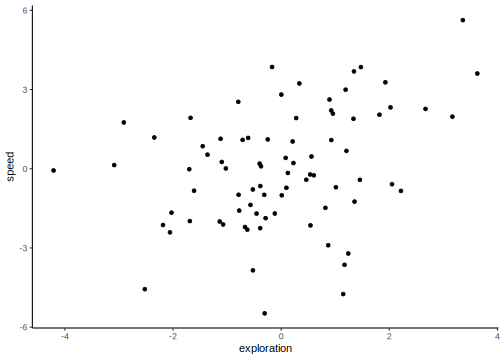
\includegraphics{BIO8940_book_files/figure-latex/unnamed-chunk-101-1.pdf}
\caption{\label{fig:unnamed-chunk-101}Relation between exploration and flying speed using BLUPs from univariate models}
\end{figure}

As you can see, we get a positive correlation with a very small p-value (\(P = 0.0019099\)), indicating that these traits are involved in a behavioural syndrome. While the correlation itself is fairly weak (\$r = 0.3418867), it appears to be highly significant, and suggests that individuals that are faster than average also tend to be more exploratory than average.
However, as discussed in \citet{hadfield_misuse_2010} and \citet{houslay_avoiding_2017}, using BLUPs in this way leads to anticonservative significance tests. This is because the error inherent in their prediction is not carried forward from the lmer models to the subsequent analysis (in this case, a correlation test).
To illustrate this point quickly, below we plot the individual estimates along with their associated standard errors.

\begin{Shaded}
\begin{Highlighting}[]
\FunctionTok{ggplot}\NormalTok{(df\_blups\_fe, }\FunctionTok{aes}\NormalTok{(}\AttributeTok{x =}\NormalTok{ exploration, }\AttributeTok{y =}\NormalTok{ speed)) }\SpecialCharTok{+}
  \FunctionTok{geom\_point}\NormalTok{() }\SpecialCharTok{+}
  \FunctionTok{geom\_linerange}\NormalTok{(}\FunctionTok{aes}\NormalTok{(}
    \AttributeTok{xmin =}\NormalTok{ exploration }\SpecialCharTok{{-}}\NormalTok{ condsd.x,}
    \AttributeTok{xmax =}\NormalTok{ exploration }\SpecialCharTok{+}\NormalTok{ condsd.x}
\NormalTok{  )) }\SpecialCharTok{+}
  \FunctionTok{geom\_linerange}\NormalTok{(}\FunctionTok{aes}\NormalTok{(}
    \AttributeTok{ymin =}\NormalTok{ speed }\SpecialCharTok{{-}}\NormalTok{ condsd.y,}
    \AttributeTok{ymax =}\NormalTok{ speed }\SpecialCharTok{+}\NormalTok{ condsd.y}
\NormalTok{  )) }\SpecialCharTok{+}
  \FunctionTok{labs}\NormalTok{(}
    \AttributeTok{xlab =} \StringTok{"Exploration (BLUP +/{-} SE)"}\NormalTok{,}
    \AttributeTok{ylab =} \StringTok{"Flying speed (BLUP +/{-} SE)"}
\NormalTok{  ) }\SpecialCharTok{+}
  \FunctionTok{theme\_classic}\NormalTok{()}
\end{Highlighting}
\end{Shaded}

\begin{figure}
\centering
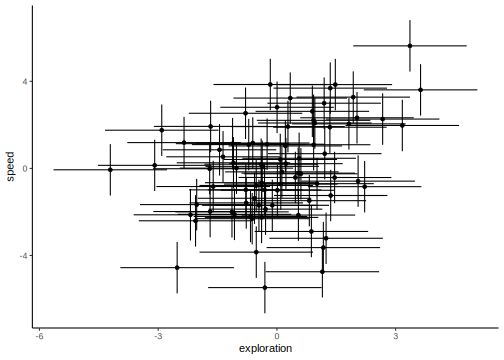
\includegraphics{BIO8940_book_files/figure-latex/unnamed-chunk-102-1.pdf}
\caption{\label{fig:unnamed-chunk-102}Relation between exploration and flying speed using BLUPs from univariate models including +/- SE as error bars}
\end{figure}

\hypertarget{multivariate-approach}{%
\subsection{Multivariate approach}\label{multivariate-approach}}

\hypertarget{based-on-asremlr}{%
\subsubsection{Based on ASRemlR}\label{based-on-asremlr}}

The correct approach for testing the hypothesised relation between speed and exploration uses both response variables in a two-trait (`bivariate') mixed model. This model estimates the among-individual variance for each response variable (and the covariance between them).
Separate (co)variances are also fitted for the residual variation.
The bivariate model also allows for fixed effects to be fitted on both response variables.
We set up our model using the \texttt{asreml} function call, with our bivariate response variable being \texttt{exploration} and flying \texttt{speed} bound together using \texttt{cbind}. You will also note that we scale our response variables, meaning that each is centred at their mean value and standardised to units of 1 standard deviation. This is not essential, but simply makes it easier for the model to be fit. Scaling the response variables also aids our understanding of the output, as both flying speed and exploration are now on the same scale.

\texttt{asreml} can be a bit specific sometime and random effects should absolutely be \texttt{factor} and not \texttt{character} or \texttt{integer}

\begin{Shaded}
\begin{Highlighting}[]
\NormalTok{df\_dragons }\OtherTok{\textless{}{-}}\NormalTok{ df\_dragons }\SpecialCharTok{\%\textgreater{}\%}
  \FunctionTok{mutate}\NormalTok{(}
    \AttributeTok{ID =} \FunctionTok{as.factor}\NormalTok{(ID),}
    \AttributeTok{speed\_sc =} \FunctionTok{scale}\NormalTok{(max\_speed),}
    \AttributeTok{exploration\_sc =} \FunctionTok{scale}\NormalTok{(exploration)}
\NormalTok{  )}

\NormalTok{asr\_us }\OtherTok{\textless{}{-}} \FunctionTok{asreml}\NormalTok{(}\FunctionTok{cbind}\NormalTok{(speed\_sc, exploration\_sc) }\SpecialCharTok{\textasciitilde{}}\NormalTok{ trait }\SpecialCharTok{+}
\NormalTok{  trait}\SpecialCharTok{:}\NormalTok{assay\_rep\_sc }\SpecialCharTok{+}\NormalTok{ trait}\SpecialCharTok{:}\NormalTok{body\_size\_sc,}
\AttributeTok{random =} \SpecialCharTok{\textasciitilde{}}\NormalTok{ ID}\SpecialCharTok{:}\FunctionTok{us}\NormalTok{(trait),}
\AttributeTok{residual =} \SpecialCharTok{\textasciitilde{}}\NormalTok{ units}\SpecialCharTok{:}\FunctionTok{us}\NormalTok{(trait),}
\AttributeTok{data =}\NormalTok{ df\_dragons,}
\AttributeTok{maxiter =} \DecValTok{100}
\NormalTok{)}
\end{Highlighting}
\end{Shaded}

\begin{verbatim}
## Model fitted using the sigma parameterization.
## ASReml 4.1.0 Fri Mar 19 23:53:13 2021
##           LogLik        Sigma2     DF     wall    cpu
##  1      -333.105           1.0    634 23:53:13    0.0
##  2      -303.637           1.0    634 23:53:13    0.0
##  3      -274.849           1.0    634 23:53:13    0.0
##  4      -260.243           1.0    634 23:53:13    0.0
##  5      -256.118           1.0    634 23:53:13    0.0
##  6      -255.891           1.0    634 23:53:13    0.0
##  7      -255.889           1.0    634 23:53:13    0.0
\end{verbatim}

On the right hand side of our model formula, we use the \texttt{trait} keyword to specify that this is a multivariate model --- \texttt{trait} itself tells the model to give us the intercept for each trait. We then interact \texttt{trait} with the fixed effects, \texttt{assay\_rep\_sc} and \texttt{body\_size\_sc}, so that we get estimates for the effect of these variables on each of teh 2 traits.
The random effects structure starts with the random effects, where we tell the model to fit an \emph{unstructured} (us) covariance matrix for the grouping variable ID. This means that the variance in exploration due to differences among individuals, the variance in boldness due to differences among individuals, and the covariance between these variances will be estimated.
Next, we set a structure for the residual variation (\texttt{residual}), which is also sometimes known as the \emph{within-individual variation}. As we have repeated measures for both traits at the individual level, we also set an \emph{unstructured} covariance matrix, which estimates the residual variance for each trait and also allows the residuals
to covary across the two traits.
Finally, we provide the name of the data frame, and a maximum number of iterations for ASReml to attempt to fit the model.
After the model has been fit by ASReml, we can check the fit using the same type of model diagnostic plots as we use for \texttt{lme4}:

\begin{Shaded}
\begin{Highlighting}[]
\FunctionTok{par}\NormalTok{(}\AttributeTok{mfrow =} \FunctionTok{c}\NormalTok{(}\DecValTok{1}\NormalTok{, }\DecValTok{3}\NormalTok{))}
\FunctionTok{plot}\NormalTok{(}\FunctionTok{residuals}\NormalTok{(asr\_us) }\SpecialCharTok{\textasciitilde{}} \FunctionTok{fitted}\NormalTok{(asr\_us))}
\FunctionTok{qqnorm}\NormalTok{(}\FunctionTok{residuals}\NormalTok{(asr\_us))}
\FunctionTok{qqline}\NormalTok{(}\FunctionTok{residuals}\NormalTok{(asr\_us))}
\FunctionTok{hist}\NormalTok{(}\FunctionTok{residuals}\NormalTok{(asr\_us))}
\end{Highlighting}
\end{Shaded}

\begin{figure}
\centering
\includegraphics{BIO8940_book_files/figure-latex/unnamed-chunk-104-1.pdf}
\caption{\label{fig:unnamed-chunk-104}Checking assumptions of model asr\_us}
\end{figure}

The summary part of the ASReml model fit contains a large amount of information, so it is best to look only at certain parts of it at a single time. While we are not particularly interested in the fixed effects for current purposes, you can inspect these using the following code to check whether there were any large effects of \texttt{assay\ repeat} or \texttt{body\ size} on either trait:

\begin{Shaded}
\begin{Highlighting}[]
\FunctionTok{summary}\NormalTok{(asr\_us, }\AttributeTok{all =} \ConstantTok{TRUE}\NormalTok{)}\SpecialCharTok{$}\NormalTok{coef.fixed}
\end{Highlighting}
\end{Shaded}

\begin{verbatim}
## NULL
\end{verbatim}

We can see that there is a separate intercept for both personality traits (no surprise that these are very close to zero, given that we mean-centred and scaled each trait before fitting the model), and an estimate of the effect of assay repeat and body size on both traits. None of these appear to be large effects, so let's move on to the more interesting parts --- the random effects estimates:

\begin{Shaded}
\begin{Highlighting}[]
\FunctionTok{summary}\NormalTok{(asr\_us)}\SpecialCharTok{$}\NormalTok{varcomp}
\end{Highlighting}
\end{Shaded}

\begin{verbatim}
##                                                  component  std.error   z.ratio bound %ch
## ID:trait!trait_speed_sc:speed_sc                0.37333063 0.08607123  4.337461     P   0
## ID:trait!trait_exploration_sc:speed_sc          0.08838639 0.06067006  1.456837     P   0
## ID:trait!trait_exploration_sc:exploration_sc    0.28631012 0.07637247  3.748865     P   0
## units:trait!R                                   1.00000000         NA        NA     F   0
## units:trait!trait_speed_sc:speed_sc             0.62741689 0.05740281 10.930073     P   0
## units:trait!trait_exploration_sc:speed_sc       0.32632113 0.04829175  6.757286     P   0
## units:trait!trait_exploration_sc:exploration_sc 0.71844189 0.06572780 10.930563     P   0
\end{verbatim}

In the above summary table, we have the among-individual (co)variances listed first (starting with ID), then the residual (or within-individual) (co)variances (starting with R). You will notice that the variance estimates here are actually close to the \texttt{lme4} repeatability estimates, because our response variables were scaled to phenotypic standard deviations. We can also find the `adjusted repeatability' (i.e., the repeatability conditional on the fixed effects) for each trait by dividing its among-individual variance estimate by the sum
of its among-individual and residual variances.
Here, we use the \texttt{vpredict} function to estimate the repeatability and its
standard error for each trait, conditional on the effects of assay repeat and body size.
For this function, we provide the name of the model object, followed by a name that we want to give the estimate being returned, and a formula for the calculation. Each `V' term in the formula refers to a variance component, using its position in the model summary shown above.

\begin{Shaded}
\begin{Highlighting}[]
\FunctionTok{vpredict}\NormalTok{(asr\_us, rep\_speed }\SpecialCharTok{\textasciitilde{}}\NormalTok{ V1 }\SpecialCharTok{/}\NormalTok{ (V1 }\SpecialCharTok{+}\NormalTok{ V5))}
\end{Highlighting}
\end{Shaded}

\begin{verbatim}
##            Estimate         SE
## rep_speed 0.3730518 0.06124032
\end{verbatim}

\begin{Shaded}
\begin{Highlighting}[]
\FunctionTok{vpredict}\NormalTok{(asr\_us, rep\_expl }\SpecialCharTok{\textasciitilde{}}\NormalTok{ V3 }\SpecialCharTok{/}\NormalTok{ (V3 }\SpecialCharTok{+}\NormalTok{ V7))}
\end{Highlighting}
\end{Shaded}

\begin{verbatim}
##          Estimate         SE
## rep_expl 0.284956 0.06113539
\end{verbatim}

We can also use this function to calculate the estimate and standard error of the correlation from our model (co)variances. We do this by specifying the formula for the correlation:

\begin{Shaded}
\begin{Highlighting}[]
\NormalTok{(cor\_fe }\OtherTok{\textless{}{-}} \FunctionTok{vpredict}\NormalTok{(asr\_us, rep\_expl }\SpecialCharTok{\textasciitilde{}}\NormalTok{ V2 }\SpecialCharTok{/}\NormalTok{ (}\FunctionTok{sqrt}\NormalTok{(V1 }\SpecialCharTok{*}\NormalTok{ V3))))}
\end{Highlighting}
\end{Shaded}

\begin{verbatim}
##           Estimate        SE
## rep_expl 0.2703462 0.1594097
\end{verbatim}

In this case, the estimate is similar (here, slightly lower) than our correlation estimate using BLUPs.
However, if we consider confidence intervals as \(+/- 1.96SE\) around the estimate, the lower bound of the confidence interval would actually be -0.0420968024949831.
With confidence intervals straddling zero, we would conclude that this correlation is likely non-significant.
As the use of standard errors in this way is only approximate, we should also test our hypothesis formally using likelihood ratio tests.

\hypertarget{hypothesis-testing}{%
\paragraph{Hypothesis testing}\label{hypothesis-testing}}

We can now test the statistical significance of this correlation directly, by fitting a second model without the among-individual covariance between our two traits, and then using a likelihood ratio test to determine whether the model with the covariance produces a better fit.
Here, we use the \texttt{idh} structure for our random effects. This stands for `identity matrix' (i.e., with 0s on the off-diagonals) with heterogeneous variances (i.e., the variance components for our two response traits are allowed to be different from one another).
The rest of the model is identical to the previous version.

\begin{Shaded}
\begin{Highlighting}[]
\NormalTok{asr\_us }\OtherTok{\textless{}{-}} \FunctionTok{asreml}\NormalTok{(}\FunctionTok{cbind}\NormalTok{(speed\_sc, exploration\_sc) }\SpecialCharTok{\textasciitilde{}}\NormalTok{ trait }\SpecialCharTok{+}
\NormalTok{  trait}\SpecialCharTok{:}\NormalTok{assay\_rep\_sc }\SpecialCharTok{+}\NormalTok{ trait}\SpecialCharTok{:}\NormalTok{body\_size\_sc,}
\AttributeTok{random =} \SpecialCharTok{\textasciitilde{}}\NormalTok{ ID}\SpecialCharTok{:}\FunctionTok{idh}\NormalTok{(trait),}
\AttributeTok{residual =} \SpecialCharTok{\textasciitilde{}}\NormalTok{ units}\SpecialCharTok{:}\FunctionTok{us}\NormalTok{(trait),}
\AttributeTok{data =}\NormalTok{ df\_dragons,}
\AttributeTok{maxiter =} \DecValTok{100}
\NormalTok{)}
\end{Highlighting}
\end{Shaded}

\begin{verbatim}
## Model fitted using the sigma parameterization.
## ASReml 4.1.0 Fri Mar 19 23:53:14 2021
##           LogLik        Sigma2     DF     wall    cpu
##  1      -327.051           1.0    634 23:53:14    0.0
##  2      -299.874           1.0    634 23:53:14    0.0
##  3      -273.689           1.0    634 23:53:14    0.0
##  4      -260.838           1.0    634 23:53:14    0.0
##  5      -257.331           1.0    634 23:53:14    0.0
##  6      -257.120           1.0    634 23:53:14    0.0
##  7      -257.118           1.0    634 23:53:14    0.0
\end{verbatim}

The likelihood ratio test is calculated as twice the difference between model log-likelihoods, on a single degree of freedom (the covariance term):

\begin{Shaded}
\begin{Highlighting}[]
\NormalTok{(p\_biv }\OtherTok{\textless{}{-}} \FunctionTok{pchisq}\NormalTok{(}\DecValTok{2} \SpecialCharTok{*}\NormalTok{ (asr\_us}\SpecialCharTok{$}\NormalTok{loglik }\SpecialCharTok{{-}}\NormalTok{ asr\_us}\SpecialCharTok{$}\NormalTok{loglik),}
  \AttributeTok{df =} \DecValTok{1}\NormalTok{,}
  \AttributeTok{lower.tail =} \ConstantTok{FALSE}
\NormalTok{))}
\end{Highlighting}
\end{Shaded}

\begin{verbatim}
## [1] 1
\end{verbatim}

In sharp contrast to the highly-significant P-value given by a correlation test using BLUPs, here we find no evidence for a correlation between flying speed and exploration.
To better understand why BLUPs produce an anticonservative p-value in comparison to multivariate models, we should plot the correlation estimates and their confidence intervals. The confidence intervals are taken directly from the cor.test function for BLUPs, and for ASReml they are calculated as 1.96 times the standard error from the \texttt{vpredict} function.

\begin{Shaded}
\begin{Highlighting}[]
\NormalTok{df\_cor }\OtherTok{\textless{}{-}} \FunctionTok{data.frame}\NormalTok{(}
  \AttributeTok{Method =} \FunctionTok{c}\NormalTok{(}\StringTok{"ASReml"}\NormalTok{, }\StringTok{"BLUPs"}\NormalTok{),}
  \AttributeTok{Correlation =} \FunctionTok{c}\NormalTok{(}\FunctionTok{as.numeric}\NormalTok{(cor\_fe[}\DecValTok{1}\NormalTok{]), cor\_blups}\SpecialCharTok{$}\NormalTok{estimate),}
  \AttributeTok{low =} \FunctionTok{c}\NormalTok{(}\FunctionTok{as.numeric}\NormalTok{(cor\_fe[}\DecValTok{1}\NormalTok{] }\SpecialCharTok{{-}} \FloatTok{1.96} \SpecialCharTok{*}\NormalTok{ cor\_fe[}\DecValTok{2}\NormalTok{]), cor\_blups}\SpecialCharTok{$}\NormalTok{conf.int[}\DecValTok{1}\NormalTok{]),}
  \AttributeTok{high =} \FunctionTok{c}\NormalTok{(}\FunctionTok{as.numeric}\NormalTok{(cor\_fe[}\DecValTok{1}\NormalTok{] }\SpecialCharTok{+} \FloatTok{1.96} \SpecialCharTok{*}\NormalTok{ cor\_fe[}\DecValTok{2}\NormalTok{]), cor\_blups}\SpecialCharTok{$}\NormalTok{conf.int[}\DecValTok{2}\NormalTok{])}
\NormalTok{)}
\FunctionTok{ggplot}\NormalTok{(df\_cor, }\FunctionTok{aes}\NormalTok{(}\AttributeTok{x =}\NormalTok{ Method, }\AttributeTok{y =}\NormalTok{ Correlation)) }\SpecialCharTok{+}
  \FunctionTok{geom\_point}\NormalTok{() }\SpecialCharTok{+}
  \FunctionTok{geom\_linerange}\NormalTok{(}\FunctionTok{aes}\NormalTok{(}\AttributeTok{ymin =}\NormalTok{ low, }\AttributeTok{ymax =}\NormalTok{ high)) }\SpecialCharTok{+}
  \FunctionTok{ylim}\NormalTok{(}\SpecialCharTok{{-}}\DecValTok{1}\NormalTok{, }\DecValTok{1}\NormalTok{) }\SpecialCharTok{+}
  \FunctionTok{geom\_hline}\NormalTok{(}\AttributeTok{yintercept =} \DecValTok{0}\NormalTok{, }\AttributeTok{linetype =} \DecValTok{2}\NormalTok{) }\SpecialCharTok{+}
  \FunctionTok{theme\_classic}\NormalTok{()}
\end{Highlighting}
\end{Shaded}

\begin{figure}
\centering
\includegraphics{BIO8940_book_files/figure-latex/unnamed-chunk-111-1.pdf}
\caption{\label{fig:unnamed-chunk-111}Correlation estimates (with CI) using 2 different methods}
\end{figure}

Here we can clearly see that the BLUPs method - having failed to carry through the error around the predictions of individual-level estimates - is anticonservative, with small confidence intervals and a correspondingly small P-value (\(P = 0.0019099\). Testing the syndrome directly in a bivariate model that retains all the data, by
comparison, enables us to capture the true uncertainty about the estimate of the correlation. This is reflected
in the larger confidence intervals and, in this case, the non-significant P-value (\$P = 1).

\hypertarget{conclusions-1}{%
\paragraph{Conclusions}\label{conclusions-1}}

To conclude, then: we found that the correlation between flying speed and exploration tends to be positive among female blue dragon. This correlation is not statistically significant, and thus does not provide strong evidence. However, inappropriate analysis of BLUP extracted from univariate models would lead to a different (erroneous) conclusion.

\hypertarget{using-mcmcglmm}{%
\subsubsection{Using MCMCglmm}\label{using-mcmcglmm}}

In this section I present the code needed to fit the model and explain only the specific aspect of fittign and evaluating the models with \texttt{MCMCglmm}.

To be completed. with more details

First, we need to create a `prior' for our model. We recommend reading up on the use of priors \citep[see the course notes of \texttt{MCMCglmm}][]{R-MCMCglmm}; briefly, we use a parameter-expanded prior here that should be uninformative for our model. One of the model diagnostic steps that should be used later is to check that the model is robust to multiple prior specifications.

\begin{Shaded}
\begin{Highlighting}[]
\NormalTok{prior\_1ex }\OtherTok{\textless{}{-}} \FunctionTok{list}\NormalTok{(}
  \AttributeTok{R =} \FunctionTok{list}\NormalTok{(}\AttributeTok{V =} \FunctionTok{diag}\NormalTok{(}\DecValTok{2}\NormalTok{), }\AttributeTok{nu =} \FloatTok{0.002}\NormalTok{),}
  \AttributeTok{G =} \FunctionTok{list}\NormalTok{(}\AttributeTok{G1 =} \FunctionTok{list}\NormalTok{(}
    \AttributeTok{V =} \FunctionTok{diag}\NormalTok{(}\DecValTok{2}\NormalTok{) }\SpecialCharTok{*} \FloatTok{0.02}\NormalTok{, }\AttributeTok{nu =} \DecValTok{3}\NormalTok{,}
    \AttributeTok{alpha.mu =} \FunctionTok{rep}\NormalTok{(}\DecValTok{0}\NormalTok{, }\DecValTok{2}\NormalTok{),}
    \AttributeTok{alpha.V =} \FunctionTok{diag}\NormalTok{(}\DecValTok{1000}\NormalTok{, }\DecValTok{2}\NormalTok{, }\DecValTok{2}\NormalTok{)}
\NormalTok{  ))}
\NormalTok{)}
\end{Highlighting}
\end{Shaded}

\begin{Shaded}
\begin{Highlighting}[]
\NormalTok{mcmc\_us }\OtherTok{\textless{}{-}} \FunctionTok{MCMCglmm}\NormalTok{(}\FunctionTok{cbind}\NormalTok{(speed\_sc, exploration\_sc) }\SpecialCharTok{\textasciitilde{}}\NormalTok{ trait }\SpecialCharTok{{-}} \DecValTok{1} \SpecialCharTok{+}
\NormalTok{    trait}\SpecialCharTok{:}\NormalTok{assay\_rep\_sc }\SpecialCharTok{+}
\NormalTok{    trait}\SpecialCharTok{:}\NormalTok{body\_size\_sc,}
  \AttributeTok{random =} \SpecialCharTok{\textasciitilde{}} \FunctionTok{us}\NormalTok{(trait)}\SpecialCharTok{:}\NormalTok{ID,}
  \AttributeTok{rcov =} \SpecialCharTok{\textasciitilde{}} \FunctionTok{us}\NormalTok{(trait)}\SpecialCharTok{:}\NormalTok{units,}
  \AttributeTok{family =} \FunctionTok{c}\NormalTok{(}\StringTok{"gaussian"}\NormalTok{, }\StringTok{"gaussian"}\NormalTok{),}
  \AttributeTok{prior =}\NormalTok{ prior\_1ex,}
  \AttributeTok{nitt =} \DecValTok{420000}\NormalTok{,}
  \AttributeTok{burnin =} \DecValTok{20000}\NormalTok{,}
  \AttributeTok{thin =} \DecValTok{100}\NormalTok{,}
  \AttributeTok{verbose =} \ConstantTok{FALSE}\NormalTok{,}
  \AttributeTok{data =}\NormalTok{ df\_dragons}
\NormalTok{)}
\end{Highlighting}
\end{Shaded}

\begin{Shaded}
\begin{Highlighting}[]
\FunctionTok{plot}\NormalTok{(mcmc\_us}\SpecialCharTok{$}\NormalTok{VCV[, }\FunctionTok{c}\NormalTok{(}\DecValTok{1}\NormalTok{, }\DecValTok{2}\NormalTok{, }\DecValTok{4}\NormalTok{)])}
\end{Highlighting}
\end{Shaded}

\begin{figure}
\centering
\includegraphics{BIO8940_book_files/figure-latex/unnamed-chunk-114-1.pdf}
\caption{\label{fig:unnamed-chunk-114-1}MCMC trace and Posterior distribution of the (co)variance estimates of model mcmc\_us}
\end{figure}

\begin{Shaded}
\begin{Highlighting}[]
\FunctionTok{plot}\NormalTok{(mcmc\_us}\SpecialCharTok{$}\NormalTok{VCV[, }\FunctionTok{c}\NormalTok{(}\DecValTok{5}\NormalTok{, }\DecValTok{6}\NormalTok{, }\DecValTok{8}\NormalTok{)])}
\end{Highlighting}
\end{Shaded}

\begin{figure}
\centering
\includegraphics{BIO8940_book_files/figure-latex/unnamed-chunk-114-2.pdf}
\caption{\label{fig:unnamed-chunk-114-2}MCMC trace and Posterior distribution of the (co)variance estimates of model mcmc\_us}
\end{figure}

\begin{Shaded}
\begin{Highlighting}[]
\FunctionTok{summary}\NormalTok{(mcmc\_us)}
\end{Highlighting}
\end{Shaded}

\begin{verbatim}
## 
##  Iterations = 20001:419901
##  Thinning interval  = 100
##  Sample size  = 4000 
## 
##  DIC: 1596.532 
## 
##  G-structure:  ~us(trait):ID
## 
##                                            post.mean l-95% CI u-95% CI eff.samp
## traitspeed_sc:traitspeed_sc.ID               0.38683  0.21533   0.5734     4000
## traitexploration_sc:traitspeed_sc.ID         0.08094 -0.03047   0.2075     4000
## traitspeed_sc:traitexploration_sc.ID         0.08094 -0.03047   0.2075     4000
## traitexploration_sc:traitexploration_sc.ID   0.29561  0.15601   0.4674     4000
## 
##  R-structure:  ~us(trait):units
## 
##                                               post.mean l-95% CI u-95% CI eff.samp
## traitspeed_sc:traitspeed_sc.units                0.6393   0.5280   0.7595     4000
## traitexploration_sc:traitspeed_sc.units          0.3347   0.2389   0.4325     4000
## traitspeed_sc:traitexploration_sc.units          0.3347   0.2389   0.4325     4000
## traitexploration_sc:traitexploration_sc.units    0.7338   0.5978   0.8588     4000
## 
##  Location effects: cbind(speed_sc, exploration_sc) ~ trait - 1 + trait:assay_rep_sc + trait:body_size_sc 
## 
##                                   post.mean   l-95% CI   u-95% CI eff.samp pMCMC
## traitspeed_sc                     0.0001628 -0.1603883  0.1615571     4000 0.998
## traitexploration_sc              -0.0007606 -0.1554177  0.1500096     4000 0.996
## traitspeed_sc:assay_rep_sc       -0.0359780 -0.1146608  0.0392440     4000 0.367
## traitexploration_sc:assay_rep_sc -0.0218757 -0.1055696  0.0588048     4000 0.621
## traitspeed_sc:body_size_sc        0.1032654 -0.0536780  0.2660416     4000 0.205
## traitexploration_sc:body_size_sc  0.0707995 -0.0932983  0.2144463     4345 0.343
\end{verbatim}

\begin{Shaded}
\begin{Highlighting}[]
\NormalTok{mcmc\_prop\_f }\OtherTok{\textless{}{-}}\NormalTok{ mcmc\_us}\SpecialCharTok{$}\NormalTok{VCV[, }\DecValTok{1}\NormalTok{] }\SpecialCharTok{/}
\NormalTok{  (mcmc\_us}\SpecialCharTok{$}\NormalTok{VCV[, }\DecValTok{1}\NormalTok{] }\SpecialCharTok{+}\NormalTok{ mcmc\_us}\SpecialCharTok{$}\NormalTok{VCV[, }\DecValTok{5}\NormalTok{])}
\FunctionTok{plot}\NormalTok{(mcmc\_prop\_f)}
\end{Highlighting}
\end{Shaded}

\begin{figure}
\centering
\includegraphics{BIO8940_book_files/figure-latex/unnamed-chunk-116-1.pdf}
\caption{\label{fig:unnamed-chunk-116}Posterior trace and distribution of the repeatability in flying speed}
\end{figure}

\begin{Shaded}
\begin{Highlighting}[]
\FunctionTok{posterior.mode}\NormalTok{(mcmc\_prop\_f)}
\end{Highlighting}
\end{Shaded}

\begin{verbatim}
##      var1 
## 0.3919935
\end{verbatim}

\begin{Shaded}
\begin{Highlighting}[]
\FunctionTok{HPDinterval}\NormalTok{(mcmc\_prop\_f)}
\end{Highlighting}
\end{Shaded}

\begin{verbatim}
##          lower     upper
## var1 0.2523954 0.4946682
## attr(,"Probability")
## [1] 0.95
\end{verbatim}

\begin{Shaded}
\begin{Highlighting}[]
\NormalTok{mcmc\_prop\_e }\OtherTok{\textless{}{-}}\NormalTok{ mcmc\_us}\SpecialCharTok{$}\NormalTok{VCV[, }\DecValTok{4}\NormalTok{] }\SpecialCharTok{/}
\NormalTok{  (mcmc\_us}\SpecialCharTok{$}\NormalTok{VCV[, }\DecValTok{4}\NormalTok{] }\SpecialCharTok{+}\NormalTok{ mcmc\_us}\SpecialCharTok{$}\NormalTok{VCV[, }\DecValTok{8}\NormalTok{])}
\FunctionTok{plot}\NormalTok{(mcmc\_prop\_e)}
\end{Highlighting}
\end{Shaded}

\begin{figure}
\centering
\includegraphics{BIO8940_book_files/figure-latex/unnamed-chunk-118-1.pdf}
\caption{\label{fig:unnamed-chunk-118}Posterior trace and distribution of the repeatbility of exploration}
\end{figure}

\begin{Shaded}
\begin{Highlighting}[]
\FunctionTok{posterior.mode}\NormalTok{(mcmc\_prop\_e)}
\end{Highlighting}
\end{Shaded}

\begin{verbatim}
##      var1 
## 0.2874671
\end{verbatim}

\begin{Shaded}
\begin{Highlighting}[]
\FunctionTok{HPDinterval}\NormalTok{(mcmc\_prop\_e)}
\end{Highlighting}
\end{Shaded}

\begin{verbatim}
##          lower     upper
## var1 0.1642797 0.4043109
## attr(,"Probability")
## [1] 0.95
\end{verbatim}

\begin{Shaded}
\begin{Highlighting}[]
\NormalTok{mcmc\_cor\_fe }\OtherTok{\textless{}{-}}\NormalTok{ mcmc\_us}\SpecialCharTok{$}\NormalTok{VCV[, }\DecValTok{2}\NormalTok{] }\SpecialCharTok{/}
  \FunctionTok{sqrt}\NormalTok{(mcmc\_us}\SpecialCharTok{$}\NormalTok{VCV[, }\DecValTok{1}\NormalTok{] }\SpecialCharTok{*}\NormalTok{ mcmc\_us}\SpecialCharTok{$}\NormalTok{VCV[, }\DecValTok{4}\NormalTok{])}
\FunctionTok{plot}\NormalTok{(mcmc\_cor\_fe)}
\end{Highlighting}
\end{Shaded}

\begin{figure}
\centering
\includegraphics{BIO8940_book_files/figure-latex/unnamed-chunk-119-1.pdf}
\caption{\label{fig:unnamed-chunk-119}Posterior trace and distribution of the correlation between flying speed and exploration}
\end{figure}

\begin{Shaded}
\begin{Highlighting}[]
\FunctionTok{posterior.mode}\NormalTok{(mcmc\_cor\_fe)}
\end{Highlighting}
\end{Shaded}

\begin{verbatim}
##      var1 
## 0.2605385
\end{verbatim}

\begin{Shaded}
\begin{Highlighting}[]
\FunctionTok{HPDinterval}\NormalTok{(mcmc\_cor\_fe)}
\end{Highlighting}
\end{Shaded}

\begin{verbatim}
##            lower     upper
## var1 -0.08695933 0.5211489
## attr(,"Probability")
## [1] 0.95
\end{verbatim}

\begin{Shaded}
\begin{Highlighting}[]
\NormalTok{df\_cor[}\DecValTok{3}\NormalTok{, }\DecValTok{1}\NormalTok{] }\OtherTok{\textless{}{-}} \StringTok{"MCMCglmm"}
\NormalTok{df\_cor[}\DecValTok{3}\NormalTok{, }\SpecialCharTok{{-}}\DecValTok{1}\NormalTok{] }\OtherTok{\textless{}{-}} \FunctionTok{c}\NormalTok{(}\FunctionTok{posterior.mode}\NormalTok{(mcmc\_cor\_fe), }\FunctionTok{HPDinterval}\NormalTok{(mcmc\_cor\_fe))}

\FunctionTok{ggplot}\NormalTok{(df\_cor, }\FunctionTok{aes}\NormalTok{(}\AttributeTok{x =}\NormalTok{ Method, }\AttributeTok{y =}\NormalTok{ Correlation)) }\SpecialCharTok{+}
  \FunctionTok{geom\_point}\NormalTok{() }\SpecialCharTok{+}
  \FunctionTok{geom\_linerange}\NormalTok{(}\FunctionTok{aes}\NormalTok{(}\AttributeTok{ymin =}\NormalTok{ low, }\AttributeTok{ymax =}\NormalTok{ high)) }\SpecialCharTok{+}
  \FunctionTok{ylim}\NormalTok{(}\SpecialCharTok{{-}}\DecValTok{1}\NormalTok{, }\DecValTok{1}\NormalTok{) }\SpecialCharTok{+}
  \FunctionTok{geom\_hline}\NormalTok{(}\AttributeTok{yintercept =} \DecValTok{0}\NormalTok{, }\AttributeTok{linetype =} \DecValTok{2}\NormalTok{) }\SpecialCharTok{+}
  \FunctionTok{theme\_classic}\NormalTok{()}
\end{Highlighting}
\end{Shaded}

\begin{figure}
\centering
\includegraphics{BIO8940_book_files/figure-latex/unnamed-chunk-120-1.pdf}
\caption{\label{fig:unnamed-chunk-120}Correlation estimates (with CI) using 3 different methods}
\end{figure}

\hypertarget{happy-multivariate-models}{%
\subsection{Happy multivariate models}\label{happy-multivariate-models}}

\begin{figure}

{\centering \includegraphics[width=0.5\linewidth]{images/blue_dragon} 

}

\caption{A female blue dragon of the West}\label{fig:unnamed-chunk-121}
\end{figure}

\hypertarget{part-appendix}{%
\part{Appendix}\label{part-appendix}}

\hypertarget{r-1}{%
\chapter*{R}\label{r-1}}
\addcontentsline{toc}{chapter}{R}

Need to write something about R

We also use various methods for manipulating and visualising data frames using the 📦 \texttt{tidyverse} \citep{R-tidyverse} (including \texttt{tidyr}, \texttt{dplyr}, \texttt{ggplot2} etc).
You can get more details on their use can be found at in the Book \texttt{R\ for\ Data\ Science} \citep{wickhamDataScienceImport2016} which is freely available as a \href{http://r4ds.had.co.nz/}{bookdown website here}.

\hypertarget{to-do-list}{%
\chapter*{To do list}\label{to-do-list}}
\addcontentsline{toc}{chapter}{To do list}

\begin{itemize}
\tightlist
\item
  clean code
\item
  add more info about allEffects and plotting prediction of models
\item
  convert all plots to ggplot
\item
  convert data handling to tidyverse
\item
  finish chapters
\end{itemize}

\hypertarget{list-of-r-packages-used-in-this-book}{%
\chapter*{List of R packages used in this book}\label{list-of-r-packages-used-in-this-book}}
\addcontentsline{toc}{chapter}{List of R packages used in this book}

\begin{verbatim}
##   [1] "abind"             "ape"               "arm"               "arrayhelpers"      "ash"               "AsioHeaders"       "askpass"           "asreml"           
##   [9] "assertthat"        "backports"         "badger"            "base"              "base64enc"         "bayesplot"         "BH"                "BiocGenerics"     
##  [17] "BiocManager"       "BiocVersion"       "bit"               "bit64"             "bitops"            "blob"              "blogdown"          "bmp"              
##  [25] "bookdown"          "boot"              "boot"              "brew"              "bridgesampling"    "brio"              "brms"              "Brobdingnag"      
##  [33] "broom"             "bslib"             "ca"                "cachem"            "callr"             "car"               "carData"           "cellranger"       
##  [41] "checkmate"         "chron"             "class"             "classInt"          "cli"               "clipr"             "cluster"           "cluster"          
##  [49] "coda"              "codetools"         "collections"       "colorspace"        "colourpicker"      "combinat"          "commonmark"        "compiler"         
##  [57] "config"            "conflicted"        "conquer"           "corpcor"           "corrplot"          "covr"              "cowplot"           "cpp11"            
##  [65] "crayon"            "credentials"       "crosstalk"         "cubature"          "curl"              "cyclocomp"         "dagitty"           "data.table"       
##  [73] "datasets"          "DBI"               "dbplyr"            "deldir"            "Demerelate"        "Deriv"             "desc"              "devtools"         
##  [81] "dfidx"             "DiagrammeR"        "diffobj"           "digest"            "distributional"    "dlstats"           "doParallel"        "dotCall64"        
##  [89] "downlit"           "downloader"        "dplyr"             "DT"                "dygraphs"          "e1071"             "effects"           "ellipse"          
##  [97] "ellipsis"          "emmeans"           "emo"               "estimability"      "evaluate"          "expm"              "fansi"             "farver"           
## [105] "fastmap"           "fastmatrix"        "fda"               "fds"               "fields"            "FNN"               "forcats"           "foreach"          
## [113] "foreign"           "foreign"           "formatR"           "Formula"           "fs"                "fts"               "future"            "gamm4"            
## [121] "gap"               "gbRd"              "gdalUtils"         "gdata"             "gdtools"           "generics"          "genetics"          "gert"             
## [129] "GGally"            "gganimate"         "ggdist"            "ggforce"           "ggm"               "ggplot2"           "ggpubr"            "ggrepel"          
## [137] "ggridges"          "ggsci"             "ggsignif"          "gh"                "gifski"            "git2r"             "gitcreds"          "glmmTMB"          
## [145] "glmnet"            "globals"           "glue"              "gmodels"           "gnm"               "graph"             "graphics"          "grDevices"        
## [153] "gremlin"           "greta"             "grid"              "gridExtra"         "gsubfn"            "gtable"            "gtools"            "haven"            
## [161] "HDInterval"        "hdrcde"            "highr"             "HKprocess"         "Hmisc"             "hms"               "htmlTable"         "htmltools"        
## [169] "htmlwidgets"       "httpuv"            "httr"              "hugodown"          "icon"              "igraph"            "imager"            "influenceR"       
## [177] "ini"               "INLA"              "inlabru"           "inline"            "insight"           "invgamma"          "IRdisplay"         "IRkernel"         
## [185] "isoband"           "iterators"         "itsadug"           "jpeg"              "jquerylib"         "jsonlite"          "kableExtra"        "kernlab"          
## [193] "KernSmooth"        "kinship2"          "knitr"             "ks"                "labeling"          "labelled"          "languageserver"    "later"            
## [201] "lattice"           "latticeExtra"      "lavaan"            "lavaanPlot"        "lazyeval"          "leaflet"           "leaflet.providers" "LearnBayes"       
## [209] "learnr"            "lifecycle"         "lintr"             "listenv"           "lme4"              "lmerTest"          "lmPerm"            "lmtest"           
## [217] "locfit"            "loo"               "lubridate"         "magick"            "magrittr"          "manipulateWidget"  "maps"              "maptools"         
## [225] "markdown"          "marmotdata"        "MASS"              "MASS"              "MasterBayes"       "mathjaxr"          "Matrix"            "MatrixModels"     
## [233] "matrixStats"       "mclust"            "mcmc"              "MCMCglmm"          "MCMCpack"          "memoise"           "methods"           "mgcv"             
## [241] "mgcv"              "mime"              "miniUI"            "minqa"             "misc3d"            "mitools"           "mlogit"            "mnormt"           
## [249] "modelr"            "multcomp"          "multicool"         "MuMIn"             "munsell"           "mvtnorm"           "nadiv"             "nleqslv"          
## [257] "nlme"              "nlme"              "nloptr"            "nnet"              "numDeriv"          "openssl"           "openxlsx"          "optimx"           
## [265] "orthopolynom"      "packrat"           "pagedown"          "palmerpenguins"    "parallel"          "parallelly"        "patchwork"         "pbapply"          
## [273] "pbdZMQ"            "pbivnorm"          "pbkrtest"          "pcaPP"             "pedantics"         "permute"           "pillar"            "pixmap"           
## [281] "pkgbuild"          "pkgconfig"         "pkgdown"           "pkgload"           "plogr"             "plot3D"            "plotfunctions"     "plyr"             
## [289] "png"               "polyclip"          "polynom"           "praise"            "prettyunits"       "processx"          "progress"          "projpred"         
## [297] "promises"          "proto"             "proxy"             "ps"                "purrr"             "pwr"               "qgam"              "QGglmm"           
## [305] "quadprog"          "quantreg"          "questionr"         "qvcalc"            "R.cache"           "R.methodsS3"       "R.oo"              "R.utils"          
## [313] "R6"                "ragg"              "rainbow"           "rappdirs"          "raster"            "rbibutils"         "rcmdcheck"         "RColorBrewer"     
## [321] "Rcpp"              "RcppArmadillo"     "RcppEigen"         "RcppParallel"      "RcppTOML"          "RCurl"             "Rdpack"            "readbitmap"       
## [329] "readr"             "readxl"            "registry"          "relimp"            "rematch"           "rematch2"          "remotes"           "renv"             
## [337] "repr"              "reprex"            "reshape"           "reshape2"          "reticulate"        "revealjs"          "rex"               "rgdal"            
## [345] "rgeos"             "rgl"               "rio"               "rjags"             "rlang"             "rmarkdown"         "rngtools"          "ROI"              
## [353] "roxygen2"          "rpart"             "rprojroot"         "rptR"              "rsconnect"         "RSQLite"           "rstan"             "rstantools"       
## [361] "rstatix"           "rstudioapi"        "runjags"           "rvcheck"           "rversions"         "rvest"             "sandwich"          "sass"             
## [369] "scales"            "scico"             "selectr"           "servr"             "sessioninfo"       "sf"                "sfsmisc"           "shape"            
## [377] "shiny"             "shinyjs"           "shinystan"         "shinythemes"       "simpleboot"        "slam"              "sn"                "sourcetools"      
## [385] "sp"                "spam"              "SparseM"           "spatial"           "spatial"           "SpatialPack"       "spData"            "spdep"            
## [393] "splancs"           "splines"           "splitstackshape"   "sqldf"             "squid"             "StanHeaders"       "statmod"           "stats"            
## [401] "stats4"            "stringi"           "stringr"           "styler"            "survey"            "survival"          "survival"          "svglite"          
## [409] "svUnit"            "sys"               "systemfonts"       "tcltk"             "tensorA"           "tensorflow"        "testthat"          "textshaping"      
## [417] "tfruns"            "TH.data"           "threejs"           "tibble"            "tidybayes"         "tidyr"             "tidyselect"        "tidyverse"        
## [425] "tiff"              "tinytex"           "TMB"               "tmvnsim"           "tools"             "tweenr"            "units"             "usethis"          
## [433] "utf8"              "utils"             "uuid"              "V8"                "vcd"               "vcdExtra"          "vctrs"             "vegan"            
## [441] "viridis"           "viridisLite"       "visibly"           "visNetwork"        "waldo"             "webshot"           "websocket"         "whisker"          
## [449] "whoami"            "withr"             "xaringan"          "xaringanthemer"    "xfun"              "xml2"              "xmlparsedata"      "xopen"            
## [457] "xtable"            "xts"               "yaml"              "zip"               "zoo"
\end{verbatim}

\backmatter

  \bibliography{book.bib,packages.bib}

\printindex

\end{document}
